% don't remove the folling lines, and edit the defintion of \main if needed
\documentclass[../report.tex]{subfiles}
\providecommand{\main}{..}
\IfEq{\jobname}{\currfilebase}{\AtEndDocument{\biblio}}{}
% until here

%file for shortcuts

\newcommand{\nch}{\ensuremath{N_{\mathrm {ch}}\xspace}}
\newcommand{\Ncoll}{\ensuremath{N_{\mathrm {coll}}}}
\newcommand{\Npart}{\ensuremath{N_{\mathrm {part}}}}
\newcommand{\dNdeta}{\mathrm{d}N_\mathrm{ch}/\mathrm{d}\eta}
\newcommand{\snn}         {\ensuremath{\sqrt{s_{\mathrm {NN}}}}}
\newcommand{\kT}          {\ensuremath{k_{\mathrm {T}}}}

\newcommand{\pp}          {pp}
\newcommand{\pPb}         {pPb}
\newcommand{\pA}          {pA}
\newcommand{\PbPb}        {PbPb}
\newcommand{\AuAu}        {AuAu}
\newcommand{\CuCu}        {CuCu}
\newcommand{\pAu}         {pAu}
\newcommand{\dAu}         {dAu}
\newcommand{\lsim}        {\,{\buildrel < \over {_\sim}}\,}
\newcommand{\gsim}        {\,{\buildrel > \over {_\sim}}\,}
\newcommand{\co}[1]       {\relax}
\newcommand{\nl}          {\newline}
\newcommand{\el}          {\\\hline\\[-0.4cm]}
\usepackage{amsmath}

\emergencystretch=1em
\raggedbottom

\begin{document}

\section{Emergence of Hot and Dense QCD in Small Systems}

\subsection{Historic overview}
% Comments wrt initial LHC program
% Table (-> Constantin, Naghmeh)

\begin{table}[h!]
\begin{center}
  \begin{tabular}{p{4.9cm}|p{2.9cm}|p{2.9cm}|p{2.8cm}| p{1.9cm} }
    Observable or effect                 & PbPb                                          & pPb (high mult.)                  & pp (high mult.)                         & Refs.\\
    \hline
    \hline
    Low $\pT$ spectra (``radial flow'')  & yes                                             & yes                                & yes                            & \cite{Abelev:2012wca,Abelev:2013vea,Chatrchyan:2013eya,Chatrchyan:2012qb,Andrei:2014vaa,Abelev:2013haa,Acharya:2017dmc,Adam:2016bpr,Adam:2015vsf,Adam:2017zbf} \el
    Intermed.\ $\pT$ (``recombination'') & yes                                             & yes                                & yes                            & \cite{Andrei:2014vaa,Abelev:2013xaa,Abelev:2013haa,Abelev:2014uua,Khachatryan:2016yru,Adam:2015jca,Adam:2016dau,Adam:2017zbf} \el
    Particle ratios                      & GC level                                        & GC level except $\Omega$           & GC level except $\Omega$       & \cite{Adam:2016emw,Adam:2016bpr,Adam:2015vsf,ABELEV:2013zaa} \\
    Statistical model                    & $\gamma^{\rm GC}_s=1$, 10--30\%                   & $\gamma^{\rm GC}_s\approx1$, 20--40\%  & $\gamma^{\rm C}_s<1$, 20--40\%  & \cite{Floris:2014pta,Adam:2015vsf,ALICE:2017jyt} \el
        HBT radii ($R(\kT)$, $R(\sqrt[3]{\nch})$)        & $R_{\mathrm{out}}/R_{\rm side}\approx1$& $R_{\rm out}/R_{\rm side}\lsim1$         & $R_{\rm out}/R_{\rm side}\lsim1$       & \cite{Adam:2015vna,Adam:2015vja,Abelev:2014pja,Adam:2015pya,Aamodt:2011kd,CMS:2014mla,Aaboud:2017xpw,Acharya:2017qtq,Aaboud:2017xpw} \el
       Azimuthal anisotropy ($v_n$)\nl 
    (from two part.\ correlations)                   & $v_{1}-v_{7}$                                 & $v_{1}-v_{5}$                                  & $v_{2}-v_{4}$                  & \cite{CMS:2012qk,Abelev:2012ola,Aad:2012gla,Aamodt:2011by,Chatrchyan:2011eka,Chatrchyan:2012wg,ATLAS:2012at,Aad:2014lta,Aad:2015gqa,CMS:2015zpa,Khachatryan:2016txc,Acharya:2017ino,Adam:2016ows,Adam:2016nfo,Acharya:2018zuq,Sirunyan:2017uyl,Aaboud:2017acw} \el                      
            Characteristic mass dependence                   & $v_2$ -- $v_5$            & $v_2$, $v_3$                               & $v_2$                         & \cite{Abelev:2014pua,Abelev:2012di,Adam:2016nfo,Khachatryan:2014jra,ABELEV:2013wsa,CMS:2015kua,Khachatryan:2016txc,Acharya:2018zuq} \el        
    Directed flow (from spectators)                  & yes                                       & no                                        & no                            & \cite{Abelev:2013cva}\el
        Charge dependent azimuthal correlations (CME, CMW)                   & yes                                       & yes                                       & not measured                            & \cite{Adam:2015vje,Sirunyan:2017tax,Acharya:2017fau,Sirunyan:2017quh,Khachatryan:2016got}\el
    Higher order cumulants \nl(mainly $v_2\{n\}$, $n\ge4$)  & \mbox{``$4\approx6\approx8\approx$ LYZ''} \mbox{+higher harmonics}&\mbox{``$4\approx6\approx8\approx$ LYZ''} \mbox{+higher harmonics}  & \mbox{``$4\approx6$''}  & \cite{Aad:2013fja,Chatrchyan:2013nka,Khachatryan:2016txc,Aamodt:2010pa,ALICE:2011ab,Chatrchyan:2012ta,Abelev:2014mda,Chatrchyan:2013kba,Aad:2014vba,Khachatryan:2015waa,Adam:2016izf,CMS:2015ica,Sirunyan:2017pan,Sirunyan:2017igb,Aaboud:2017acw,Aaboud:2017blb} \el
  Linear and non-linear \nl flow modes & yes (up to $v_{6}$) & no & no & \cite{Acharya:2017zfg} \el
    
  Weak $\eta$ dependence                           & yes                                       & yes                                       & not measured                  & \cite{Adam:2016ows,Aad:2014eoa,ATLAS:2011ah,Khachatryan:2016ibd,Adam:2015bka,Aaij:2015qcq,CMS:2015ica,Aaboud:2016jnr,Sirunyan:2017igb,Aaboud:2017tql} \el 
    Factorization breaking                           & yes ($n=2,3$)                             & yes ($n=2,3$)                             & not measured                  & \cite{Khachatryan:2015oea,Sirunyan:2017gyb,Acharya:2017ino}\el
    Event-by-event $v_n$ distributions               & $n=2-4$                                   & not measured                              & not measured                  & \cite{Aad:2013xma,Sirunyan:2017fts} \el
    Event plane and $v_n$ correlations               & yes                                       & yes                              & yes                  & \cite{Aad:2014fla,Aad:2015lwa,ALICE:2016kpq,Sirunyan:2017uyl} \el
   Direct photons at low $\pT$                      & yes                                       & not measured                              & yes  & \cite{Adam:2015lda,Acharya:2018dqe}\el
   Jet quenching                                    & yes                                       & not observed             & not observed  & \cite{Aad:2010bu,Aamodt:2010jd,Chatrchyan:2011sx,CMS:2012aa,Abelev:2012hxa,ALICE:2012ab,Aad:2014bxa,Adam:2015ewa,Aad:2015wga,Adam:2016jfp,Adam:2016xbp,Sirunyan:2017jic,Sirunyan:2016fcs,Sirunyan:2018jqr,Sirunyan:2018jju,Sirunyan:2018qec,Sirunyan:2017qhf,Khachatryan:2016tfj,Sirunyan:2017bsd,Aaboud:2017bzv,Aaboud:2017eww}\el
      Heavy flavor anisotropy                         & yes                                       & yes \cite{Acharya:2017tfn,Acharya:2018dxy,Sirunyan:2018toe}                       & not measured                   & \cite{ALICE:2013xna,Abelev:2013lca,Abelev:2014ipa,Adam:2015pga,Acharya:2017tfn,Adam:2016ssk,ALICE:2016clc,Acharya:2017qps,Sirunyan:2017plt,Acharya:2017tgv,Khachatryan:2016ypw,Acharya:2018dxy,Sirunyan:2018toe}\el
   Quarkonia                                        & J/$\psi \uparrow$, $\Upsilon \downarrow$  & suppressed                                & not measured & \cite{Abelev:2012rv,Adam:2015rba,Chatrchyan:2012lxa, Chatrchyan:2013nza, Abelev:2014zpa, Adam:2015jsa, Adam:2016ohd, Adam:2015rta, Adam:2015isa, Adam:2015gba, Adam:2016rdg, Adamova:2017uhu, Acharya:2017tfn, Acharya:2017hjh, Sirunyan:2017lzi, Khachatryan:2016ypw, Sirunyan:2017mzd, Sirunyan:2017isk, Khachatryan:2016xxp, Sirunyan:2016znt, Aaboud:2017cif, Aaij:2017cqq} \\

           
   \hline
    \hline
  \end{tabular}
  \caption{Summary of bulk observables or effects (classified as known from AA data) in PbPb collisions, as well as in high multiplicity pPb and pp collisions at the LHC. References to key measurements for the various observables and systems are given. See text for details.}
\end{center}  
\end{table}

\subsection{Open questions and their theoretical implications}

% Nature of collectivity / initial vs final state
% Are “collective effects” caused by final-state interactions in pp and pPb? → we should see jet quenching and medium-quark interactions
%   RAA, X+jet correlations
%   HF vn, Strangeness enhancement
% (Smooth?) transition from pp to pPb to PbPb
% Is there a turn on of at low Nch?
%   Subevents
%   Higher order cn (may be hopeless..)
% Make clear why pp and pPb are needed
% Integrate different modelling approaches (hydro, CGC, escape, …) 
% Shortcomings of current modelling in small systems (need to argue how run 3 and 4 can improve this)

\subsection{Key observables}

\subsubsection{Multiplicity distribution in pp}

\todo{NB. This section will most likely be too long, and has to be shortened for the yellow report}
For the performance estimates at high multiplicity in pp, a multiplicity-distribution extrapolation has been used which is based on existing ALICE ($|\eta| < 1.5$) and ATLAS ($|\eta|< 2.5$) data. Data from CMS is compatible with the used distribution and is therefore not explicitly included in the extrapolation. A parameterisation with a single\footnote{At LHC energies two NBDs are needed for a good fit to the full distribution, but one is sufficient for the tail of the distribution.} negative binomial distribution is used which also have been frequently used to characterize the multiplicity distribution~\cite{GrosseOetringhaus:2009kz,ALICE:2017pcy}.

The data used is shown in Fig.~\ref{fig:smallsystems_mult_data}. The fit with a single negative binomial distribution of the tail of the distribution (XX\% of the cross-section) is also shown. The three parameters of this fit are shown as a function of centre of mass energy in Fig.~FIGURE together with a power-law fit used to interpolate to 5.5 TeV and extrapolate to 14 TeV.

\begin{figure}[ht]
\centering
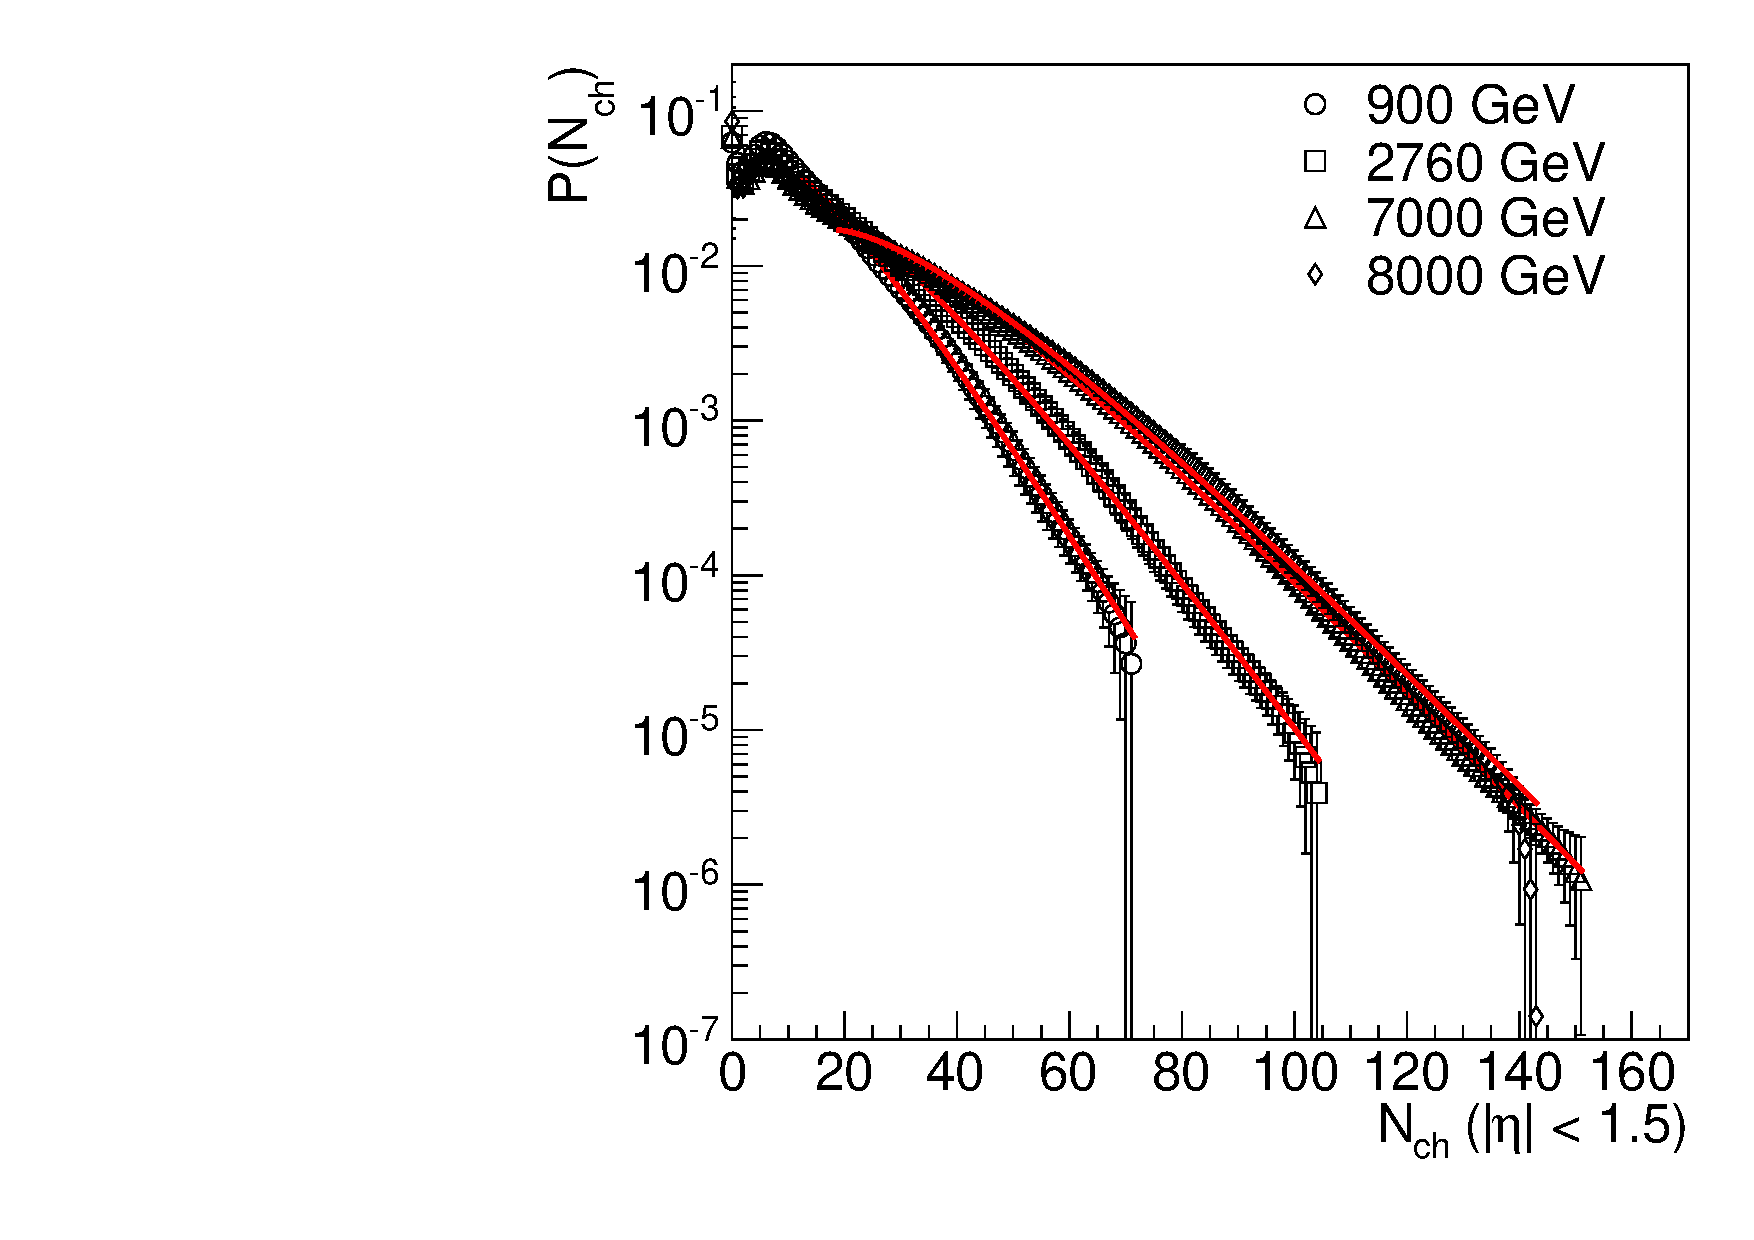
\includegraphics[width=0.49\linewidth]{\main/smallsystems/img/mult_data_1.pdf}
\hfill
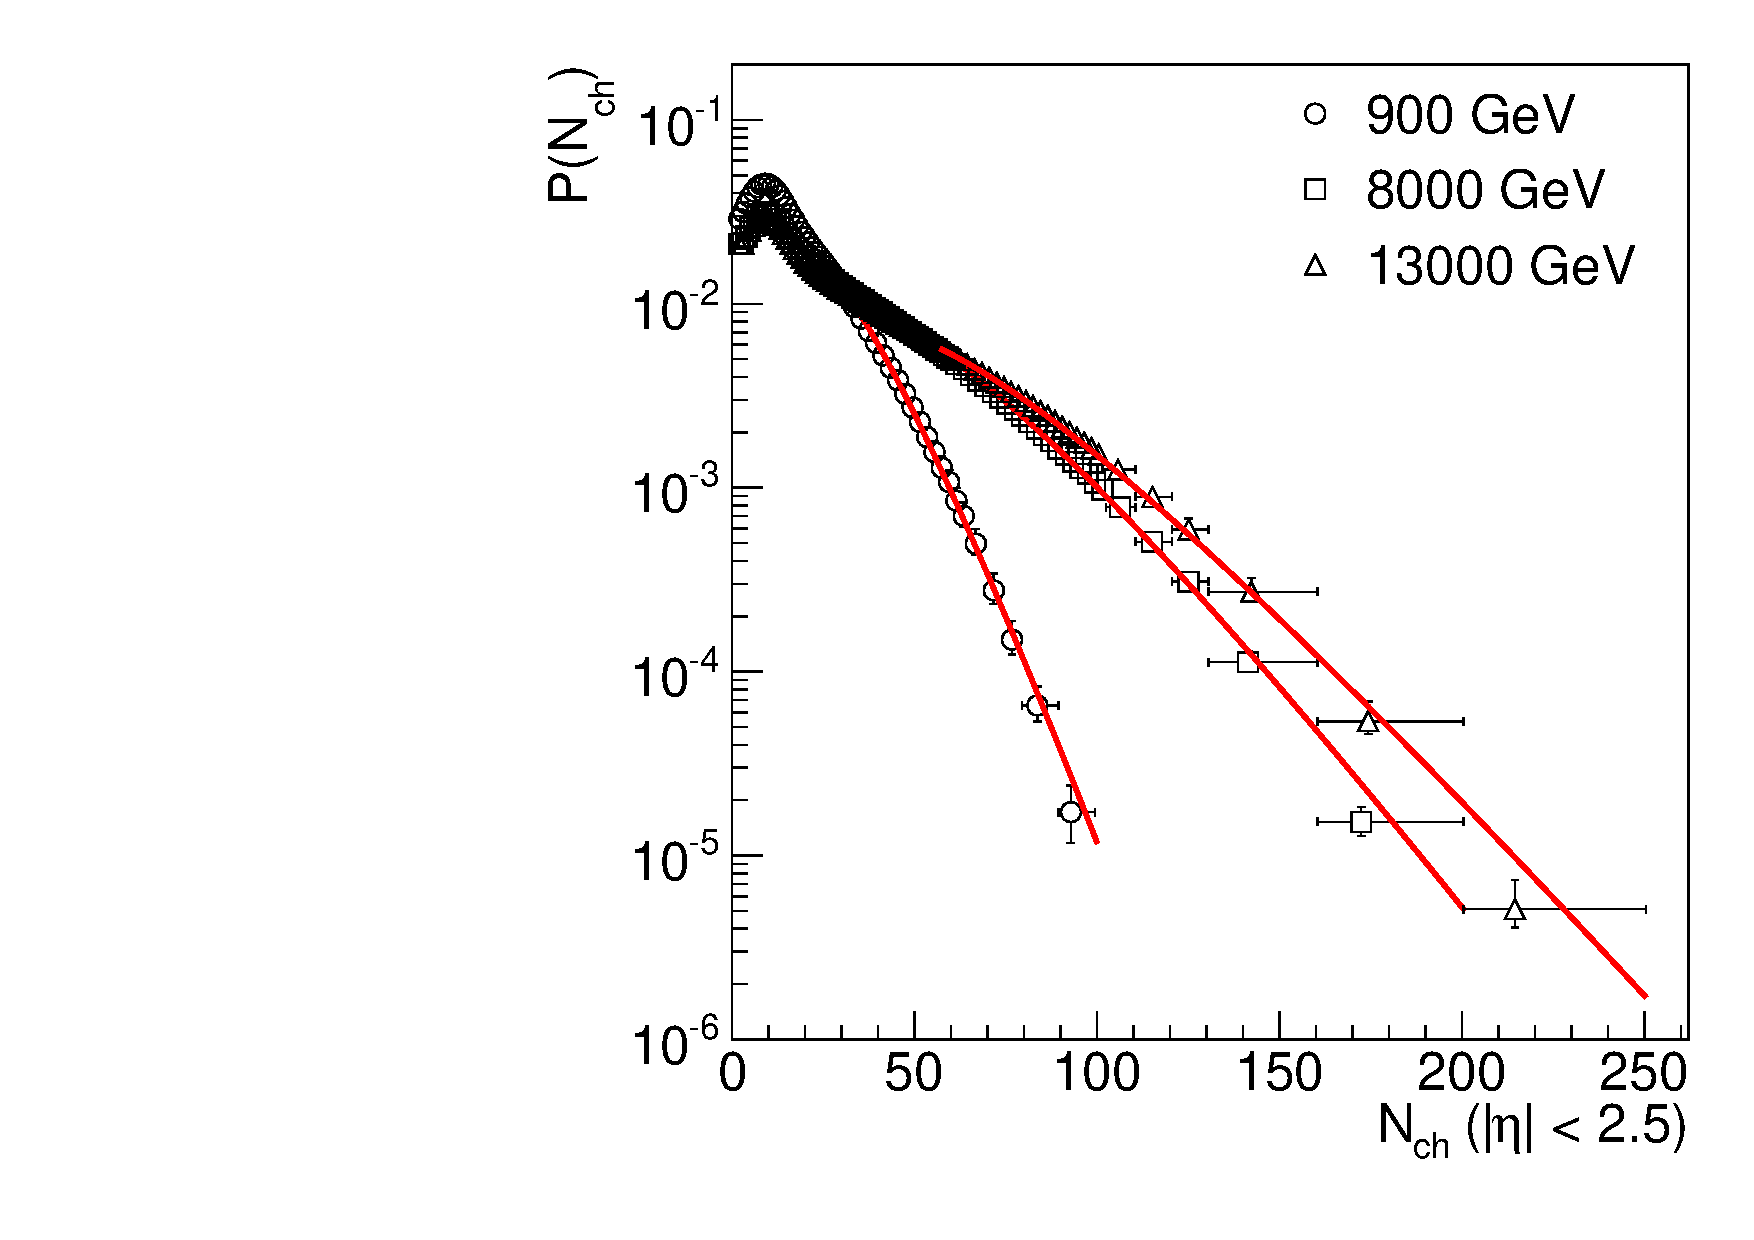
\includegraphics[width=0.49\linewidth]{\main/smallsystems/img/mult_data_11.pdf}
\caption{Multiplicity distributions measured by ALICE (left panel) and ATLAS (right panel) overlaid by the fit with a negative binomial distribution.}
\label{fig:smallsystems_mult_data}
\end{figure}

\begin{figure}[ht]
\centering
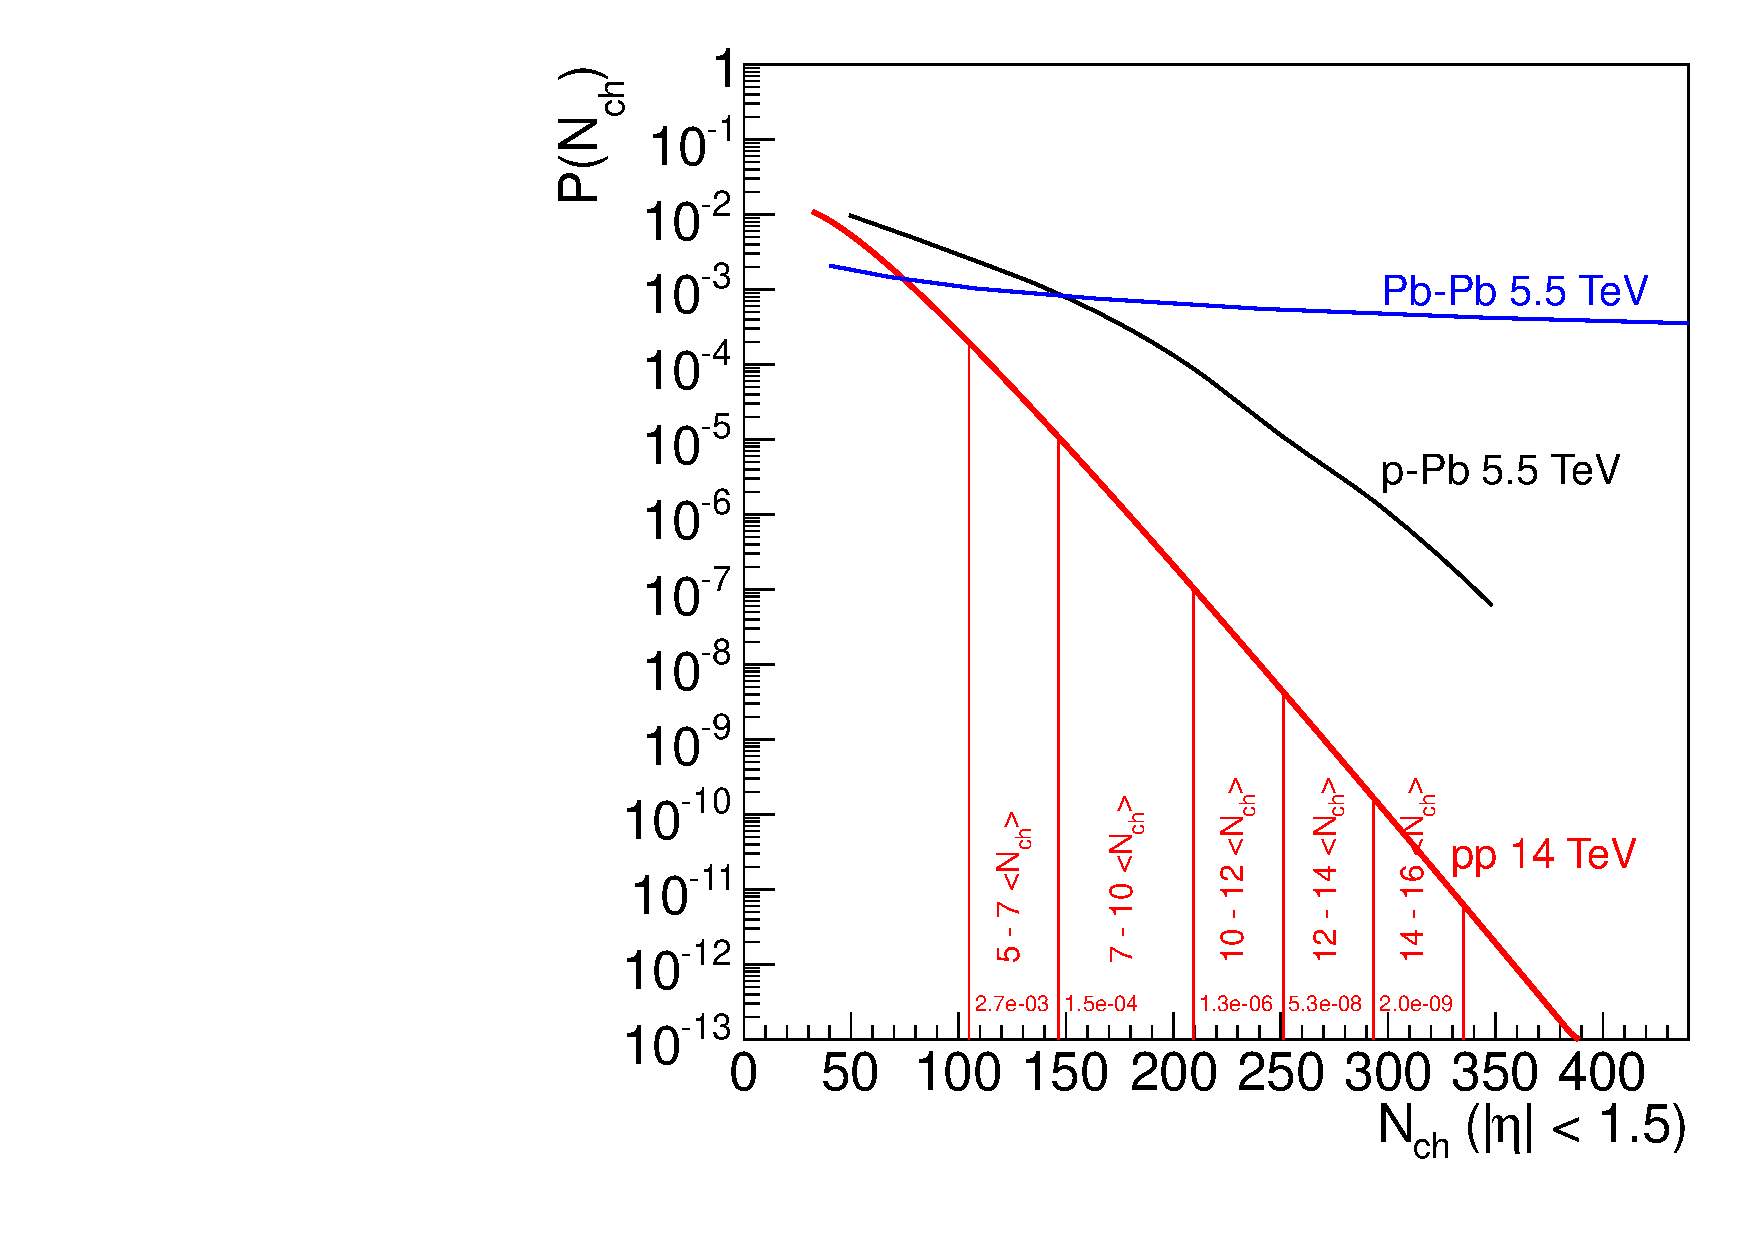
\includegraphics[width=0.32\linewidth]{\main/smallsystems/img/mult_extrapolation_1.pdf}
\includegraphics[width=0.32\linewidth,draft]{\main/smallsystems/img/mult_extrapolation_11.pdf}
\includegraphics[width=0.32\linewidth,draft]{\main/smallsystems/img/mult_extrapolation_11.pdf}
\caption{Extrapolated multiplicity distributions within $|\eta| < 1.5$ (left panel) and $|\eta| < 2.5$ (center panel) and scaled to the average multiplicity (right panel). The region of 14--16 \nch\ is indicated.}
\label{fig:smallsystems_mult_extrapolation}
\end{figure}

The resulting multiplicity distribution for 14~TeV is shown in Fig.~\ref{fig:smallsystems_mult_extrapolation} for the ALICE and ATLAS case. \todo{comment on comparison, and on general uncertainties of tail}. \todo{discuss comparison to pPb and PbPb}

\begin{table}
\centering
\begin{tabular}{c|c|c|c|c}
Range & $\dNdeta$ & Fraction & Events per pb$^{-1}$ & Events in 200~pb$^{-1}$ \\
\hline
5--7 \nch     & 35--49   & 2.4e-03       & 1.9e+08       & 3.7e+10 \\
7--10 \nch    & 49--70   & 1.3e-04       & 1.0e+07       & 2.0e+09 \\
10--12 \nch   & 70--84   & 1.1e-06       & 9.0e+04       & 1.8e+07 \\
12--14 \nch   & 84--98   & 4.7e-08       & 3.7e+03       & 7.3e+05 \\
14--16 \nch   & 98--112  & 1.8e-09       & 1.4e+02       & 2.8e+04 \\
\hline
\end{tabular}
\caption{Number of events in selected multiplicity bins at 14 TeV.}
\end{table}

\begin{table}
\centering
\begin{tabular}{l|c|c|c}
Range & $\dNdeta$ & Events per pb$^{-1}$ & Events in 200~pb$^{-1}$ \\
\hline
0--5\% p--Pb   & 41--56        & 4.9e+07       & 9.8e+09 \\
5--10\% p--Pb  & 34--41        & 1.9e+08       & 3.8e+10 \\
10--20\% p--Pb & 27--34        & 6.6e+08       & 1.3e+11 \\
20--40\% p--Pb & 20--27        & 2.7e+09       & 5.4e+11 \\
\hline
60--65\% Pb--Pb    & 98--137       & 1.5e+02       & 3.0e+04 \\
65--70\% Pb--Pb    & 68--98        & 1.6e+05       & 3.1e+07 \\ 
70--75\% Pb--Pb    & 45--68        & 2.1e+07       & 4.2e+09 \\
75--80\% Pb--Pb    & 29--45        & 5.9e+08       & 1.2e+11 \\
80--85\% Pb--Pb    & 18--29        & 4.6e+09       & 9.1e+11 \\
\hline
\end{tabular}
\caption{Number of events in pp collisions sliced in equivalent multiplicity bins in p--Pb and Pb--Pb collisions at 14 TeV.}
\end{table}


\todo{where to add which sigma(pp) used}

\subsubsection{Particle Correlations}

The measurements of two-particle correlations and higher-order cumulants have produced the initial observations of collectivity in small systems. In pp collisions, two distinct regions are of interest at HL-LHC: the high-multiplicity tail and the low-multiplicity regions. 

In pPb collisions, ...

\begin{figure}[ht]
\centering
\includegraphics[draft]{\main/smallsystems/img/corr_cumulants.pdf}
%\includegraphics[draft]{img/corr_cumulants.pdf}

\caption{Higher-order cumulants with and without applying subevents for pp (left) and pPb (right) as a function of Nch. ATLAS.}
\label{fig:smallsystems_corr_cumulants}
\end{figure}

\begin{figure}[ht]
\centering
\includegraphics[draft]{\main/smallsystems/img/corr_symmetriccumulants.pdf}
%\includegraphics[draft]{img/corr_symmetriccumulants.pdf}
\caption{Symmetric cumulants extracted with and without applying subevents for pp (left) and pPb (right) as a function of Nch. CMS.}
\label{fig:smallsystems_corr_symmetriccumulants}
\end{figure}

\begin{figure}[ht]
\centering
\includegraphics[draft]{\main/smallsystems/img/corr_cumulants_pid.pdf}
%\includegraphics[draft]{img/corr_cumulants_pid.pdf}

\caption{Particle identified $v_n$ (TODO only v2?) coefficients for pi, K, p (pp, ALICE), D mesons (pp, CMS), J/Psi (pp, pPb, ALICE, CMS) as a function of pT. Note that the multiplicity ranges are different for the different estimates. TODO: Plot may be messy and may need splitting in several panels.}
\label{fig:smallsystems_corr_cumulants_pid}
\end{figure}

\begin{figure}[ht]
\centering
\includegraphics[draft]{\main/smallsystems/img/corr_pvn.pdf}
%\includegraphics[draft]{\main/smallsystems/img/corr_pvn.pdf}

\caption{P(vn) estimate (ATLAS/ALICE).}
\label{fig:smallsystems_corr_pvn}
\end{figure}

\todo{p(vn)}

\subsubsection{Strangeness Enhancement}

\begin{figure}[ht]
\centering
\includegraphics[height=9cm]{\main/smallsystems/img/strangeness_omegapi.pdf}
%\includegraphics[height=9cm]{img/strangeness_omegapi.pdf}

\caption{$\Omega/\pi$ ratio as a function of $\nch$ in pp collisions. Black symbols denote existing data \cite{ALICE:2017jyt} and blue symbols extrapolation. TODO add syst unc scaled by factor 2}
\label{fig:smallsystems_strangeness_omega_pi}
\end{figure}

\subsubsection{Energy Loss}

Narrative: 
- Existing pA eloss measurements (ALICE, ATLAS, CMS) show limit of maximal few percent quenching. In conclusion, RpA is not a good observable
- Produce estimates for a) h-jet (a la ALICE), b) gamma-jet or Z-jet (ATLAS/CMS), c) jet substructure
- Produce these for pA and pp
- For pp, see if high mu sample can be also used for something. In fact it should be made clear where it can be used and where not, as this chapter will be one of the places where a low mu pp program is motivated.

\begin{figure}[ht]
\centering
\includegraphics[draft]{\main/smallsystems/img/energyloss_hjet.pdf}
%\includegraphics[draft]{img/energyloss_hjet.pdf}
\caption{Modification of jet recoil yields extracted from hadron-jet correlations for pp collisions (left) and p-Pb collisions (right). Delta-recoil ratio vs. pT.}
\label{fig:smallsystems_energyloss_hjet}
\end{figure}

\begin{figure}[ht]
\centering
\includegraphics[draft]{\main/smallsystems/img/energyloss_Zjet.pdf}
%\includegraphics[draft]{img/energyloss_Zjet.pdf}

\caption{Z-jet correlations in pp (left panel) and p-Pb collisions (right panel). 1/N dN/dxZj vs xZj.}
\label{fig:smallsystems_energyloss_Zjet}
\end{figure}

\subsubsection{Thermal Radiation}

\begin{figure}[ht]
\centering
\includegraphics[draft]{\main/smallsystems/img/thermal_radiation.pdf}
\caption{Thermal dileptons. Left panel: dN/Mee vs. Mee Example. Right panel: sensitivity as a function of Lint (pp, pPb) [expected signal is too uncertain].}
\label{fig:smallsystems_thermal_radition}
\end{figure}

\subsection{Data-taking strategy}

% High multiplicity triggering, pile up, MB sample
% pp
%   ALICE: additional several month pp program
%   ATLAS/CMS: special runs (mu~1) or special conditions at end of fill
%   LHCb: either in nominal (mu~5) or special running
%   HM sample: 200 pb-1 pp (per experiment)
%   How much MB for low-multiplicity questions?
% p-Pb scheduled run
%   1000-2000 nb-1

\subsection{Summary}

\bibliographystyle{report}   % Remember we use title in the biblio

\bibliography{section}
%% don't remove the folling lines, and edit the defintion of \main if needed
\documentclass[../report.tex]{subfiles}
\providecommand{\main}{..}
\IfEq{\jobname}{\currfilebase}{\AtEndDocument{\biblio}}{}
\IfEq{\jobname}{\currfilebase}{%file for shortcuts

\newcommand{\nch}{\ensuremath{N_{\mathrm {ch}}\xspace}}
\newcommand{\Ncoll}{\ensuremath{N_{\mathrm {coll}}}}
\newcommand{\Npart}{\ensuremath{N_{\mathrm {part}}}}
\newcommand{\dNdeta}{\mathrm{d}N_\mathrm{ch}/\mathrm{d}\eta}
\newcommand{\snn}         {\ensuremath{\sqrt{s_{\mathrm {NN}}}}}
\newcommand{\kT}          {\ensuremath{k_{\mathrm {T}}}}

\newcommand{\pp}          {pp}
\newcommand{\pPb}         {pPb}
\newcommand{\pA}          {pA}
\newcommand{\PbPb}        {PbPb}
\newcommand{\AuAu}        {AuAu}
\newcommand{\CuCu}        {CuCu}
\newcommand{\pAu}         {pAu}
\newcommand{\dAu}         {dAu}
\newcommand{\lsim}        {\,{\buildrel < \over {_\sim}}\,}
\newcommand{\gsim}        {\,{\buildrel > \over {_\sim}}\,}
\newcommand{\co}[1]       {\relax}
\newcommand{\nl}          {\newline}
\newcommand{\el}          {\\\hline\\[-0.4cm]}}{}
% until here


\begin{document}
\section{High energy QCD with proton-nucleus collisions and ultra-peripheral collisions}
%{ \small
\noindent {\bf Coordinator:} M. Winn (LAL, now DPhN, CEA/IRFU) %$^8$, now$^7$ 

\noindent {\bf Contributors:}
 A.~Angerami (LBNL Berkeley), %$^{18}$, 
 F.~Arleo (LLR/{\'E}cole Polytechnique), %$^5$, 
 N{.~Armesto (Universidade de Santiago de Compostela), %$^{17}$, 
 R.~Bin$^{21}$ (MIT), %, 
 {\'E}.~Chapon (CERN), %$^{23}$, 
 Z.~Citron (Ben Gurion University of Negev), %$^{13}$,
 J.~G.~Contreras~Nuno (Czech Technical University in Prague),  %$^1$, 
 M.~Dumancic (Weizmann Institute),
 D.~d'Enterria (CERN), %$^{23}$,
 G.~Giacalone (IPT CNRS/CEA), %$^6$, 
 V.~Guzey (Helsinki University, University of Jyvaskyla, Kurchatov institute, Gatchina),  %$^{2,3,16}$,  
 I.~Helenius (Universit\"{a}t T\"{u}bingen), % $^{12}$,
P.~Janus (AGH University of Science and Technology),
M.~Klasen (Universit\"{a}t M\"{u}nster), %$^{11}$, 
S.~Klein (LBNL Berkeley), %$^{18}$,
J.~Kremer (AGH University of Science and Technology),
 E.~Kryshen (Kurchatov institute, Gatchina), %$^{16}$, 
 A.~Kusina (Polish Academy of Sciences, Cracow), %$^{15}$,
 Y.-J.~Lee (MIT), %$^{21}$,  
 M.~van~Leeuwen (Utrecht University/Nikhef), %$^{14}$,  
 C.~Marquet (CPT/{\'E}cole Polytechnique), %$^{4}$, 
 C.~Mayer  (Polish Academy of Sciences, Cracow), %$^{15}$, 
 M.~Murray (University of Kansas),%$^{19}$,
 F.~Olness (SMU Dallas), %$^{22}$, 
 P.~Paakkinen (University of Jyvaskyla),%$^{3}$,  
 H.~Paukkunen (Helsinki University, University of Jyvaskyla), % $^{2,3}$,  
 I.~Schienbein (LPSC/Universit{\'e} Grenoble), %$^{9}$, 
 D.~Stocco (Subatech Nantes), %$^{10}$,  
 M.~Strikman (Pennsylvania State University), %$^{21}$,
 D.~Tapia~Takaki (University of Kansas). %$^{19}$.
}

% \bigskip
% \\
%{\footnotesize \it  
%${ ^{1}}$ Faculty of Nuclear Sciences and Physical Engineering, Czech Technical University in Prague, Prague, Czech Republic\\
%${^2}$ Helsinki Institute of Physics, University of Helsinki, Helsinki, Finland\\
%${^3}$ University of Jyvaskyla, Department of Physics,   Jyvaskyla, Finland\\
%${^4}$ Centre de Physique Th{\'e}orique, {\'E}cole Polytechnique, CNRS, Universit{\'e} Paris-Saclay, Palaiseau,  France\\
%${^5}$ Laboratoire Leprince-Ringuet, {\'E}cole Polytechnique, CNRS, Universit{\'e} Paris-Saclay, Palaiseau,  France\\
%${^6}$ Institut de physique th{\'e}orique, Universit{\'e} Paris-Saclay, CNRS, CEA, Gif-sur-Yvette, France \\
%${^7}$ Universit{\'e} Paris-Saclay Centre d'{\'E}tudes de Saclay (CEA), IRFU, D{\'e}partment de Physique Nucl{\'e}aire, Saclay, France \\
%${^8}$ Laboratoire de l'acc{\'e}l{\'e}rateur lin{\'e}aire, Universit{\'e} Paris-Sud, CNRS/IN2P3, Universit{\'e} Paris-Saclay, Orsay, France\\
%${^9}$ Laboratoire de Physique Subatomique et de Cosmologie, Universit{\'e} Grenoble Alpes, CNRS/IN2P3, Grenoble, France\\
%${^{10}}$ SUBATECH, IMT Atlantique, Universit{\'e} de Nantes, CNRS-IN2P3, Nantes, France\\
%${^{11}}$ Institut  f{\"u}r  Theoretische  Physik,  Westf{\"a}lische  Wilhelms-Universit{\"a}t  M{\"u}nster, M{\"u}nster,  Germany\\
%${^{12}}$ Institute f{\"u}r  Theoretische  Physik, Universit{\"a}t T{\"u}bingen, T{\"u}bingen, Germany\\
%${^{13}}$ Department of Particle Physics, Weizmann Institute of Science, Rehovot, Israel\\
%${^{14}}$ Institute for Subatomic Physics, Utrecht University/Nikhef, Utrecht, Netherlands\\
%${^{15}}$ The Henryk Niewodnicza{\'n}ski Institute of Nuclear Physics, Polish Academy of Sciences, Cracow, Poland\\
%${^{16}}$ National Research Center "Kurchatov Institute",
%Petersburg Nuclear Physics Institute (PNPI), Gatchina, Russia\\
%${^{17}}$ Departamento de F{\'i}sica de Part{\'i}culas and IGFAE,
%Universidade de Santiago de Compostela, Santiago de Compostela, Galicia-Spain\\
%${^{18}}$ Lawrence Berkeley National Laboratory, Berkeley, CA, USA\\
%${^{19}}$ Lawrence Livermore National Laboratory, Livermore, CA, USA\\
%${^{19}}$ The University of Kansas, Lawrence, KS, USA\\
%${^{20}}$ Massachusetts Institute of Technology, Cambridge, MA, USA\\
%${^{21}}$ Pennsylvania State University, University Park, PA, USA\\
%${^{22}}$ Southern Methodist University, Department of Physics, Dallas, TX,  USA\\
%${^{23}}$ CERN, European Organization for Nuclear Research, Geneva, Switzerland
%}

%{\footnotesize Acknowledgments: 
%NA was supported by Ministerio de Ciencia e Innovaci\'on of Spain under projects FPA2014-58293-C2-1-P, FPA2017-83814-P and Unidad de Excelencia Mar\'{\i}a de Maetzu under project MDM-2016-0692, by Xunta de Galicia (Conseller\'{\i}a de Educaci\'on) within the Strategic Unit AGRUP2015/11, and by FEDER. 

%The work of SK was supported by the U.S. Department of Energy, Office of Science, Office of Nuclear Physics, under contract DE-AC02-05-CH11231.

%The research of MS was supported by the U.S. Department of Energy, Office of Science, Office of Nuclear Physics, under Award No. DE-FG02-93ER40771.

%The research of FO was supported by the U.S. Department of Energy under grant  DE-SC0010129.

%MW acknowledges support from the European Research Council~(ERC) through the project EXPLORINGMATTER, founded by the ERC through a ERC-Consolidator-Grant.
% }
 


%Acknowledgements to be added:

%Mark Strikman: The research of M.S. was supported by the U.S. Department of Energy, Office of Science, Office of Nuclear Physics, under Award No. DE-FG02-93ER40771.

%N\'estor Armesto (Universidade de Santiago de Compostela)
%NA was supported by Ministerio de Ciencia e Innovaci\'on of Spain under projects FPA2014-58293-C2-1-P, FPA2017-83814-P and Unidad de Excelencia Mar\'{\i}a de
%Maetzu under project MDM-2016-0692, by Xunta de Galicia (Conseller\'{\i}a de Educaci\'on) within the Strategic Unit AGRUP2015/11, and by FEDER. 


%\textcolor{red}{Instructions/Comments}
%\begin{itemize}
%\item variable naming and unit conventions to be taken from review: https://arxiv.org/abs/0706.3356
%\item please have a look at the .sty-files to check for symbols to be used
%\item subsubsection may be omitted partially in final document, only working titles, please modify title if needed for your part, keep this structure for the moment to allow to separate different contributions more easily
%\item luminosities to be used: PbPb: 13 nb$^{-1}$ @ 5.5 TeV ATLAS/CMS/ALICE, LHCb to be seen, about a factor 10 less,
%pPb: 2000~nb$^{-1}$ @ 8.8 TeV for ATLAS/CMS, LHCb: 250~nb$^{-1}$@8.8~TeV for both orientation, 250~nb$^{-1}$ for ALICE @ 8.8 TeV for both configurations
%\item please keep for the moment the 'headers' for the subparts
%\item we should make an effort to stay within 20 pages, even if it is not easy
%\item authorship: there will be one common as much as possible inclusive list for the full chapter at the beginning.
%\end{itemize}


%    Plot labelling: Plots should contain the word "projection" if based on fiddling with numbers. Plots based on MC/simulation should contain the word "simulation".

%    Authorship. The first page of your chapter will contain
%        Coordinators: you
%        Contributors: alphabetical list of contributors to your chapter. Please start compiling this list and update Overleaf. The general guideline to include people who have contributed to either text, plots or substantially to important discussions. If you have doubt, please contact the conveners.
%        Please add them in the following format:
%        \textbf{Coordinators}: Donald Duck (CERN) and Daisy Duck (South Pole University)
%        \linebreak
%        \textbf{Contributors}: Jane (Brookhaven National Lab), John (CERN), Fred (LBNL)
%        Please compile this list until Oct 5, so that we can merge the author list for the front page of the report. Here the names will appear split in three groups: editors, coordinators, contributors

 %   Acknowledgements. Please add any needed acknowledgements (funding agencies etc.) to the file acknowledgements.tex in the base directory in Overleaf. Please follow the instructions in the file.

  %  Please use commands for symbols. The following symbols must be used, and should not be defined differently, or put as LaTeX "by hand". So e.g. always use \pT and not $p_{\rm T}$ even if it looks to produce the same at the moment. The list of most important symbols:
 %   \pT
 %   \kT, \nch, \meannch, \meanpT, \dNdeta, \dNdy
 %   \Lint, \sNN
 %   \pp, \pPb, \PbPb, etc.
 %   \UGeV, \UGeVc, \UGeVcc
%    [These commands are defined in cernall.sty, cernunits.sty and commands.tex.]
%    Please use the unit package for value unit combinations. E.g. \unit[1]{fm} instead of "1 fm" or "1~fm". I have seen that the acc. chapter has its own command. Probably you can just redefine that command to use \unit.

%%% 
%\setcounter{tocdepth}{4} 
%\tableofcontents

\subsection{Introduction}
\label{sec:smallxIntro}
%Editor: Nestor Armesto \\

Proton-nucleus~\cite{Salgado:2011wc} and ultraperipheral~\cite{Baltz:2007kq} collisions offer the opportunity to study the behaviour of QCD at high energies and large partonic densities~\cite{Kovchegov:2012mbw}. 
As the theory of the strong interaction, QCD is analytically well understood only in a perturbative regime of small coupling constant and where QCD radiation can be treated linearly, i.e. hadrons and nuclei are considered as dilute partonic objects. 
But non-linear effects are unavoidable in QCD, and they should eventually dominate at large densities to be achieved at high energies and for large nuclei. 
It was proposed long ago~\cite{Gribov:1984tu,Mueller:1985wy} that at such large densities a resummation of powers of density times coupling constant is possible, resulting in a non-perturbative but weak coupling regime where parton densities saturate, and whose effective field theory incarnation is the Color Glass Condensate~(CGC)~\cite{Gelis:2010nm}.
Particle production in pA collisions in the forward rapidity region is dominated by small$-x$ partons in the nucleus. 
Therefore, saturation effects are expected to be largest there. Furthermore, UPCs as a source of large fluxes of quasi-real photons, provide the opportunity to study the partonic structure of protons (in pp and pA) and nuclei (in pA and AA).

On the other hand, the structure of nucleons and nuclei, and the mechanism of particle production at small~$x$, are key ingredients for our understanding of heavy-ion collisions and for the characterisation of the produced hot dense medium. 
For hard probes, the nuclear modification of standard collinear parton densities is one of the uncertainties in the extraction of medium characteristics. 
For soft and semihard observables, both the parton densities and the detailed transverse structure of nucleons and nuclei are crucial ingredients for their description, e.g. for the initial conditions for hydrodynamical evolution~\cite{Liu:2015nwa,Weller:2017tsr,Mantysaari:2017cni}.

In the collinear framework, parton densities inside nuclei (nPDFs)~\cite{Paukkunen:2017bbm,armestodis2018} are poorly constrained due to two facts. 
On the one hand, data come from a large variety of nuclei and the number of data points for any of them, particularly for Pb for which it is less than 50 coming from fixed target DIS and DY experiments and from pPb collisions at the LHC, is very small compared to proton analysis. 
This fact makes the fit for a single nucleus impossible and the modeling of the $A$-dependence of the parameters in the initial conditions mandatory. On the other hand, the region covered by existing data is very small for the requirements of present hadronic colliders, see Fig.~\ref{fig:smallx1}. 
In spite of the uncertainties (in the applicability of collinear factorisation, scale choices, etc.) for their extraction in hadronic collisions and UPCs, these are the only experimental systems where they can be constrained before electron-ion colliders become available. 
The most up to date analysis include between 1000 and 2000 data points for 14 nuclei and are performed at next-to-leading accuracy~\cite{deFlorian:2011fp,Kovarik:2015cma,Eskola:2016oht} (even there exists some preliminary attempt at next-to-next-to-leading~\cite{Khanpour:2016pph}).
Differences between them mainly arise from the different sets of data included in the analysis and from the different functional forms employed for the initial conditions to be fitted. 
All in all, all parton species are very weakly constrained at small~$x<10^{-2}$, gluons at large~$x>0.2$, and flavour decomposition is largely unknown - a natural fact for $u$ and $d$ due to the approximate isospin symmetry in nuclei. 
The impact of presently available LHC data, studied in~\cite{Eskola:2016oht}, is quite modest with some constrains on the gluon in the region $0.01<x<0.3$. 
On the other hand, theoretical predictions for nuclear shadowing of quark and gluon PDFs  based on $s$-channel unitarity and diffractive nucleon PDFs are available down to $x \sim 10^{-4} \div 10^{-5}$, see~\cite{Frankfurt:2011cs,Armesto:2003fi} and references therein. 

\begin{figure}[htb]
\centering
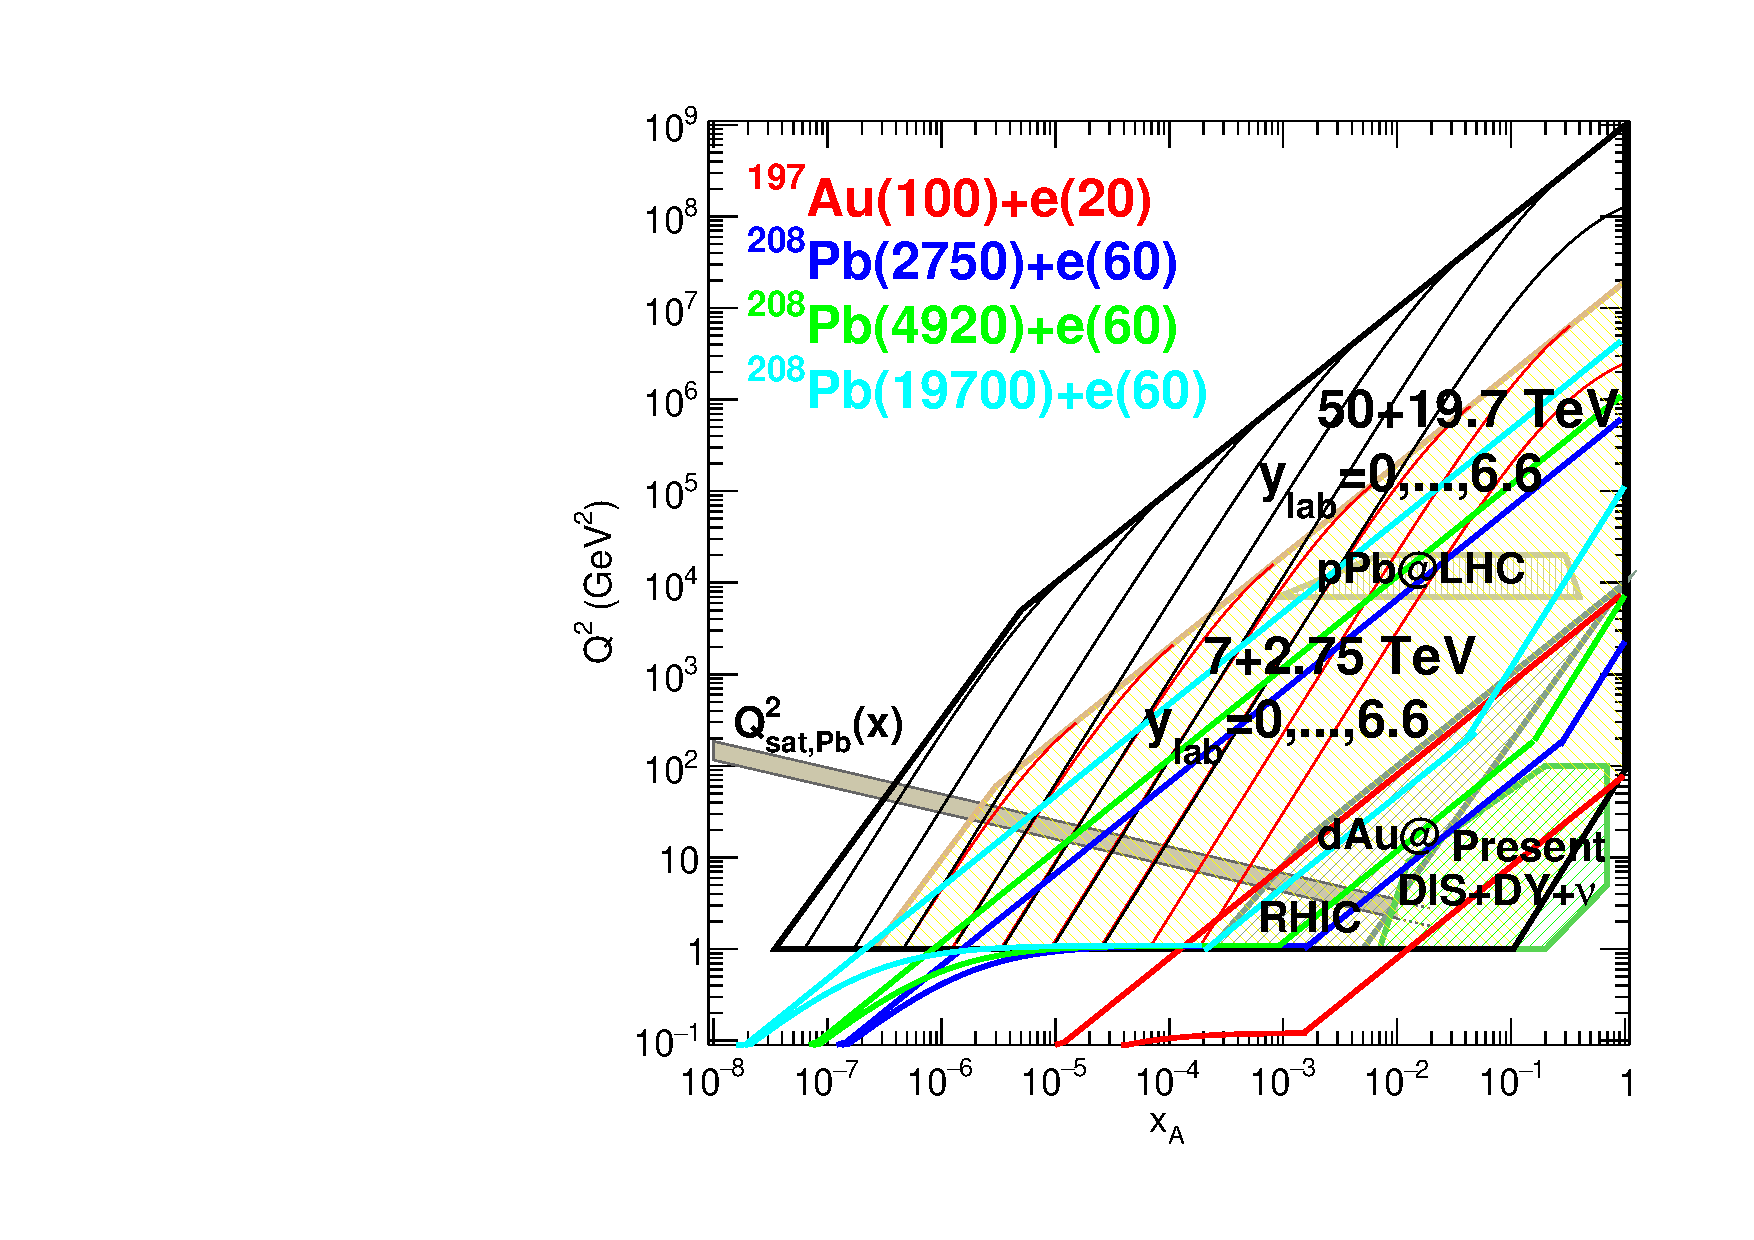
\includegraphics[width=0.45\textwidth]{\main/smallx/fig/FHC7_3.pdf} \hfill 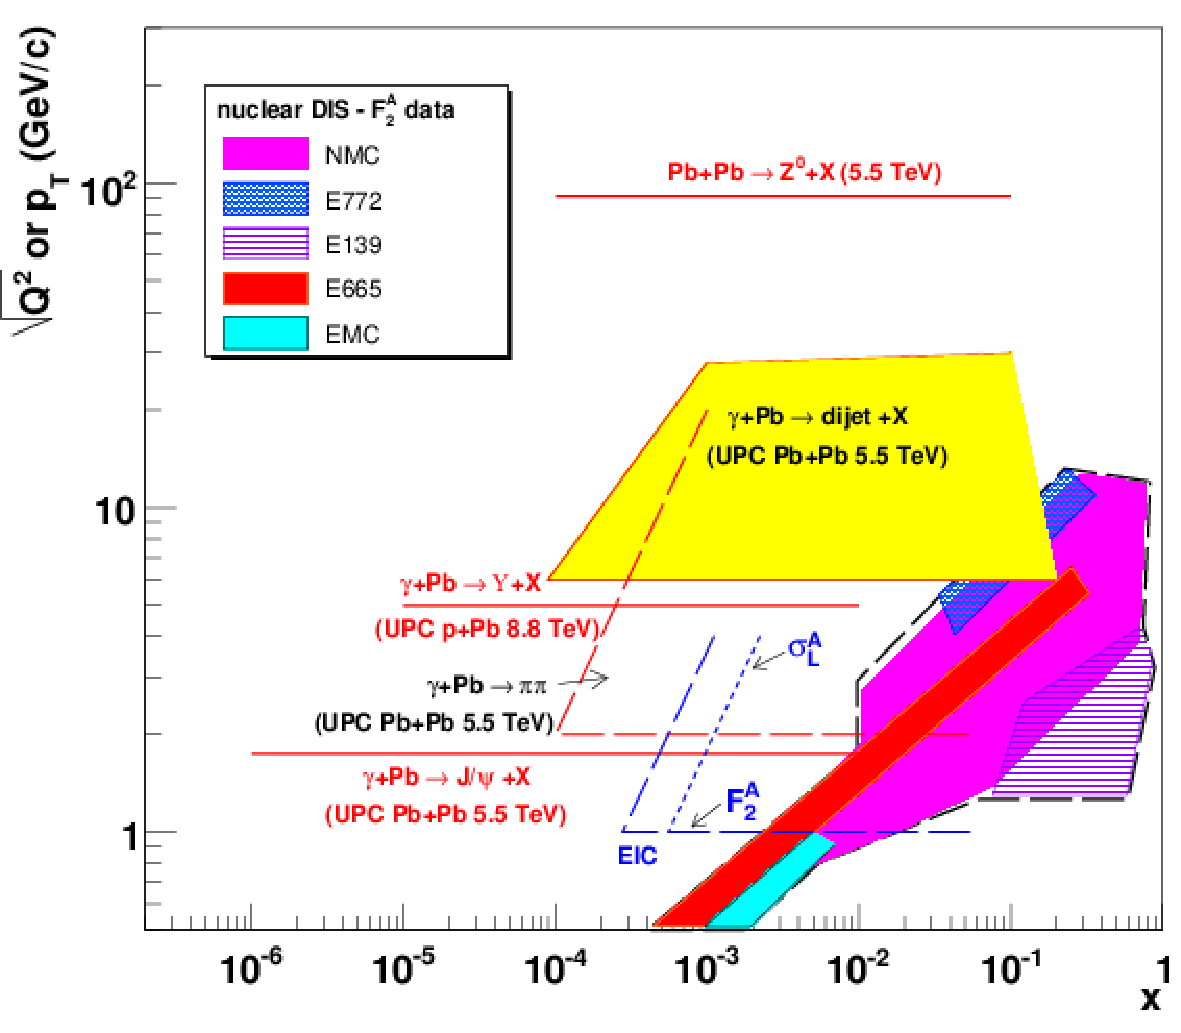
\includegraphics[width=0.45\textwidth]{\main/smallx/fig/upc_lhc_x_Q_map_5-eps-converted-to.pdf}
\caption{Left: $x$-$Q^2$ plane to be explored in proton-nucleus at the LHC and the FCC, and in  proposed electron-nucleus colliders, compared with the regions where the experimental data presently used in the EPPS16 analysis \cite{Eskola:2016oht} lie. Right: $x$-$Q^2$ plane to be explored in UPCs, taken from \cite{Baltz:2007kq}.}
\label{fig:smallx1}
\end{figure}

On the other hand, there have been recent claims~\cite{Ball:2017otu,Abdolmaleki:2018jln} that resummation of logarithms of $x$ may be required for a better description of DIS data from HERA at small $x$, and searches for long range azimuthal correlations are undergoing~\cite{zeusichep2018}. 
But no conclusive evidence of saturation (i.e. of non-linear dynamics) has been found in hadronic collisions. While the CGC provides a calculational framework for several observables in pp, pA and AA, see e.g. the reviews~\cite{Albacete:2013tpa,Lappi:2015jka}, like the ridge, back-to-back hadron correlations in the forward region, multiplicities and transverse momentum distributions,$\dots$,  the explanations are not unique or they involve non-perturbative modeling, or they are affected by large theoretical uncertainties and, for some of them, higher-order calculations are missing, or the data lie at the border of phase space where extracting clear conclusions is very delicate. 
Therefore, high-energy pA collisions and UPCs are the systems where data can offer clear evidences of non-linear effects at work.

In Fig.~\ref{fig:smallx1} we show the kinematic regions covered by proton-nucleus collisions at the LHC and the FCC~(left, \cite{Dainese:2016gch}) and UPCs at the LHC (right), compared with the regions where data currently used to constrain nPDFs lie.
A huge enlargement is evident. With respect to the presently existing data at the LHC, HL-LHC offers new improved detectors and larger statistics for some observables like dijets or photon-jet correlations, and the HE-LHC would enlarge the kinematic plane in a region intermediate between the LHC and the FCC. On the other hand, electron-nucleus collisions~\cite{AbelleiraFernandez:2012cc,Accardi:2012qut}, if they eventually happen in the 2030's, would be complementary, albeit in a more restricted kinematical region, by offering measurements in a cleaner experimental environment (no pileup, full kinematic reconstruction) and under better theoretical control as first-principle calculations are easier in DIS. 
The comparison between the kinematic regions covered by the LHC and Future Circular Collider~(FCC) in pA mode, and the Electron-Ion Collider~(EIC)~\cite{Accardi:2012qut} and the LHeC~\cite{AbelleiraFernandez:2012cc} (60 GeV electrons colliding with the HL-LHC, HE-LHC or FCC nuclear beams) is shown in Fig.~\ref{fig:smallx1} left.


\subsection{The physics of ultra-peripheral collisions}
%Editor: see sub-parts\\
%Indicative length: 6 pages\\
%Figures: to be discussed based on available experimental material, preference to full scale upgrade, should be balanced in terms of experiments as well as topics\\
%Tables: one large overview table for observables
\subsubsection{Experimental overview}
%Editors: Christoph Mayer(ALICE), Evgeny Krishen (ALICE), Daniel Tapia Takaki (CMS), Zvi Citron (ATLAS), Michael Winn (LHCb)
%Indicative length: 2 pages\\
%Content: observable overview table ordered by rate including back-of-envelope calculations for stat. error if nothing else available and explanations to instrumentation (one paragraph per experiment with suitable comparison with Run1/2), short mentioning of 'far beyond' observables in terms of luminosity in same collision system as default.

%intro MW
The four experiments at the LHC measured various processes in UPC during Run 1 and Run 2. In order to set the stage for the discussion of physics opportunities,  an overview of the detector capabilities in Run 3 and Run 4 is provided in the following. The expected statistics for show case observables is given in Tab.~\ref{tab:PbPbUPCrates,table:leadshine,table:protonshine} followed by the evaluation of the available precision for coherent heavy vector meson production and the theoretical assessment.

%ALICE paragraph draft CM
\begin{itemize}
\item In LHC runs 3 and 4, \textbf{ALICE}~\cite{Abelevetal:2014cna} will take data in
both in triggered and in continuous readout mode~\cite{Buncic:2015ari}. Using continuous
readout~\cite{Antoniolietal:2013} essentially the full delivered luminosity can be integrated
because there is no loss of statistics due to trigger
inefficiencies and dead-time. Therefore the acceptance for UPC events is significantly larger
than in LHC runs 1 and 2; it is determined by the tracking
efficiencies and the geometrical acceptances of the Inner Tracking
System (ITS)~\cite{Abelevetal:2014dna}, of the Time Projection Chamber (TPC)~\cite{ALICE:2014qrd}, and of the Muon Forward Tracker (MFT)~\cite{Uras:2012af}. The geometrical acceptances of these detectors correspond to the narrow central and forward acceptances in Tab.~\ref{tab:PbPbUPCrates},\ref{table:leadshine},\ref{table:protonshine}.
Final-state neutron emission in UPC events can be detected by the
zero-degree calorimeters (ZDC) which will also take data in continuous
readout mode, and vetoes can be imposed using the fast interaction
trigger detector~(FIT). %and the forward diffractive detector (FDD)
%ATLAS part by C. Z.
\item \textbf{ATLAS}
%CMS part by D.T.
\item \textbf{CMS}
%LHCb paragraph draft MW
\item \textbf{LHCb} is well suited for exclusive production studies in ultra-peripheral collisions. In particular, its optimisation for flavour physics within its acceptance 2$<\eta<$5 warrant an excellent resolution for typical momenta in quarkonium and heavy-flavour exclusive production as demonstrated in~Ref.\cite{LHCb-CONF-2018-003}. Its particle identification capabilities allow to measure final states with charged muons, pions, Kaons and protons. Exclusive diphoton analyses as pioneered in ATLAS~\cite{Aaboud:2017bwk} and CMS~\cite{CMS-PAS-FSQ-16-012} are also conceivable with lower \ET-thresholds discussed in Section~\ref{sec:upc}. The feasibility of inclusive $\gamma$-induced measurements will require further studies. In Tab.~\ref{tab:PbPbUPCrates},\ref{table:leadshine},\ref{table:protonshine} conceivable final states with suitable kinematic selections for analysis with LHCb are given.
\end{itemize}


The number of vector mesons expected in the upcoming runs can give us an estimate of the expected reach of HL-LHC.   To calculate this, we considered four toy-model experimental acceptances shown in Tab.~\ref{fig:UPCtoyacceptance}.  We did not estimate the effects of cuts on the $\pT$ of the final state daughter particles, because this depends fairly sensitively on the analysis and trigger conditions.   In general, for two-prong decays, as long as the minimum detectable $\pT$ is less than about 1/4 of the final state mass, $\pT$ cuts do not have a large effect.  We apply cuts to both the vector meson rapidity and the daughter particle pseudorapidities.  These cuts overlap greatly, and the results would not be very different without the cut on the vector meson rapidity. 

Table~\ref{tab:PbPbUPCrates} shows the expected cross-sections and rates for five representative vector meson decays, including the branching ratios.  The rates are calculated using STARlight~\cite{Klein:2016yzr}, which has been shown to do a good job of predicting the cross-sections for $\rho$~photoproduction on heavy targets~\cite{Adam:2015gsa,Abelev:2007nb}, and for all mesons on proton targets.  The $\rho$ is broad; here we consider the mass range from $2m_\pi$ up to $M_\rho + 5\Gamma_\rho$.  Direct $\pi^+\pi^-$~production is not included; this would add about 8\% to the rate.  
The $\rho'$ state is not well defined here, but is intended to represent $\pi^+\pi^-\pi^+\pi^-$ states with masses in the range from 4$m_\pi$ up to 2.5~\UGeVcc.  This could actually come from one or more states.  Since little is certain about the origin of this state or states, we anchor the calculation to the STAR measurement of the $\pi^+\pi^-\pi^+\pi^-$ final state~\cite{Abelev:2009aa} and use STARlight to extrapolate from gold to lead beams and upward in energy. 

The STARlight calculations do not yet include the effect of nuclear shadowing {\bf This needs to be done}, which will significantly reduce the rates for the heavy quarkonium.  Figure~\ref{fig:r} gives a pretty good estimate of the effect of shadowing.  

\begin{table}[h]
\begin{tabular}{|c|ccccc|}
\hline
Condition & Tot. & Central 1 & Central 2 & Forward 1 &  Forward 2   \\
                 &       & Narrow  & Wide    &      Narrow     &    Wide         \\
\hline
Rapidity & - & $|y|<0.9$ & $|y|<2.4$ & $2.5 < y < 4.0$ &   $2 < y < 5$ \\
$e/\pi/\mu$ pseudorapidity & - & $|\eta|<0.9$ & $|\eta|<2.4$  & $2.5 < \eta < 4.0$ & $2 < \eta <5 $ \\
\hline
\end{tabular}
\caption{Table of toy-model acceptance cuts for the different experiments.}
\label{fig:UPCtoyacceptance}
\end{table}

\begin{table}[h]
\begin{tabular}{|c|rrrrrr|}
\hline
\multicolumn{7}{|c|} {PbPb} \\
\hline
            &     $\sigma$              &  All          & Central 1   & Central 2   & Forward 1 & Forward 2 \\
Meson &                                 & Total        & Total          & Total          & Total         l &  Total  \\
\hline
$\rho\rightarrow\pi^+\pi^-$        & 5.2b & 68 B  & 5.5 B  & 21B & 4.9 B & 13 B \\
$\rho'\rightarrow\pi^+\pi^-\pi^+\pi^-$ & 730 mb & 9.5 B  & 210 M & 2.5 B & 190 M   & 1.2 B \\
$\phi\rightarrow K^+K^-$           & 0.22b & 2.9 B & 82 M & 490 M  & 15 M & 330 M  \\
$J/\psi\rightarrow\mu^+\mu^-$  & 2.5 mb & 32 M & 3.0 M & 15 M & 1.2 M &  3.3 M \\
$\psi'\rightarrow\mu^+\mu^-$    & 64$\mu$b & 830 K& 82 K & 410 K & 31 K &  79 K \\
$\Upsilon(1S)\rightarrow\mu^+\mu^-$ & 2.6 $\mu$b & 33 K & 4.0 K & 20K  & 880 &  2.0 K \\
\hline
\end{tabular}
\caption {Table of cross-sections and numbers of events in 13~nb$^{-1}$ integrated luminosity for the different mesons in PbPb collisions.   B, M and K denote $10^9$, $10^6$ and $10^3$ respectively. 
Both the rates and cross-sections account for the relevant branching ratio.}
\label{tab:PbPbUPCrates}
\end{table}

The rates for light mesons are enormous, enough to support billion-event samples of the $\rho$ and $\rho'$, and hundreds of millions of $\phi$, allowing the studies discussed below.  The rates for $J/\psi$, $\psi'$ and $\Upsilon (1S)$ should allow cross-section and tomographic measurements. 

In $\phi \rightarrow K^+K^-$, the kaons have a momentum of only 135 MeV/$c$ in the $\phi$ rest frame.  
The acceptance for this channel is quite low (even without a kaon $\pT$ cut), because the the kaon momentum is dominated by the $p_Z$ acquired from the $\phi$, so the kaons are produced with large pseudorapidity.   This channel is likely to be unobservable, except possibly at far forward rapidity, where the kaon momenta are significantly Lorentz boosted.  
Alternately, with enough data, it might be easier to search for $\phi \rightarrow \mu^+ \mu^-$ or $\phi \rightarrow e^+ e^-$, even though the branching ratios are small.
For a rough estimate, one could scale the $\phi\rightarrow K^+K^-$ rates down by Br ($\phi \rightarrow \mu^+ \mu^-$)/Br($\phi \rightarrow K^+K^-$)$\approx 5.9 \times 10^{-4}$ to conservatively estimate the rate to each dilepton channel; the acceptance for the dileptons should be higher than for the kaons. 

It should also be possible to explore photoproduction of double vector mesons by a single ion-ion pair (by exchange of two independent photons).  
The expected ratio of $\rho\rho$ photoproduction to single $\rho$ photoproduction is about $1:600$ while the predicted ratio of $\rho J/\psi$ to $\rho$ is about $1:160$ \cite{Klein:1999qj}.  
These events should display significant quantum correlations.  

For pA collisions, there are additional complications, in that the per-nucleon center of mass is boosted by 0.465 units of rapidity from the lab frame, and because there are two possible directions for the beams (protons from the $+z$ direction, or from the $-z$ direction); this makes a big difference for forward detectors.  There are also two possibilities for the photon emitter, 'lead-shine' or 'proton-shine.'  These have rather different kinematics, with the vector meson $\pT$ scale set by the size of the nuclear target, $\hbar/R_{\rm proton}$ or $\hbar/R_{\rm Pb}$ respectively.    So, we calculate the rates for these two possibilities in separate tables.

We assume that the total $pPb$ luminosity of 2000 nb$^{-1}$ is equally divided between the two possible proton beam directions.  For the asymmetric (around $y=0$) detectors, we consider these two runs separately, listing them as 'forward' (in the proton-going hemisphere) and 'backward' (in the lead-going hemisphere).  

We have not attempted to calculate the rates for the $\rho'$ because of uncertainty in the rates on the proton targets.  

Tables~\ref{table:leadshine} and~\ref{table:protonshine} show the cross-sections and rates for the leadshine and protonshine cases respectively. 

\begin{table}[h]
\begin{tabular}{|c|rrrrrrrr|}
\hline
\multicolumn{9}{|c|} {pPb - lead shine} \\
\hline
            &     $\sigma$              &  All & Ctl. 1 & Ctl. 2 & FW 1 & FW 2 & BW 1 & BW 2 \\
Meson & & Total & Total & Total &Total  & Toal  & Total & Total \\
\hline
$\rho\rightarrow\pi^+\pi^-$ & 35 mb& 70 B & 3.9 B& 15 B& 2.0 B & 5.5 B& 850 M& 2.0 B\\
%$\rho'\rightarrow\pi^+\pi^-\pi^+\pi^-$ $ & & & & & &  & & \\
$\phi\rightarrow K^+K^-$ & 870 $\mu$b & 1.7 B & 65 M & 290 M & 22 M &120 M  &9.7 M  & 52 M\\
$J/\psi\rightarrow\mu^+\mu^-$ & 6.2 $\mu$b  & 12 M & 1.0 M &5.2 M & 260 K & 800 K  & 180 K & 430 K\\
$\psi'\rightarrow\mu^+\mu^-$   &134 nb & 270 K & 22 K & 110 K & 6.0 K &  18 K & 3.2 K & 7.7 K \\
$\Upsilon(1S)\rightarrow\mu^+\mu^-$ & 5.74 nb & 11 K &  1.1 K & 5.4 K & 310 & 880  & 41 & 100 \\
\hline
\end{tabular}
\caption {Table of cross-sections and numbers of events for the different mesons in pPb collisions for 'lead-shine' (a photon from the lead scattering from the proton).  The rates are for the 2000 nb$^{-1}$ integrated luminosity noted above, split evenly between the two possible proton directions.  For the central regions, the net luminosity is 2000 nb$^{-1}$  since both directions contribute, but for the forward (FW) and backward (BW) directions, the net luminosity is only 2000 nb$^{-1}$ each. B, M and K denote $10^9$, $10^6$ and $10^3$ respectively. 
Both the rates and cross-sections account for the relevant branching ratio.}
\label{table:leadshine}
\end{table}

\begin{table}[h]
\begin{tabular}{|c|rrrrrrrr|}
\hline
\multicolumn{9}{|c|} {pPb - proton shine} \\
\hline
            &     $\sigma$              &  All & Ctl. 1 & Ctl. 2 & FW 1 & FW 2 & BW 1 & BW 2 \\
Meson & & Total & Total & Total & Total & Total  & Total & Total \\
\hline
$\rho\rightarrow\pi^+\pi^-$ & 531$\mu$b & 1.1 B& 83 M  &360 M & 20 M & 44 M & 56 M& 150 M \\
%$\rho'\rightarrow\pi^+\pi^-\pi^+\pi^-$ & & & & & &  & & \\
$\phi\rightarrow K^+K^-$ &  23 $\mu$b &46 M & 1.3 M & 8.0 M & 120 K & 1.7 M  & 210 K & 3.9 M \\
$J/\psi\rightarrow\mu^+\mu^-$ &  333 nb & 670 K  & 55 K & 290 K & 14K & 36 K  & 15 K & 41 K\\
$\psi'\rightarrow\mu^+\mu^-$   & 8.9 nb & 18 K & 1.5 K & 7.9 K & 380 & 990  & 380 &  1.0 K  \\
$\Upsilon(1S)\rightarrow\mu^+\mu^-$ & 0.43 nb &  860 & 93  & 460 & 14 & 34 & 14 &  30 \\
\hline
\end{tabular}
\caption {Table of cross-sections and rates for the different mesons in pPb collisions for 'proton-shine' (a photon from the proton scattering from the lead nucleus).  The rates are for the 2000 nb$^{-1}$ integrated luminosity noted above, split evenly between the two possible proton directions.  For the central regions, the net luminosity is 2000 nb$^{-1}$  since both directions contribute, but for the forward (FW) and backward (BW) directions, the net luminosity is only 2000 nb$^{-1}$ each. B, M and K denote $10^9$, $10^6$ and $10^3$ respectively. 
Both the rates and cross-sections account for the relevant branching ratio.}
\label{table:protonshine}
\end{table}




%transition piece by MW
In case of coherent heavy vector meson production in UPC, a detailed evaluation of the expected performance is undertaken for ALICE and CMS.

%E. K., C.M., D. T.
Vector meson cross section in Pb-Pb UPC can be expressed as a sum of two terms reflecting the fact that either of the colliding ions can serve as a photon source:
\begin{equation}
\sigma(y) = n(+y) \sigma_{\rm \gamma Pb}(+y) + n(-y) \sigma_{\rm \gamma Pb}(-y)
\end{equation}
The photoproduction cross sections $\sigma_{\rm \gamma Pb}(y)$ and $\sigma_{\rm \gamma Pb}(-y)$ are coupled and cannot be extracted unambiguously from the measured rapidity differential cross section. However, one can decouple them by measuring vector meson production in UPC with and without additional neutron activity in Zero Degree Calorimeters~\cite{Guzey:2013jaa}. Measurement of $\sigma_{\rm 0N0N}(y)$ (no neutrons on both sides) and $\sigma_{\rm 0NXN}(y)$ (at least one neutron on one of the sides) cross sections provides a system of two equations of two unknown photoproduction cross sections $\sigma_{\rm \gamma Pb}(\pm y)$:
\begin{eqnarray}
\sigma_{\rm 0N0N}(y) &=& n_{\rm 0N0N}(+y) \sigma_{\rm \gamma Pb}(+y) + n_{\rm 0N0N}(-y) \sigma_{\rm \gamma Pb}(-y), \\
\sigma_{\rm 0NXN}(y) &=& n_{\rm 0NXN}(+y) \sigma_{\rm \gamma Pb}(+y) + n_{\rm 0NXN}(-y) \sigma_{\rm \gamma Pb}(-y),
\end{eqnarray}
where $n_{\rm 0N0N}(\pm y)$ and $n_{\rm 0NXN}(\pm y)$ are corresponding photon fluxes, calculable with high accuracy.

Solutions of this system of equations can be used to extract gluon shadowing at different scales under the assumption that the coherent photoproduction cross section is proportional to the squared gluon density at the scale $Q = m_{V}/2$. In this case, one can construct the nuclear suppression factor expressed as root square of the ratio of photoproduction cross section measured in Pb-Pb UPC and photoproduction cross section in the Impulse Approximation calculated as a reference photoproduction cross section off proton scaled by the integral over squared Pb form factor~\cite{Guzey:2013xba}:
\begin{equation}
R_{\rm Pb} (x) = \left(\frac{\sigma_{\rm \gamma Pb}(x)}{\sigma_{\rm IA}(x)}\right)^{1/2}, \qquad {\rm where}\qquad x  = \frac{m_{V}}{\sqrt{s_{NN}}}\exp(-y).
\end{equation}
Resulting projections for the nuclear suppression factor are shown in Fig.~\ref{fig:r} at different scales corresponding to $J/\psi$, $\psi(2S)$ and $\Upsilon(1S)$ photoproduction measurements. Uncertainties on luminosity (4\%), reference cross section (5\%) and photon flux (5\%) result in $\sim8$\% systematic uncertainty on the ratio $\sigma_{\rm \gamma Pb}(x)/\sigma_{\rm IA}(x)$ and $\sim 4$\% uncertainty on the nuclear suppression factor $R_{\rm Pb} (x)$.

\begin{figure}
\centering
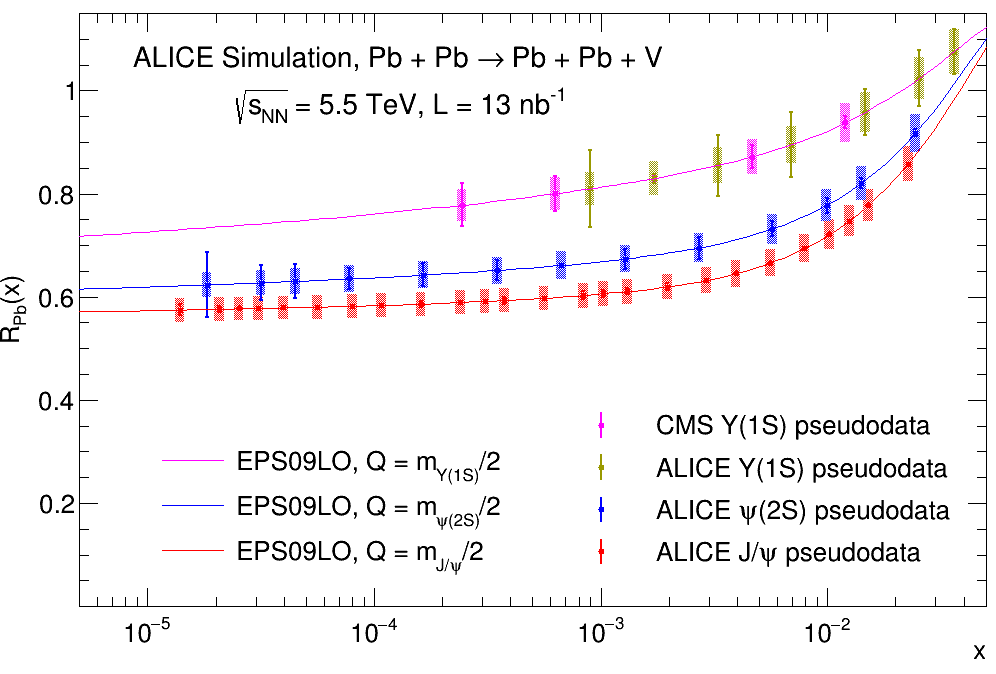
\includegraphics[width=0.6\textwidth]{\main/smallx/fig/suppression_factor.png}
\caption{Projections for gluon shadowing factor measured with heavy vector photoproduction in Pb-Pb UPC collisions at different scales.}
\label{fig:r}
\end{figure}

\subsubsection{Vector meson production}
%Editors: Mark Strikman and Vadim Guzey + Jesus Guillermo Contreras Nuno + Spencer Klein\\
%Indicative length: 1-2 pages

\subsubsubsection{Coherent vector meson production off nuclei}
%\subsection{}

Extensive data were produced in the previous LHC heavy ion runs on coherent photoproduction  of $\rho$ mesons~\cite{Adam:2015gsa}, 
$J/\psi$~\cite{Abbas:2013oua,Abelev:2012ba,Khachatryan:2016qhq} and to a lesser extent $\Psi'$~\cite{Adam:2015sia}: 
$\gamma+ A \to V +A$. Due to the presence of two photon sources, the $x$-range of these studies is largely  limited
to $x\ge m_V/\sqrt{s}$. For light mesons these measurements provide information on the pattern of interactions of extended pion-size mesons and such phenomena as shadowing and color fluctuations. For small dipoles like $J/\psi$ and $\Upsilon$, 
it provided information on the leading twist nuclear shadowing at moderate $Q^2$, which is difficult to obtain using other hard probes. A factor of $\sim 3$ reduction of the $J/\psi$ 
cross section compared to the $\gamma p$ case is consistent with the expectation of the leading twist 
approximation~\cite{Guzey:2013xba,Guzey:2013qza} and substantially stronger than that in the dipole 
model~\cite{Lappi:2013am} (in this case, the shape and normalization of the rapidity distribution rather 
strongly depends on the form of the dipole cross section and charmonium wave function).
In the case of $\rho$ meson production, shadowing is a factor of $\sim 2$ stronger~\cite{Frankfurt:2015cwa} than in the approach based on
the Glauber model and the vector meson dominance model.

The higher LHC luminosity and experimental upgrades will allow us to collect vastly improved samples of UPC events.   In particular, the planned ALICE continuous readout \cite{Krivda:2017sto}, will eliminate many of the trigger-based constraints that have limited UPC data collection, allowing for high-efficiency collection of very samples of photoproduced light mesons.   The increases in sample sizes should be considerably larger than one would expect from scaling the luminosity.  
\begin{itemize}
\item
Extend substantially the $x$ range for coherent $J/\psi$ photoproduction on nuclei
using information on the centrality of collisions using forward neutron production~\cite{Guzey:2013jaa}
 as well as using $pA$ scattering. In the later case, one would have to separate coherent $J/\psi$ production in $\gamma A$ and $\gamma p$  using a much more narrow $\pT$ distribution of $J/\psi $ produced in coherent $\gamma A$ scattering
 and very good $\pT$ resolution for the transverse momentum of the pair (LHCb).
\item
Measure with high enough  statistics coherent $\Upsilon $ production in $\gamma p$ and $\gamma A$
scattering to check the expectation of the 20\% reduction of the coherent cross section, which would allow one to probe gluon shadowing at a factor of $\sim 10 $ higher $Q^2$ than in $J/\psi$ production.
\item
Study coherent production of two pions with masses above 1~\UGeVcc to study an interplay of soft and hard dynamics as a function of $M_{\pi \pi}$ and $\pT(\pi)$.   
\item
Measure the production of heavier $2\pi$ \cite{Klein:2016dtn}, $4\pi$ and other resonances on ion targets, and search for the photoproduction of the observed exotic mesons.  
By using data from both proton targets (at HERA or the LHC) and ion targets, it is possible to separate the photon-meson coupling constant and the meson-nucleon interaction cross-sections.  
\item
Study the photoproduction of multiple vector mesons by a single ion pair \cite{Klein:1999qj}.   Double photoproduction introduces many quantum correlations, including the possibility of observing stimulated decays of vector mesons.  Also, since the two photons share the same linear polarization, is will be possible to study photoproduction with polarized photons.

\end{itemize}

\subsubsubsection{Nuclear Imaging with coherent photoproduction}

In coherent photoproduction, production amplitudes from each individual scattering site add, with a phase factor $\exp{i(\vec{x}\cdot\vec{k})}$, where $\vec{x}$ is the location within the nucleus, and $\vec{k}$ is the momentum transfer from the nucleus to the vector meson.  So, one can Fourier transform the coherent photoproduction cross-section, $d\sigma_{\rm coherent}/dt$ to find the location of the scattering sites within the nucleus.  This can provide information on the spatial dependence of nuclear shadowing, allowing us to compare shadowing in the center of nuclei vs. shadowing in the periphery through the transverse profile $F(b)$.   Assuming azimuthal symmetry \cite{Diehl,Toll:2012mb}
\begin{equation}
F(b) \propto \frac{1}{2\pi} \int_0^\infty  \pT d\pT J_0(b p_T) \sqrt{\frac{d\sigma_{\rm coherent}}{dt}}.
\end{equation}
One complication is that it is necessary to flip the sign of $\sqrt{d\sigma_{\rm coherent}/dt}$ when crossing each diffractive minimum in the sample.

This calculation is  data-hungry, and is subject to a number of theoretical uncertainties.  It is also necessary to separate the cross-section into its coherent and incoherent components.  Nevertheless, the STAR Collaboration applied it to $\rho^0$ photoproduction in UPCs \cite{Adamczyk:2017vfu}, finding a relatively boxy shape, inconsistent with a Woods-Saxon distribution, but seemingly consistent with expectations from nuclear shadowing.   A follow-on study explored the  $Q^2$~evolution of this transverse distribution by dividing the sample into three bins with different dipion mass \cite{Klein:2018grn}.  That study also considered some of the uncertainties inherent in the analysis, including the finite experimental reach in $\pT$ and the effects of the photon$\pT$, and the impact of the vector meson wave function. 

Studies at the LHC could avoid many of these issues, by triggering on exclusive vector mesons (STAR required that the vector mesons be accompanied by neutrons from mutual Coulomb excitation).  This would expand the $\pT$ range where a meaningful $d\sigma_{\rm coherent}/dt$ can be extracted, increasing the accuracy of the transform.  Also, because of the higher beam energies, the photon~$\pT$ is less important than it is at RHIC.    More importantly, HL-LHC could also extend this study to a wider variety of mesons, including the $\rho'$ (generically, $4\pi$ final states with a mass in the 1-2 \UGeVcc range) and the $J/psi$.  The latter is of particular interest because it is heavy enough to probe gluon shadowing, rather than just nuclear shadowing.  

\subsubsubsection{Incoherent vector meson production off nuclei}

Incoherent diffractive processes provide information on nuclear dynamics,  which is complementary to the 
information one can obtain from 
coherent scattering. In particular, incoherent $J/\psi$ photoproduction  probes quantum fluctuations of the target gluon density~\cite{Frankfurt:2008vi,Mantysaari:2016ykx,Mantysaari:2016jaz,Mantysaari:2017dwh,Cepila:2016uku,Cepila:2017nef}.
The corresponding cross section can be measured a much larger range of $W_{\gamma N}$ than in the coherence case since one can 
determine  (by detecting activity in the nucleus fragmentation region, for example, neutrons in a ZDC) which of two nuclei was a source of photons practically in each event.

One can distinguish two contributions to incoherent diffraction: 
quasielastic, when the nucleus involved in the strong interaction breaks down into nucleons and nuclear fragments, 
and inelastic, when hadrons are produced in the nucleus fragmentation  region.
% in the rapidity interval $\Delta y= y_{max} - y_{act}$. 
At small $t$ the second  mechanism gives a $\sim 20\% $ contribution to the incoherent cross section. However, since the $t$-dependence of the inelastic  mechanism is weaker, it dominates the nuclear incoherent cross section for $|t| \ge 0.5$ GeV$^2$. 

While it is generally understood and accepted that $J/\psi$ photoproduction with target dissociation is sensitive to fluctuations
of the gluon density of the target, practical realizations of this notion require modeling. Notably, 
proton size fluctuations at $t=0$~\cite{Frankfurt:2008vi} should be contrasted with proton shape fluctuations~\cite{Mantysaari:2016ykx,Mantysaari:2016jaz,Mantysaari:2017dwh}, which in turn
can be refined by including fluctuations of number of hot spots~\cite{Cepila:2016uku,Cepila:2017nef}; the latter two approaches 
are assumed to be valid in an entire range of $|t|$.
Hence, studies of incoherent diffraction
in $\gamma p$ scattering via $pA$ UPCs and $\gamma A$ scattering via $AA$ UPCs would allow one to map variations of the gluon fluctuations with energy ($x$) including a possible approach to the black disk regime, where the 
fluctuations are strongly suppressed~\cite{Cepila:2016uku}.

For very large $|t| \ge 1 - 2$ GeV$^2$ one enters the regime of pQCD, which corresponds to elastic scattering of small-size dipoles
off individual small-$x$ partons of the nuclear target~\cite{Frankfurt:2008et,Frankfurt:2008er}.

Note also that for the proton target, one can use the process  $\gamma + p \to VM (J/\psi) + gap + Y$  at   
$-t \ge \mbox{few GeV}^2$ to study the perturbative Pomeron. 
In the kinematics, where $\Delta y$ is fixed, 
$d\sigma /dy_{VM} \propto (y_{VM}- \Delta y)^{2\alpha_{Pomeron}-2}$. In BFKL one expects
$2\alpha_{Pomeron}-2\sim 0.4$ and, hence, a strong rapidity dependence of the corresponding cross section. A larger acceptance of the ATLAS and CMS detectors allows for a more effective study of these processes than at HERA.


By studying the $t$-dependence and activity in the nucleus 
fragmentation region it would be possible to separate the two mechanisms of incoherent nuclear scattering as a function of $t$.
For small $|t| \le 0.3 - 0.5$ GeV$^2$, one can calculate nuclear shadowing for both mechanisms within the leading 
twist shadowing framework~\cite{Guzey:2013jaa}. The shadowing turns out to be large and sensitive to the details of the leading twist shadowing dynamics.  At large $|t|$, one can study the $A$ dependence of the discussed reaction for different rapidity gap  
intervals to track propagation of a small dipole through the nuclear medium.
 By changing $\Delta y$ it would be possible to vary  strongly the relative role of the initial and final state interaction.


\subsubsection{Photoproduction of heavy quarks}
%Author: Spencer Klein\\
%Indicative length: 0.5-1 page
\label{sec:upchqdijets}

Photoproduction of open charm and bottom is a direct probe of the gluon content of the target nucleus \cite{Klein:2002wm,Goncalves:2017zdx}.  The lowest order process, $\gamma + gluon\rightarrow c \overline c$ (or $b \overline b$) dominates over higher order, resolved processes, in which the photon radiates before it interacts with the target gluon \cite{Klein:2002wm}.  This process has some similarities with photoproduction of dijets, discussed below.  

However, open charm offers some advantages.  Vertex detectors can detect separated vertices from charm production if the charm is moderately relativistic \cite{Bala:2012vg}, so it should be possible to study pairs with an invariant mass of $M_{c\overline c} \approx 4m_c$.  This will enable us to study gluon distributions down to Bjorken$-x$ values of around: $x \approx M_{Q\overline Q}/4\gamma m_p \exp(y)$.  The corresponding scale is $Q^2 \approx M_{Q\overline Q}$.  This is considerably lower Bjorken$-x$ than for dijets, where the minimum mass is 10-20~\UGeVcc.  By comparing results from proton targets (in $pA$ collisions) and heavy-ion targets (in $AA$ collisions), it is possible to make a fairly clean measurement of nuclear shadowing.  

The experimental signature is fairly clear: a pair of separated vertices (or a separated vertex and a lepton with a large impact parameter) in an event with one large rapidity gap. The ion near the rapidity gap should also remain intact. 

The main disadvantage is the need to reconstruct both the charmed hadron and the anti-charmed hadron.  It may also be possible to make useful measurements from one fully reconstructed meson, and one semileptonic decay, but this needs to be studied.  However, the charm production rates are high enough so that the low efficiency is not too big a problem.

In addition to charm and bottom, it may also be possible to study the photoproduction of top \cite{Klein:2000dk,Goncalves:2013oga}.   The rates are small (but not impossible) for lead-lead collisions, and should be adequate for lead-lead collisions.  This process would provide a separate probe of gluon distributions at larger $x$, and very high $Q^2$.  It would also allow a direct measurement of the charge of the top quark. 

\subsubsection{Inclusive and diffractive dijet production in UPC}
%Editors: Mark Strikman, Vadim Guzey, Michael Klasen + Aaron Angerami, Ilkka Helenius \\
%Indicative length: 1-2 pages
%Figures: Feynman graphs for jets in UPCs; 2 plots for $x_A$ dijet distributions in the inclusive
%and diffractive cases.
%\begin{itemize}
%\item Introduction: inclusive and diffractive jets in UPCs %(graphs)
%\item jets in UPCs as novel probes of nuclear usual and %diffractive PDFs
%\item small-x nuclear diffractive PDFs
%\item Status of collinear NLO formalism for inclusive and %diffractive jet photoproduction;
%lessons from HERA
%Theoretical predictions for dijet distributions using NL0 pQCD + EPPS16, nCTEQ15, LTA nPDFs; conclusion about the magnitude of nuclear effects\end{itemize}
% for the time being text from Ilkka, to be complemented by inputs from others


\subsubsection{UPC dijets}
\label{sec:upcdijets}
%Editors: Ilkka Helenius\\
%Indicative length: 1-2 pages\\
%\textcolor{green}{???To be merged with UPC dijet section above by Mark et al. to avoid overlap???}\\
%\textcolor{blue}{ ???SUGGESTION??? ... to be discussed (Fred, Ingo) 
%Maybe keep the UPC section separate as the initial state is   $\gamma p$ rather than $p p$, and 
%then within the UPC can separately address: {\it [example refs cited]}\\ 
%i)\textbf{ dijets,} \\
%ii) \textbf{heavy quark photo-production }($J/\Psi, D, B ...$)~\cite{Aktas:2005bt} (both inclusive \& in association with jets), \\
%iii) \textbf{inclusive prompt photo-production} and also prompt photons accompanied by jets.~\cite{Bussey:2001xg,Chwastowski:2003aw}\\
%{\it [look back at the photo-production processes studies at HERA.]}
%}

%Figure \ref{fig:UPCdijetNPDF}: Two plots showing the dijet cross section as a function of $x_A$ with ATLAS cuts on jet kinematics and with softer jet cuts that extend the kinematic reach to lower values of $x$ and $Q^2$. In addition to the absolute cross sections also ratios of the cross section with proton and nuclear PDFs are shown and the nuclear PDF uncertainties are compared to the expected statistical uncertainties assuming LHC and HL-LHC luminosities. Also uncertainties arising from photon PDFs are estimated.\\
%Content: The write-up describes briefly the theoretical framework used in the simulations and discusses about optimal kinematical cuts for constraining the nuclear PDFs at small and intermediate values of $x$. Also the relation between the actual $x$ in the nuclear side and the $x_A$ determined from the momenta of reconstructed jets is examined.
%\noindent {\bf DIJETS:}
Ultra-peripheral heavy-ion collisions provide an opportunity to study nuclear modifications of the PDFs in clean photon-nucleus interactions. One possible observable is dijet production as suggested in Ref.~\cite{Strikman:2005yv}. Compared to the dijet production in p+Pb collisions the photo-nuclear events have less underlying event activity since multiparton interactions are significantly suppressed. This enables jet reconstruction at lower transverse momenta allowing to study nPDFs at smaller scales $Q^2$ and $x$ where the current uncertainties are more pronounced. As the virtuality of the photons emitted by the nucleus is negligible, there are two components that need to be taken into account: the photons may interact as an unresolved particles or the quasi-real photons may fluctuate into a hadronic state described with photon PDFs. The relative contribution of the direct and resolved components depends on the studied kinematics. Hence, the uncertainty related to weakly-constrained photon PDFs can be reduced by focusing on the region where direct processes dominate the dijet production.

Here we apply the photoproduction framework recently implemented into the \textsc{Pythia 8} Monte-Carlo event generator~\cite{Sjostrand:2014zea}, validated against HERA data~\cite{Helenius:2018bai}, to study the potential of the HL-LHC program to constrain nPDFs using photo-nuclear dijets. The relevant part of the photon flux is obtained by integrating the impact-parameter dependent flux from $b_{\mathrm{min}}=2 R_{\mathrm{Pb}} \approx 13.27\Ufm$. We consider two different jet kinematics, one corresponding to the preliminary ATLAS measurement~\cite{ATLAS:2017kwa} with $\pT^{\mathrm{lead}}>20\UGeVc$ and $m_{\mathrm{jets}} > 35\UGeVcc$ and one similar to HERA dijet photoproduction data with $\pT^{\mathrm{lead}}>8\UGeVc$ and $m_{\mathrm{jets}} > 14\UGeVcc$. In both cases the jets were reconstructed from the generated events using the anti-$k_{\mathrm{T}}$ algorithm with $R = 0.4$ implemented in the \textsc{FastJet} package~\cite{Cacciari:2011ma}. The differential cross sections are shown as a function of $x_A$ (defined based on the jet momenta as in Ref.~\cite{ATLAS:2017kwa}) in Fig.~\ref{fig:UPCdijetNPDF} using \textsc{NNPDF2.3lo} proton PDFs~\cite{Ball:2012cx} with and without EPPS16 nuclear modifications~\cite{Eskola:2016oht}. The uncertainty bands are derived from the EPPS16 error sets and reflect the uncertainties in the current nPDF analyses which are compared to the expected statistical uncertainties of the data in the ratio. Also the contributions from direct and resolved processes are separately plotted. Furthermore, results with the default CJKL photon PDFs~\cite{Cornet:2002iy} are compared to GRV~\cite{Gluck:1991jc} and \textsc{SaSgam}~\cite{Schuler:1995fk} analyses to study the underlying photon PDF uncertainty.

As shown in the left panel of Figure~\ref{fig:UPCdijetNPDF}, the contribution from resolved processes becomes dominant around $x_A > 0.02$ for $\pT^{\mathrm{lead}}>20\UGeVc$. This leads to a more pronounced dependence on the photon PDFs in this region, partly hindering the use of the data from this region in a global nPDF analysis. However, at small-$x$ region, where the nPDF uncertainties are currently large and the dijets in p+Pb do not provide additional constraints, the direct processes dominate the dijet production and the dependence on the photon PDFs is negligible. The dijet cross sections fall off rapidly at small-$x_A$ region which increases the expected statistical uncertainty limiting the small-$x_A$ reach of the observable. With the integrated luminosity of the heavy-ion program of the LHC ($L=1\Unb^{-1}$) and jet kinematics of the ATLAS preliminary study the expected statistical uncertainties become significant at $x_A \lesssim 2 \cdot 10^{-3}$. The increased luminosity of the HL-LHC increase the potential small-$x_A$ reach only slightly but in the region where nPDF constraints are currently sparse. An effective way to extend the small-$x_A$ reach is to consider jets with lower $\pT$ as demonstrated in the right panel of Figure~\ref{fig:UPCdijetNPDF}.
With a cut of $\pT^{\mathrm{lead}}>8\UGeVc$ and integrated luminosity of the HL-LHC ($L=13\Unb^{-1}$) it is possible to obtain nPDF constraints down to $x_A \approx 10^{-4}$.  Also, the small-$x$ nPDF uncertainties are more pronounced with lower $\pT^{\mathrm{lead}}$-cut since the nuclei are probed at smaller scales. The theoretical uncertainty related to the limited precision of the photon PDFs could be reduced by performing a similar measurement in p+Pb collisions where the photon flux would be dominantly provided by the Pb ion and the jets produced by $\gamma$+p system without any nuclear modifications. This measurement would constrain also the uncertainty related to the impact-parameter rejection that removes the events with hadronic interactions. However, as the minimum allowed impact parameter is smaller in case of p+Pb compared to Pb+Pb and the spectrum of photons is correlated with the impact parameter cut, the kinematics would not be fully comparable preventing full calibration of the photon flux. As the nPDFs mainly vary the shape of the $x_A$ distributions, part of the theoretical and experimental uncertainties could also be reduced by considering $x_A$ distributions normalized with the integrated cross section.

%In principle a baseline measurement for UPC dijets with a proton target could be performed in p+Pb collisions to reduce the theoretical and experimental uncertainties but since the energy spectrum of photons is correlated with the impact parameter the kinematics would not be fully comparable. However, $x_A$ distributions normalized with the integrated cross section would still be sensitive to the shape of the cross section and could be used as an alternative observable in nPDF fits to reduce theoretical and experimental uncertainties.

\begin{figure}
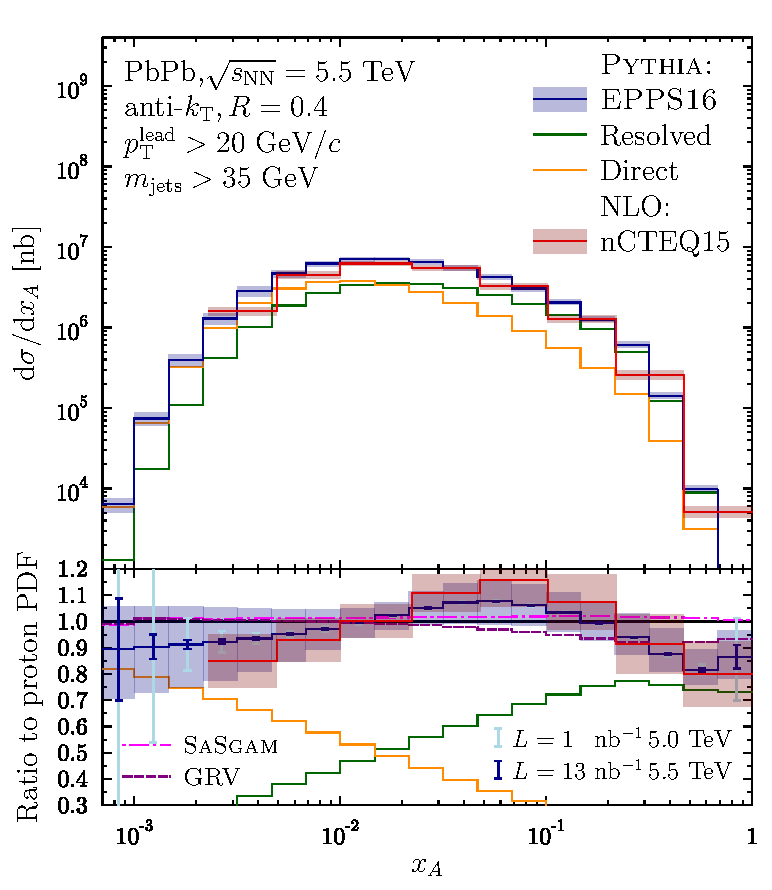
\includegraphics[width=0.49\textwidth]{\main/smallx/fig/plotxA_ATLAS.pdf}
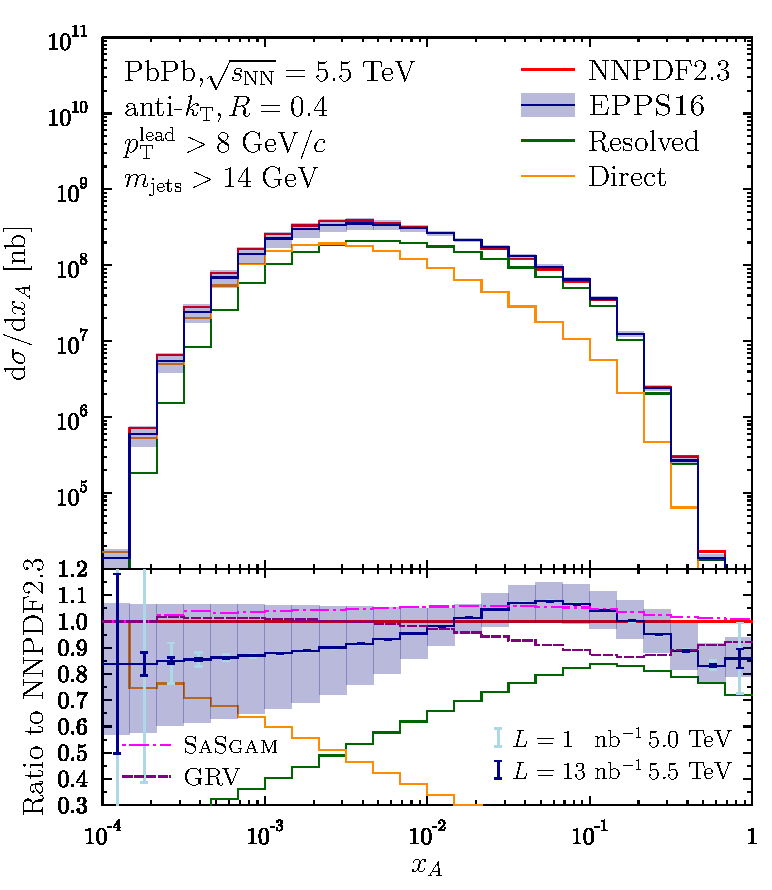
\includegraphics[width=0.49\textwidth]{\main/smallx/fig/plotxA_pTlow.pdf}
\caption{Photo-nuclear dijet cross-sections in ultra-peripheral Pb+Pb collisions at $\sqrt{s_{\mathrm{NN}}} = 5.5\UTeV$ with leading jet $\pT$ cut of $20\UGeVc$ (left) and $8\UGeVc$ (right). Results based on \textsc{Pythia} simulations are calculated with EPPS16 nuclear modification (blue) and the contributions from resolved (green) and direct (orange) photons are plotted separately. Ratio plots show also results with different photon PDF sets and the expected statistical uncertainties corresponding to the LHC (light blue) and the HL-LHC (dark blue) luminosities. Corresponding results based on NLO calculations for Pb+Pb collisions at $\sqrt{s_{\mathrm{NN}}} = 5.02\UTeV$ with nCTEQ15 nPDFs (red) are shown in case leading jet $\pT$ cut of $20\UGeVc$.}
\label{fig:UPCdijetNPDF}
\end{figure}

%Guzey, Klasen
Inclusive dijet photoproduction in UPCs can also be evaluated to the next-to-leading order (NLO) accuracy of perturbative QCD. The corresponding cross section can be written in the following form~\cite{Klasen:2002xb}:
 \begin{eqnarray}
 d\sigma(AA \to A+{\rm 2 jets}+X) = \sum_{a,b} \int dy \int dx_{\gamma} \int dx_b f_{\gamma/A}(y)f_{a/\gamma}(x_{\gamma},\mu^2)f_{b/A}(x_A,\mu^2) d\hat{\sigma}(ab \to {\rm jets}) \,,
\label{eq:cs_jets}
\end{eqnarray}
where $a,b$ are parton flavors; $f_{\gamma/A}(y)$ is the flux of equivalent photons emitted by one ion,
which depends on the photon light-cone momentum fraction $y$;
$f_{a/\gamma}(x_{\gamma},\mu^2)$ is the PDF of the photon, which depends on the momentum fraction $x_{\gamma}$ 
and the factorization scale $\mu$; $f_{b/A}(x_A,\mu^2)$ is the nPDFs with $x_A$ being the corresponding parton momentum fraction;
$d\hat{\sigma}(ab \to {\rm jets})$ is the elementary cross section for production of two- and three-parton final states emerging as jets
 in the interaction of partons $a$ and $b$. The sum over $a$ involves quarks and gluons for the resolved photon contribution 
 and the photon for the direct photon contribution dominating at $x_{\gamma} \approx 1$.
 
In Eq.~(\ref{eq:cs_jets}), the momentum fractions $x_A$ and $z_{\gamma}$ are determined by measuring the final jets:
\begin{eqnarray}
x_{A} & =& \frac{m_{\rm jets}}{\sqrt{s_{NN}}}e^{-y_{\rm jets}} \,, \quad \quad z_{\gamma}=\frac{m_{\rm jets}}{\sqrt{s_{NN}}}e^{y_{\rm jets}} \,, \nonumber\\
m_{\rm jets} &=& \left[\left(\sum_i E_i\right)^2-\left|\sum_i \vec{p}_i \right|^2 \right]^{1/2} \,, \quad \quad
y_{\rm jets}=\frac{1}{2} \ln \left(\frac{\sum_i E_i+p_{i,z}}{\sum_i E_i-p_{i,z}} \right) \,.
\label{eq:estimators2}
 \end{eqnarray}
 where  the index $i$ runs over all measured jets; $E_i$ and $\vec{p}_i$ denote the jet energy and momentum, respectively.
 Note that at the leading order (LO), the kinematics of $2 \to 2$ parton scattering, i.e., $x_A$ and $z_{\gamma}$, 
 can be exactly reconstructed from the dijet measurement.
 At NLO, Eq.(\ref{eq:estimators2}) serves as a hadron-level estimator of $x_A$ and $z_{\gamma}$
 entering Eq.(\ref{eq:cs_jets}).
 
 Figure~\ref{fig:UPCdijetNPDF}
 %\ref{fig:x_A} 
 presents predictions of Eq.~(\ref{eq:cs_jets}) for the cross section of dijet photoproduction in Pb-Pb UPCs at $\sqrt{s_{NN}}=5.02$~TeV in the ATLAS kinematics as a function of $x_A$. The red solid lines and the associated shaded band correspond to the central fit of nCTEQ15 nPDFs and their uncertainty, respectively.
 %vg; the green and orange curves give separately the resolved and direct photon contributions. 
%\begin{figure}[t]
% 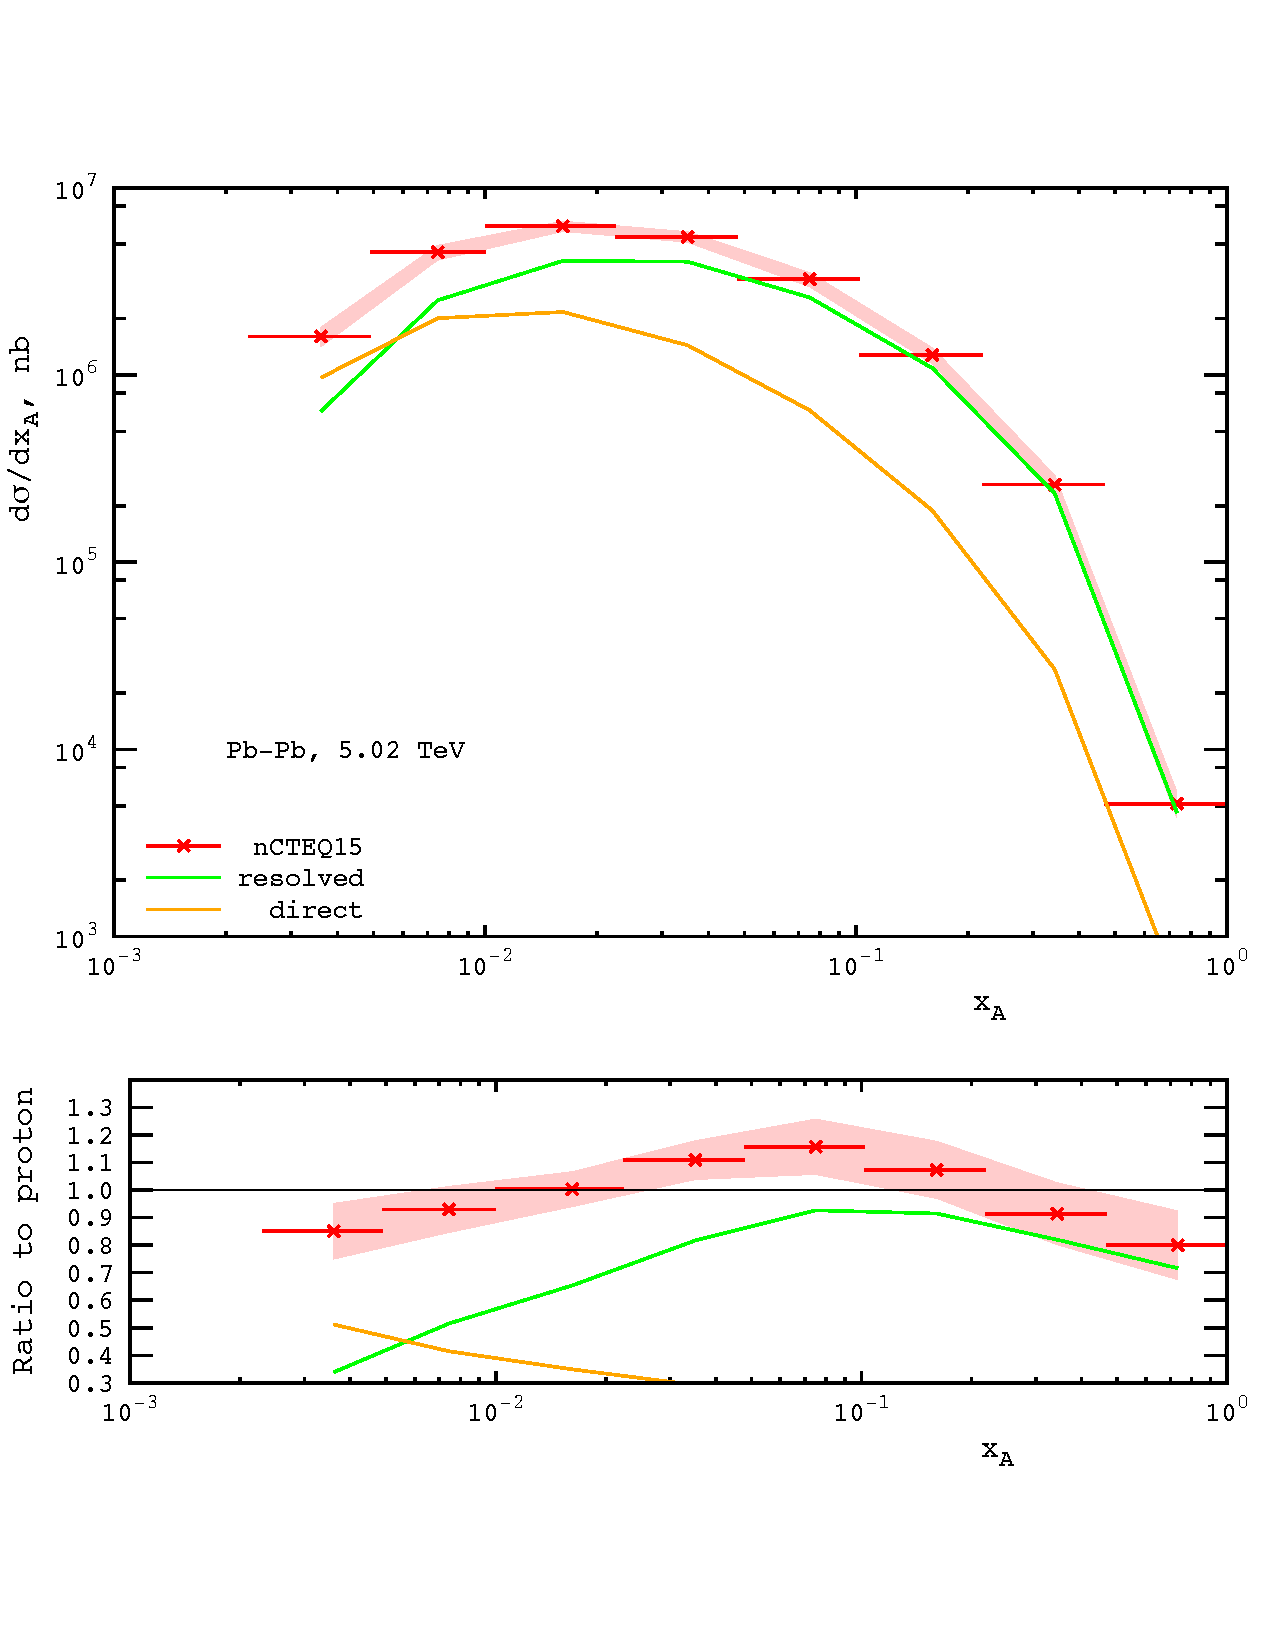
\includegraphics[scale=0.5]{smallx/fig/xA3_unc.pdf}
% \caption{The NLO pQCD cross section of dijet photoproduction in Pb-Pb UPCs at $\sqrt{s_{NN}}=5.02$ TeV 
% as a function of $x_A$ in the ATLAS kinematics. Top: The nCTEQ15 predictions (red solid points and associated error bands
% and separately the resolved (green) and direct (orange) photon contributions.
%Bottom: The ratio to the calculation with the free proton and neutron nCTEQ15 PDFs.}
% \label{fig:x_A}
%\end{figure} 
The top panel of this figure demonstrates that NLO pQCD correctly reproduces the shape and, at least 
semi-quantitatively, the normalization of the preliminary ATLAS data.  The lower panel of Fig.~\ref{fig:UPCdijetNPDF} %\ref{fig:x_A}
shows 
the ratio of the curves from the upper panel to the result of the calculation, where nCTEQ15 nPDFs are substituted by 
free proton and neutron PDFs. One can see from this panel that the central value of the ratio of the two cross sections reveals the expected trend of 
nuclear modifications of nPDFs: $20\%$ shadowing for small $x_A < 0.01$, which is followed by $~10\%$ antishadowing (enhancement)
around $x=0.1$ and then $~20\%$ suppression for $x_A > 0.3$.
Note that since the uncertainties of nCTEQ15 nPDFs are of the same magnitude as the effect of nuclear modifications, 
inclusion of this dijet data if global QCD fits of nPDFs should in principle reduce the existing uncertainty.

%vg Guzey: a few sentences on diffractive dijets on UPCs
It is also important to study diffractive dijet photoproduction
in UPCs in the reaction $A + A \rightarrow A + jet1 +
jet2 + X + A$. NLO pQCD predictions for the cross section of this process in $pp$, $pA$, and $AA$ UPCs in the LHC kinematics were made in~\cite{Guzey:2016tek}. It was shown that studies of this process on nuclei may shed some light on the mechanism of QCD factorization breaking in diffractive photoproduction and, for the first time, give access to nuclear diffractive PDFs and test their models. 

%%% end of Guzey, Klasen


\subsection{The physics of inelastic pPb collisions}
%Editors: see subparts\\
%Indicative length 6-7 pages\\
%Figures: to be discussed based on available experimental material, preference to full scale upgrade, should be balanced in terms of experiments as well as topics\\
%Tables: one large overview table for observables
\subsubsection{Experimental overview}
%Editors: Yen-Jie Lee (CMS), Marco van Leeuwen (ALICE), Zvi Citron (ATLAS), Michael Winn (LHCb)\\
%Indicative length: 1-2 pages\\
%Content: observable overview table ordered by rate including back-of-envelope calculations for stat. error if nothing else available and explanations to instrumentation (one paragraph per experiment with suitable comparison with Run1/2), short mentioning of 'far beyond' observables in terms of luminosity in same collision system as default.

%intro by MW
Collisions of protons and lead ions are an integral part of the LHC ion programme since the 2012 pilot run. In particular, within collinear factorisation, constraints on our knowledge of the nuclear wave functions could be extended by clean probes at high $Q^2$ by dijets and heavy gauge boson available for the first time in nuclear collisions~\cite{Eskola:2016oht}. Assumption-dependent insights could be gained at lower~$Q^2$ with heavy-flavour production~\cite{Kusina:2017gkz}.  In Run 3 and 4, the increased luminosities and detector upgrades  will allow to improve  the statistical precision, to extent the kinematic reach as well as the number of available processes.  We outline the detector capabilities and observables considered as focus for studies of high-energy QCD studies in view of the four experiments highlighting one specific upgrade aiming for the low-$x$ frontier. After this introduction, two theory contributions zoom on specific aspects of the future available data.  
% ALICE general first draft MvL
\begin{itemize}
\item During run 3 and 4, \textbf{ALICE} will measure heavy flavor and charged particle production at mid-rapidity in pPb (and Pbp) collisions. These measurements will constrain the parton densities in the nucleus at moderate $x$. At forward and backward rapidity, measurements of W and Z-boson production, as well as a range of quarkonia (J/$\psi$, $\psi(2S)$, and the $\upsilon$ family) will be performed. In particular the W and Z boson measurements will constrain the nuclear PDFs exemplary shown for the Z-boson in Fig.~\ref{fig:plotDY}, while the quarkonia are also sensitive to final state effects. 
%ATLAS Z. C.
\item \textbf{ATLAS}
ATLAS will measure heavy electro-weak bosons, $W$ and $Z$, with the larger pPb dataset which will be available in Runs 3 and 4.  The much larger luminosity will allow precision in these measurements significantly surpassing that which is currently available.  Projected $W$ and $Z$ boson cross sections are shown in Figure \ref{fig:ATLASWZxsection} [reference to ATLAS note when available].  Previous results have suggested that the modification of EW boson cross sections that is described with nPDFs, appears to be stronger in more central collisions \cite{Aad:2015gta,TheATLAScollaboration:2015lnm}.  Figure \ref{fig:ATLASWZcent} (left) shows the projected boson yield ratio of central to peripheral collisions, $R_{\mathrm{CP}}$, for different centrality bins.  The right panel of Figure \ref{fig:ATLASWZcent} shows the yield of $Z$ bosons scaled by the nuclear thickness function, T$_{\mathrm{AB}}$,  as a function of centrality, and indicates the favorable comparison of the yield uncertainties with the uncertainty of T$_{\mathrm{AB}}$.
%CMS E. C.
\item  Using the larger pPb dataset available during Runs~3--4, \textbf{CMS} will further improve the precision on differential measurements of W and Z bosons (constraining quark and antiquark nPDFs), as well as dijet and $t\overline{t}$ production (gluon nPDFs). While first Run~2 results on W boson production already feature experimental uncertainties smaller than the nPDF ones, the larger luminosity by a factor 5 to 10 expected in Runs~3--4 will allow for another large jump in the constraints on nPDFs from data. In addition, novel studies will become possible, such as the measurement of differential $t\overline{t}$ distributions (CMS projection expected soon), for an improved constraining power on nPDFs, as well as the mass dependence of Drell-Yan production down to the $\PGU$ meson mass region. Heavy flavour meson cross sections will also be measured, which are sensitive to low-$x$ gluon nPDFs: D mesons ($\pT>0.5$\,GeV), B mesons ($\pT>5$\,GeV), prompt and nonprompt $J/\psi$ ($\pT>3$\,GeV), and $\Upsilon(n)$ down to $\pT=0$. 
\todo{ references to projection plots, to be done \ref{fig:CMShighpt}}
%LHCb draft MW
\item In \textbf{LHCb} during Run 3 and 4, the average charged particle multiplicity in $p$Pb and Pb$p$ collisions will be smaller than the nominal conditions in pp running with an average  pile-up of 5 interactions. The low rates in pPb collisions allow to process the complete inelastic rate in the HLT. Hence, LHCb can fully profit from the luminosity increase including $\pT=0$ heavy-flavour production.  A natural focus is the study of open and hidden beauty and charm production with improved precision. A new focus of LHCb, profitting from the increased luminosity, is the study of W,Z and in particular Drell-Yan down to low masses production at forward rapidity. Direct photon studies in the conversion channel will strongly profit from the increased luminosity. \todo{put proper references to plots}
\end{itemize}

%\begin{table}[htbp]
% {\footnotesize
%\centering
%\begin{tabular}{|c|c|c|c|}
%\hline
% Observable & $p_{T}$[GeV/$c$]-range, mass & $y_{lab}$              & %precision where available \\
%\hline
%ALICE   &  &   &  \\
%        W                &          & [-4.4,-3] [2,3.5] & 6-8\% (syst)
%\\
% Z                &          & [-4.2,-3] [2,3.5] &  3-4\%  (syst)  %    \\
%\hline
%ATLAS                    &          &        &                     %        \\
%         $\gamma$                 & $\ET>25$~\UGeV  &  $-2.02\eta_{cms}<1.1$      &                    
%\\
%MW taken from https://atlas.web.cern.ch/Atlas/GROUPS/PHYSICS/CONFNOTES/ATLAS-CONF-2017-072/
%        W                 &          &     -2.965$<\eta_{cms}<2.035$   &                    
%\\
%MW taken from projection kinematics
%         Z                 &  $ -5<y_{cms}<5 $        &        &    \\
%         top                 &           &        &                    
%\\
%taken from projection kinematics
%\hline
%CMS                      &          &        &                             \\
%          low-mass Drell-Yan               &          &        &                    
%\\
%To be completed by CMS
%         W                &          &     -2.5$<\eta_{cms}<2.5$    &                    
%\\
%MW from https://arxiv.org/pdf/1503.05825.pdf

 %         Z               &          &     -2.0$<\eta_{cms}<2.0$    &                    
%\\
%MW from https://arxiv.org/pdf/1512.06461.pdf, can be certainly expanded...
%          Dijets               &          &  -3.0$<\eta_{cms}<3.0$      &                    
%\\
% MW roughly taken from projection plot
%         top                 &           &        &      \\
%\hline
%LHCb                           &         &                    &         \\

%         $D\bar{D}$-correlations     & $\pT(D)>0$~\UGeVc & 1.5>y$^{cms}$(D)>4.0 -5.0>y$^{cms}$(D)>-2.5       &                      \\
%       &  open-charm production     &          &        &                     \\
%   open-beauty production      &  $\pT(B)>0$~\UGeVc & 1.5>y$^{cms}$(B)>4.0 -5.0>y$^{cms}$(B)>-2.5              &                     \\
%&  $\gamma$     &  &        &                     \\
%  low-mass Drell-Yan   &  m>$5$~\UGeVc$^2$        &    1.5>y$^{cms}$>4.0 -5.0>y$^{cms}$>-2.5      &                   
%\\
%  W     &          &   1.5>$\eta^{cms}$>4.0 -5.0>$\eta^{cms}$>-2.5      &                     \\
%  Z     &          &   1.5>y$^{cms}$>4.0 -5.0>y$^{cms}$>-2.5                      
%\\
%\hline
%\end{tabular}
%\caption{Selection of accessible observables and their acceptance for the different LHC experiments.}
%\label{tab:pPb}
%}
%\end{table}

\subsubsection{Forward calorimeter upgrade of ALICE}
%Author: Marco van Leeuwen
%1 page

The ALICE collaboration is considering to add a high-granularity forward calorimeter (FOCAL) to the experiment to  measure direct photon production in the rapidity range 3.0--5.0 and at low \pT, to probe the gluon density in protons and nuclei at $x\sim 10^-5$ where gluon saturation and non-linear effects in the gluon density may become apparent. The FOCAL design is based on the Si-W calorimeter technology, with two or three high-granularity layers with silicon pixel sensors that allow to separate electromagnetic showers with only a few mm distance between them. This unique high granularity makes it possible to reconstruct neutral pions in the forward direction and to reject the decay photon background for the direct photon measurement.

\begin{figure}
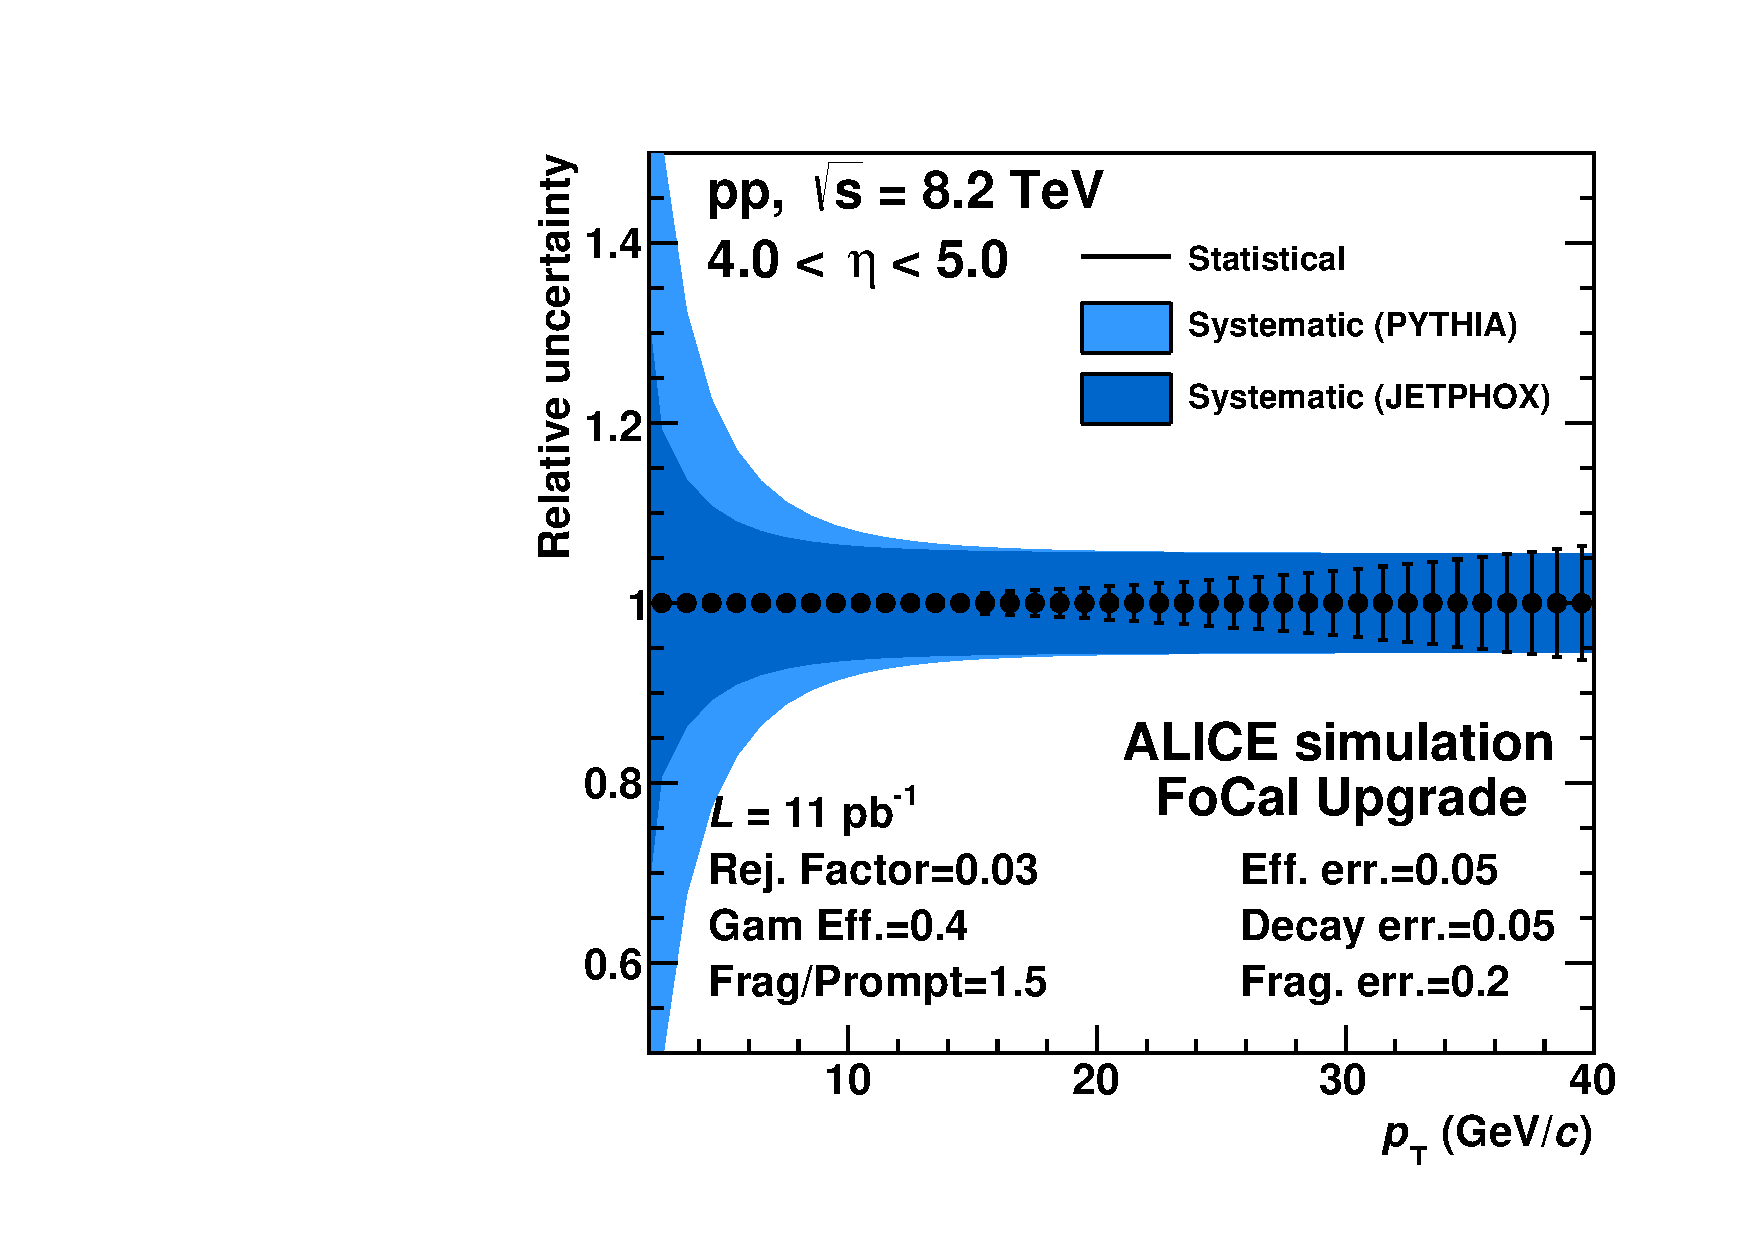
\includegraphics[width=0.5\textwidth]{\main/smallx/fig/gamma_unc_pPb_8TeV16_4eta5.pdf}
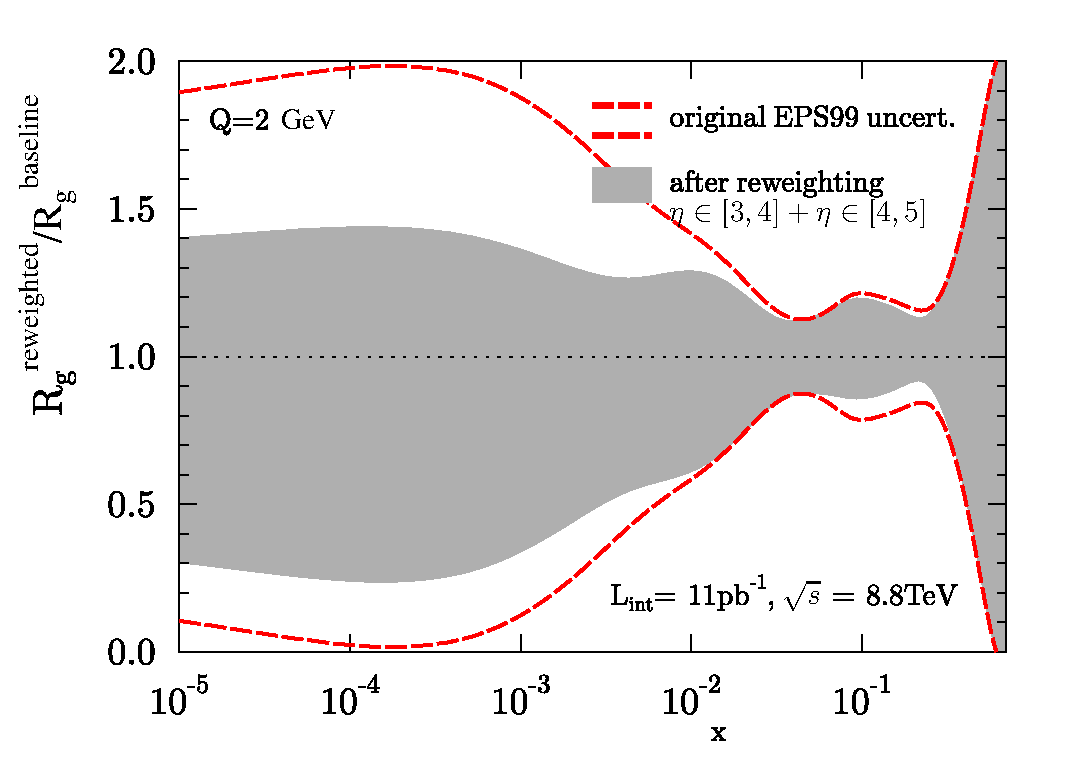
\includegraphics[width=0.5\textwidth]{\main/smallx/fig/Gluons_FOCAL_norm_2_y34_y45.pdf}
\caption{\label{fig:focal}Left panel: Projected uncertainties for the forward direct photon measurement with the ALICE FOCAL upgrade. Right panel: Uncertainty on the modification ratio of the gluon density in the Pb nucleus from a fit to FOCAL pseudo-data. The red lines show the current uncertainty and the grey band shows the uncertainty after including the FOCAL pseudo-data.}
\end{figure}

Figure \ref{fig:focal} shows the expected performance of the FOCAL detector for the direct photon measurement in p--Pb collisions. The left panel shows the projected uncertainties, which are 7-8\% at high $p_{T}$ and increase at lower momentum due to the combinatorial background. The right panel shows the impact of the measurement on our knowledge of the nuclear modification of the gluon distribution; the red lines show the current uncertainty, based on the EPS99 nPDFs, but using a broader set of parametrisation for the nuclear PDFs at the initial scale $Q_0$, similar to~\cite{Aschenauer:2017oxs}. The grey band shows the uncertainty after including the FOCAL pseudo-data. The improvement in the uncertainty is about a factor~2, but it should be noted that the direct photon measurements probes the gluon distribution at low $x$ directly, while the most of the existing data only probe $x \gtrsim 10^{-3}$ (see Fig. \ref{fig:smallx1}). At present, the only measurements that probe the very low $x$ region for nuclear PDFs are forward heavy flavour measurements from LHCb \cite{Aaij:2017gcy,Aaij:2017cqq} and ALICE \cite{Acharya:2017hdv}; theoretical developments are under way to use these data to constrain the PDFs~\cite{Kusina:2017gkz,Helenius:2018uul}. The FOCAL program will probe smaller $x$ which are produced a different process (quark-gluon compton scattering vs gluon fusion) and therefore also test universality and factorisation in this regime. Future measurements of Drell-Yan production in LHCb, as shown in Fig.~\ref{fig:DYRpPb}, will also probe this region, but will have a weaker impact for gluons at small $Q^2$ according to current experimental uncertainty estimates. 

In addition to the inclusive direct photon measurement, the FOCAL program will measure on forward $\pi^{0}$ production in pp, p-Pb and Pb-Pb collisions, which also provides important constraints for the nuclear PDFs and parton energy loss in Pb-Pb collisions at large rapidity. Correlation measurements of neutral pions and photons will be used to further probe the gluon density and to search for evidence of multiple-gluon interactions which are expected to be important in the high gluon density of the Color Glass Condensate \cite{Kharzeev:2004bw,vanHameren:2014lna}.

%\subsubsection{Detailed projections}
%Editors: experimental contacts from overview unless other contact given, description as short as possible with reference to publicly available material, to be linked to overview text and to theory parts, plots to be combined in multi-panel after being available \\
%Indicative length: 2 pages \\
%Content: W,Z(ATLAS/CMS), Drell-Yan(CMS/ATLAS), dijet(CMS/ATLAS)\\
%top (CMS/ATLAS), plot will be shown in extra part by David and Hannu \\
%W,Z,low-mass Drell-Yan (LHCb), gamma separate since new Hardware (ALICE) \\
%MW proposal plots: Dijets by CMS; W,Z by ATLAS/CMS (one triple differential from ATLAS)\\
\begin{figure}[htb]
\centering
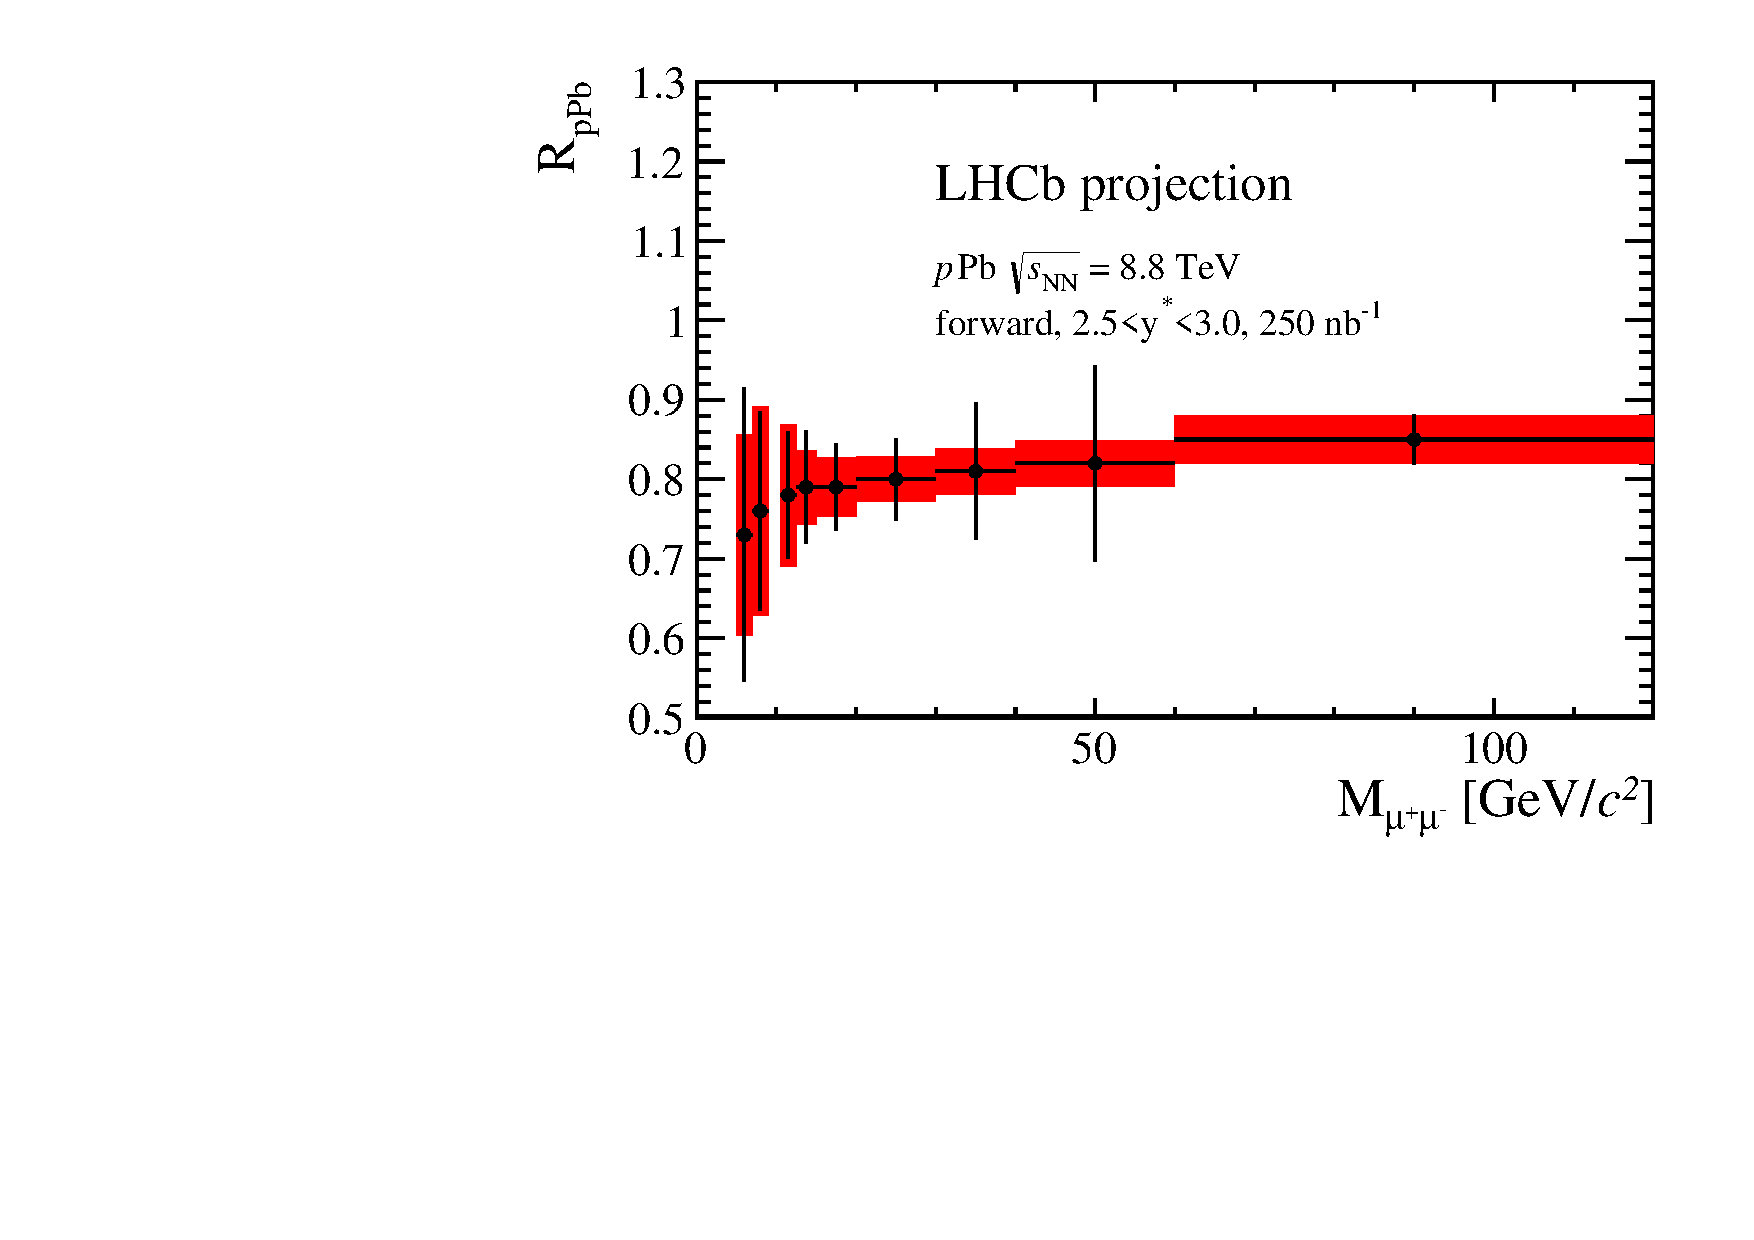
\includegraphics[width=0.49\textwidth]{\main/smallx/fig/DY_rap2_pPb.pdf}
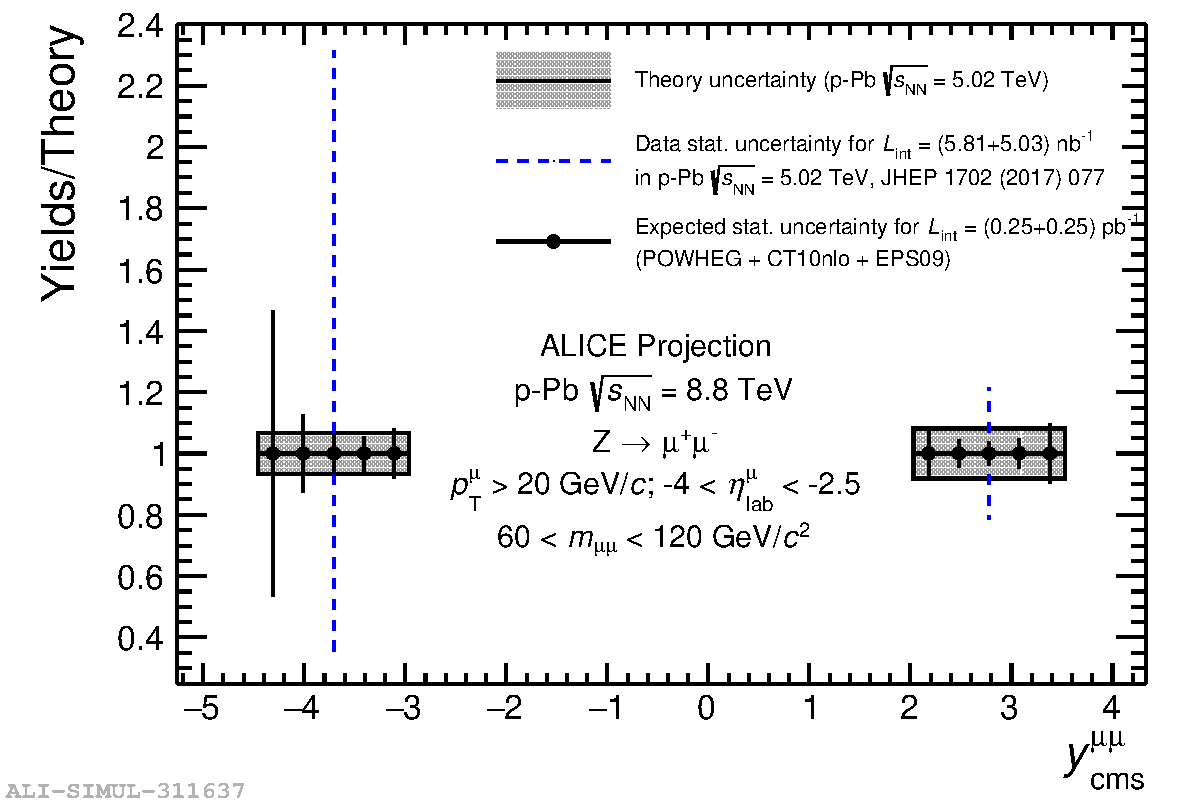
\includegraphics[width=0.49\textwidth]{\main/smallx/fig/2018-10-15-2018-10-15-z_proj_run3_pPb_statErr.pdf}
\caption{Left: $R_{pA}$ for Drell-Yan production in $2.5<y_{cms}<3.0$, one of five bins accessible with LHCb. Right: Expected statistical significance of the Z boson rapidity distribution for p-Pb collisions at $\sqrt{s_{\rm NN}} = 8.8$~TeV in run 3-4 assuming an integrated luminosity of 0.25/pb (0.25/pb) obtained with the proton (Pb ion) going toward the muon spectrometer. In the estimation, a conservative detector efficiency of 70\% is used. The results are compared with the statistical significance of the published data collected in p-Pb collisions in 2013.}
\label{fig:plotDY}
\end{figure}



%%% Dijet pseudorapidity projections %%%
%%%%%%%%%%%%%%%%%%%%%%%%%%%%%%%%%%%%%%%%
\begin{figure}[t] %%%%%%%%%%%%%%%%%%%%%%
\centering
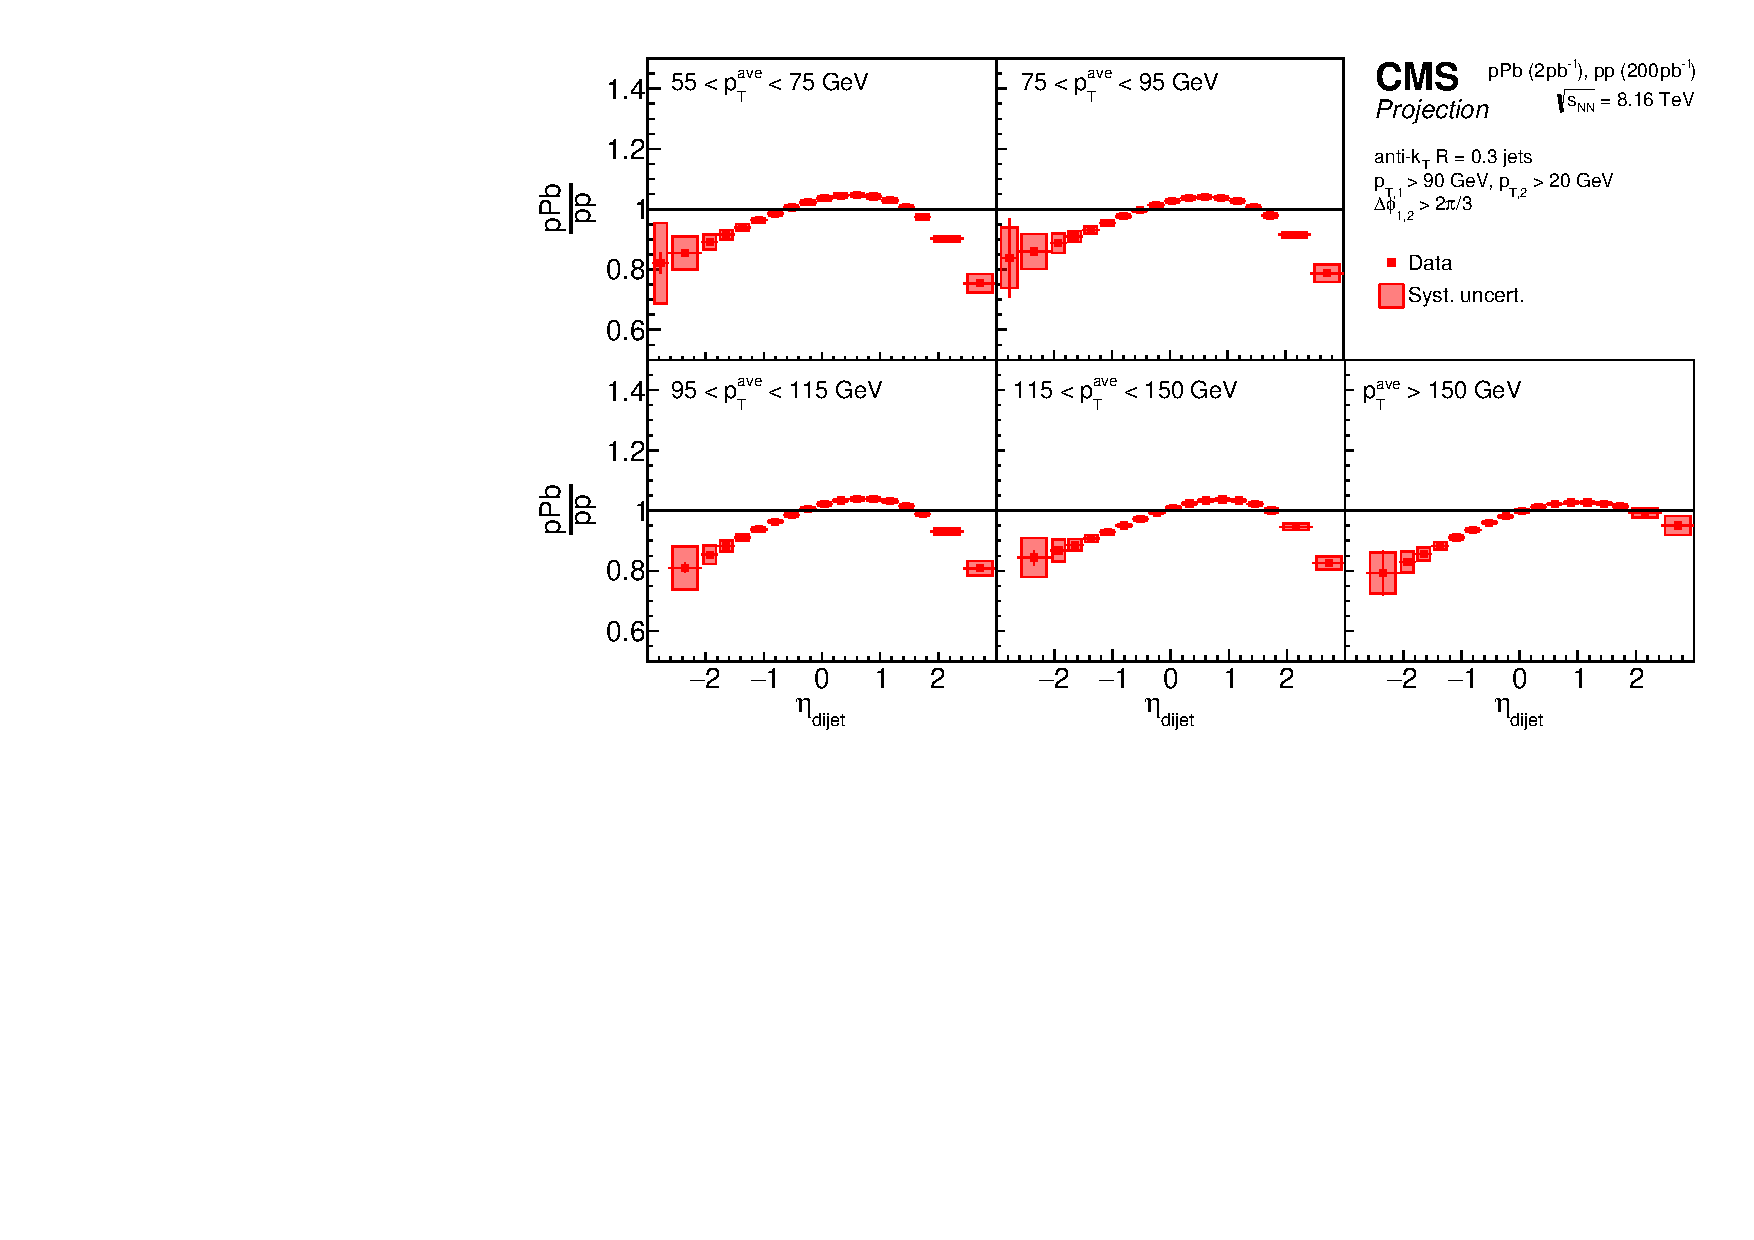
\includegraphics[width=0.96\textwidth]{\main/smallx/fig/dijet-eta-projections.pdf}
\caption{
Projected dijet $\eta$ measurements in pPb collisions with combined Run 3 and Run 4 data.
\label{fig:dijet-eta-projection-cms}
}
\end{figure}
%%%%%%%%%%%%%%%%%%%%%%%%%%%%%%%%%%%%%%%%%%%%


%%% CMS W/Z projections %%%
%%%%%%%%%%%%%%%%%%%%%%%%%%%%%%%%%%%%%%%%
\begin{figure}
    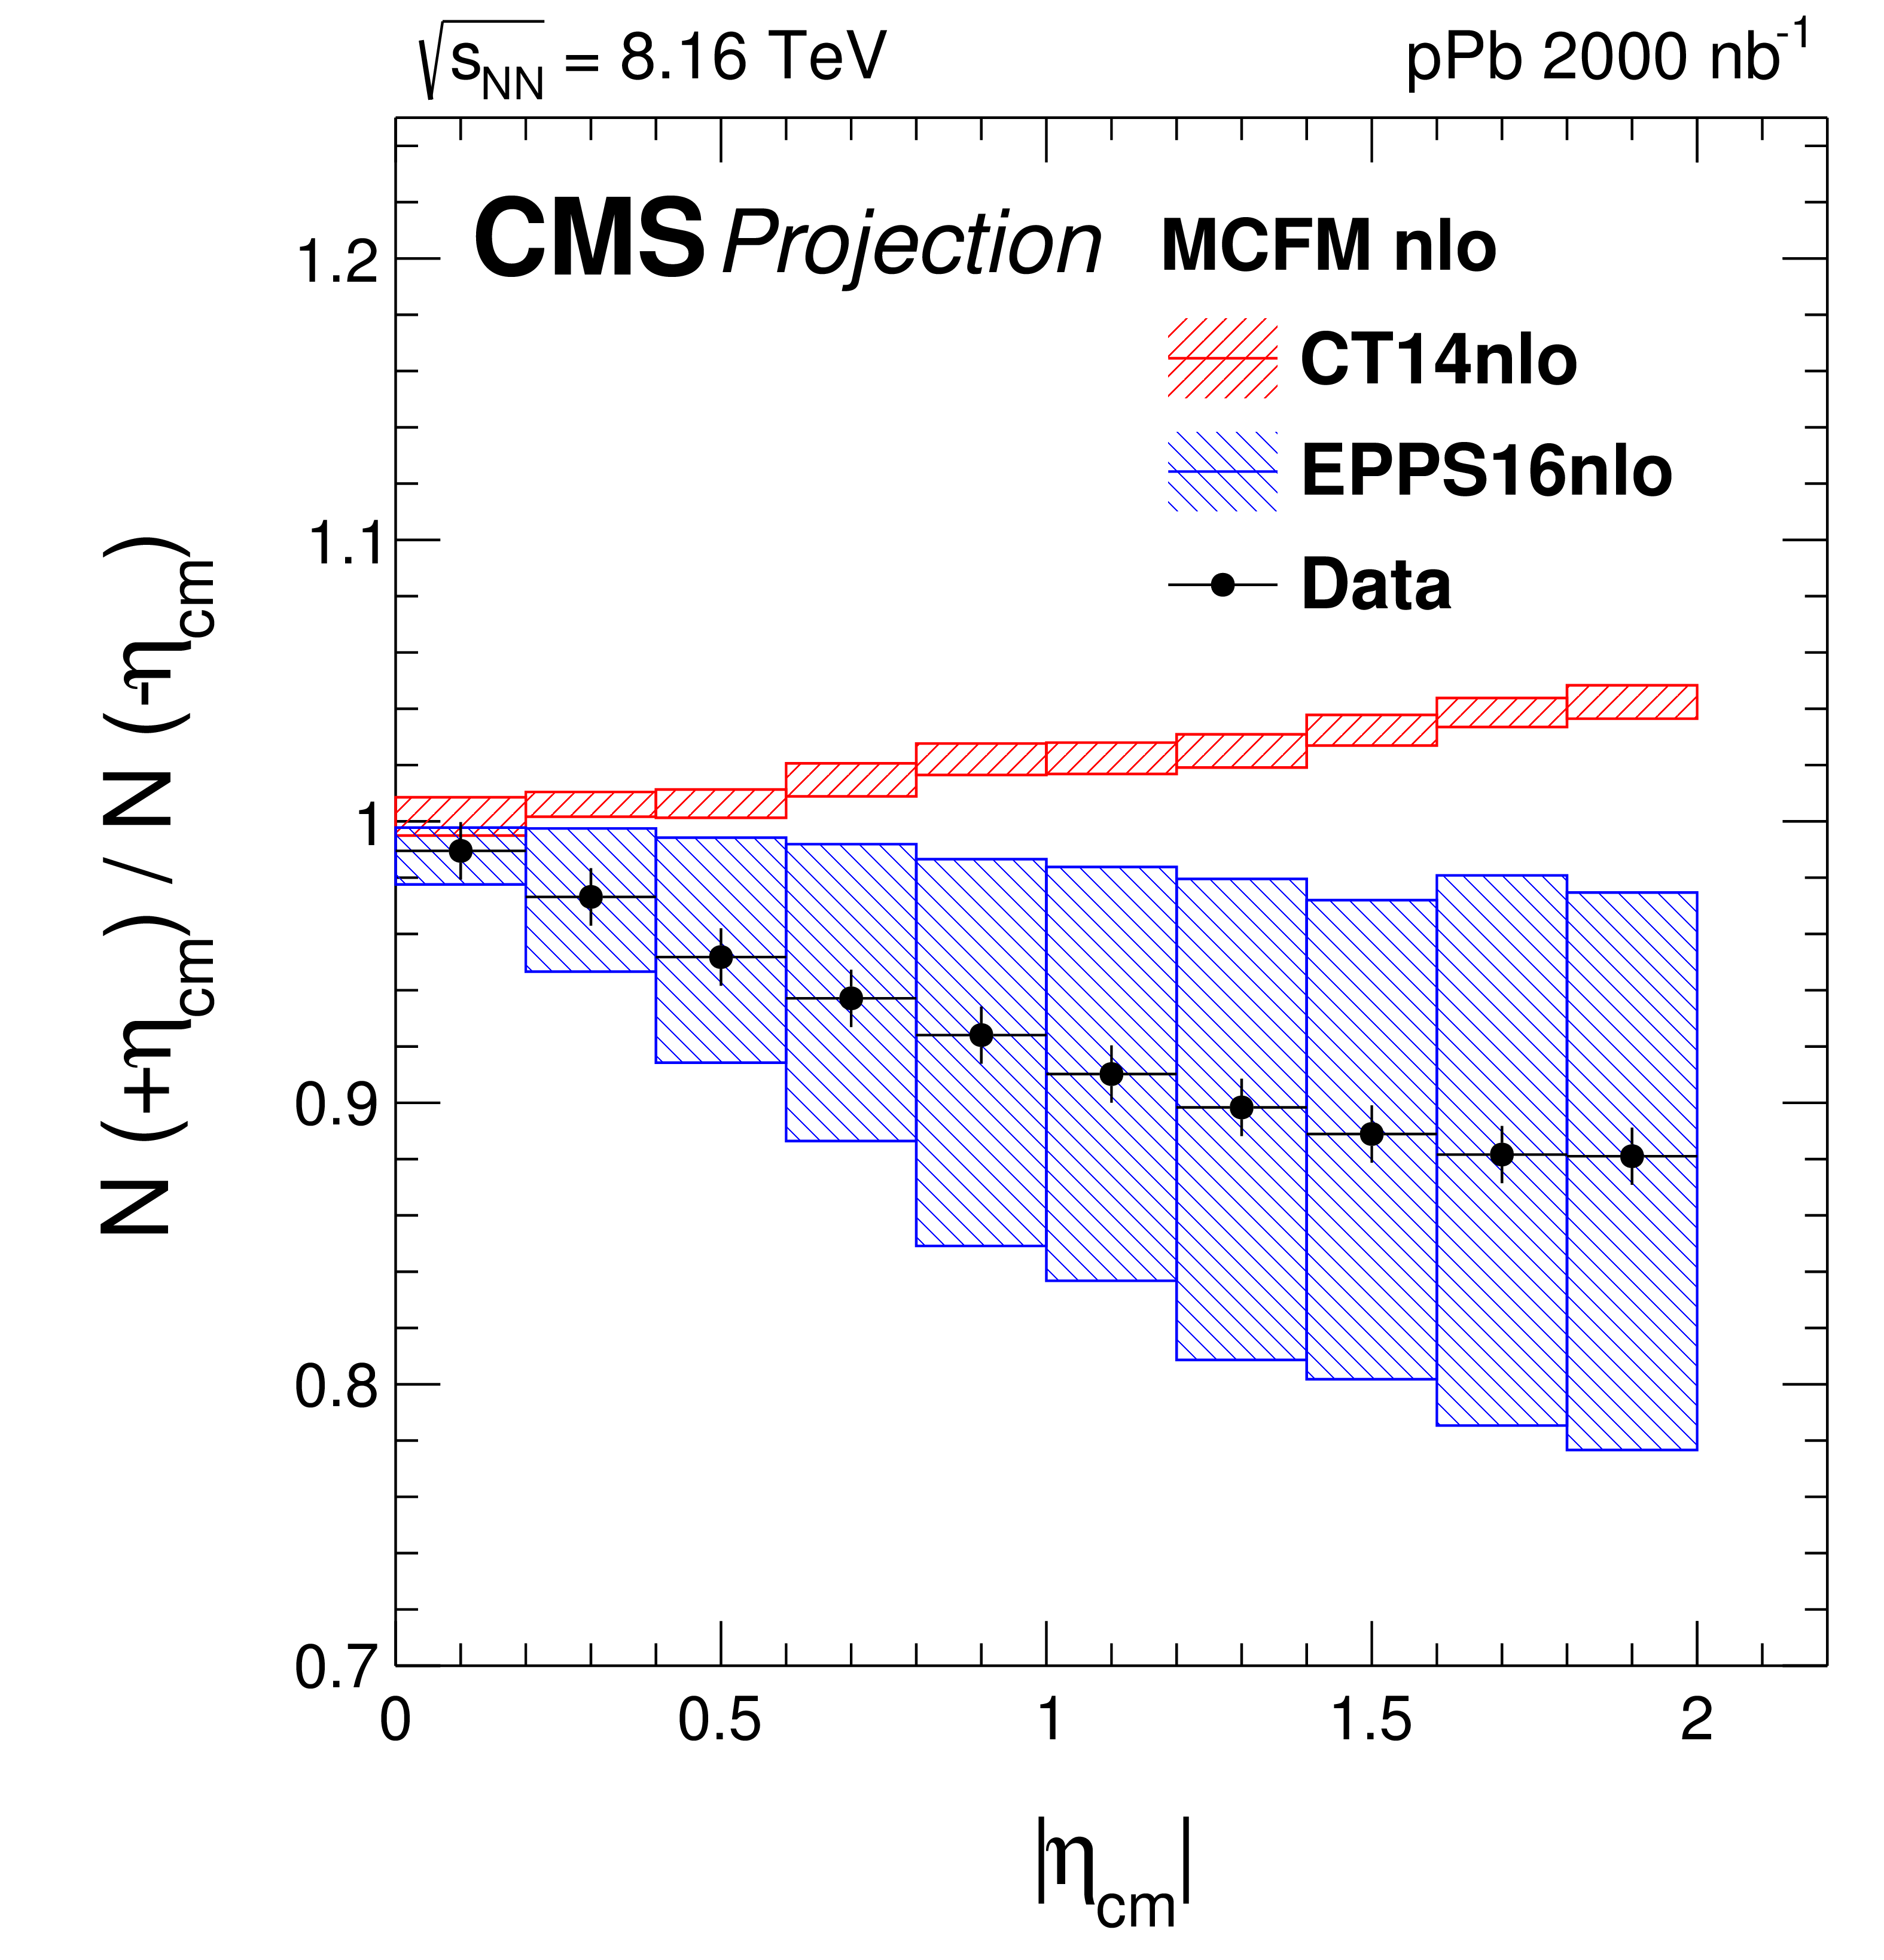
\includegraphics[width=0.46\textwidth]{\main/smallx/fig/CMS-PAS-FTR-17-002_Figure_009.png}
    \caption{Caption W-asymmetry and top production\textcolor{red}{top to be putted}
    \label{fig:CMShighpt}
    }
\end{figure}

%%% ATLAS W/Z projections %%%
%%%%%%%%%%%%%%%%%%%%%%%%%%%%%%%%%%%%%%%%
\begin{figure}
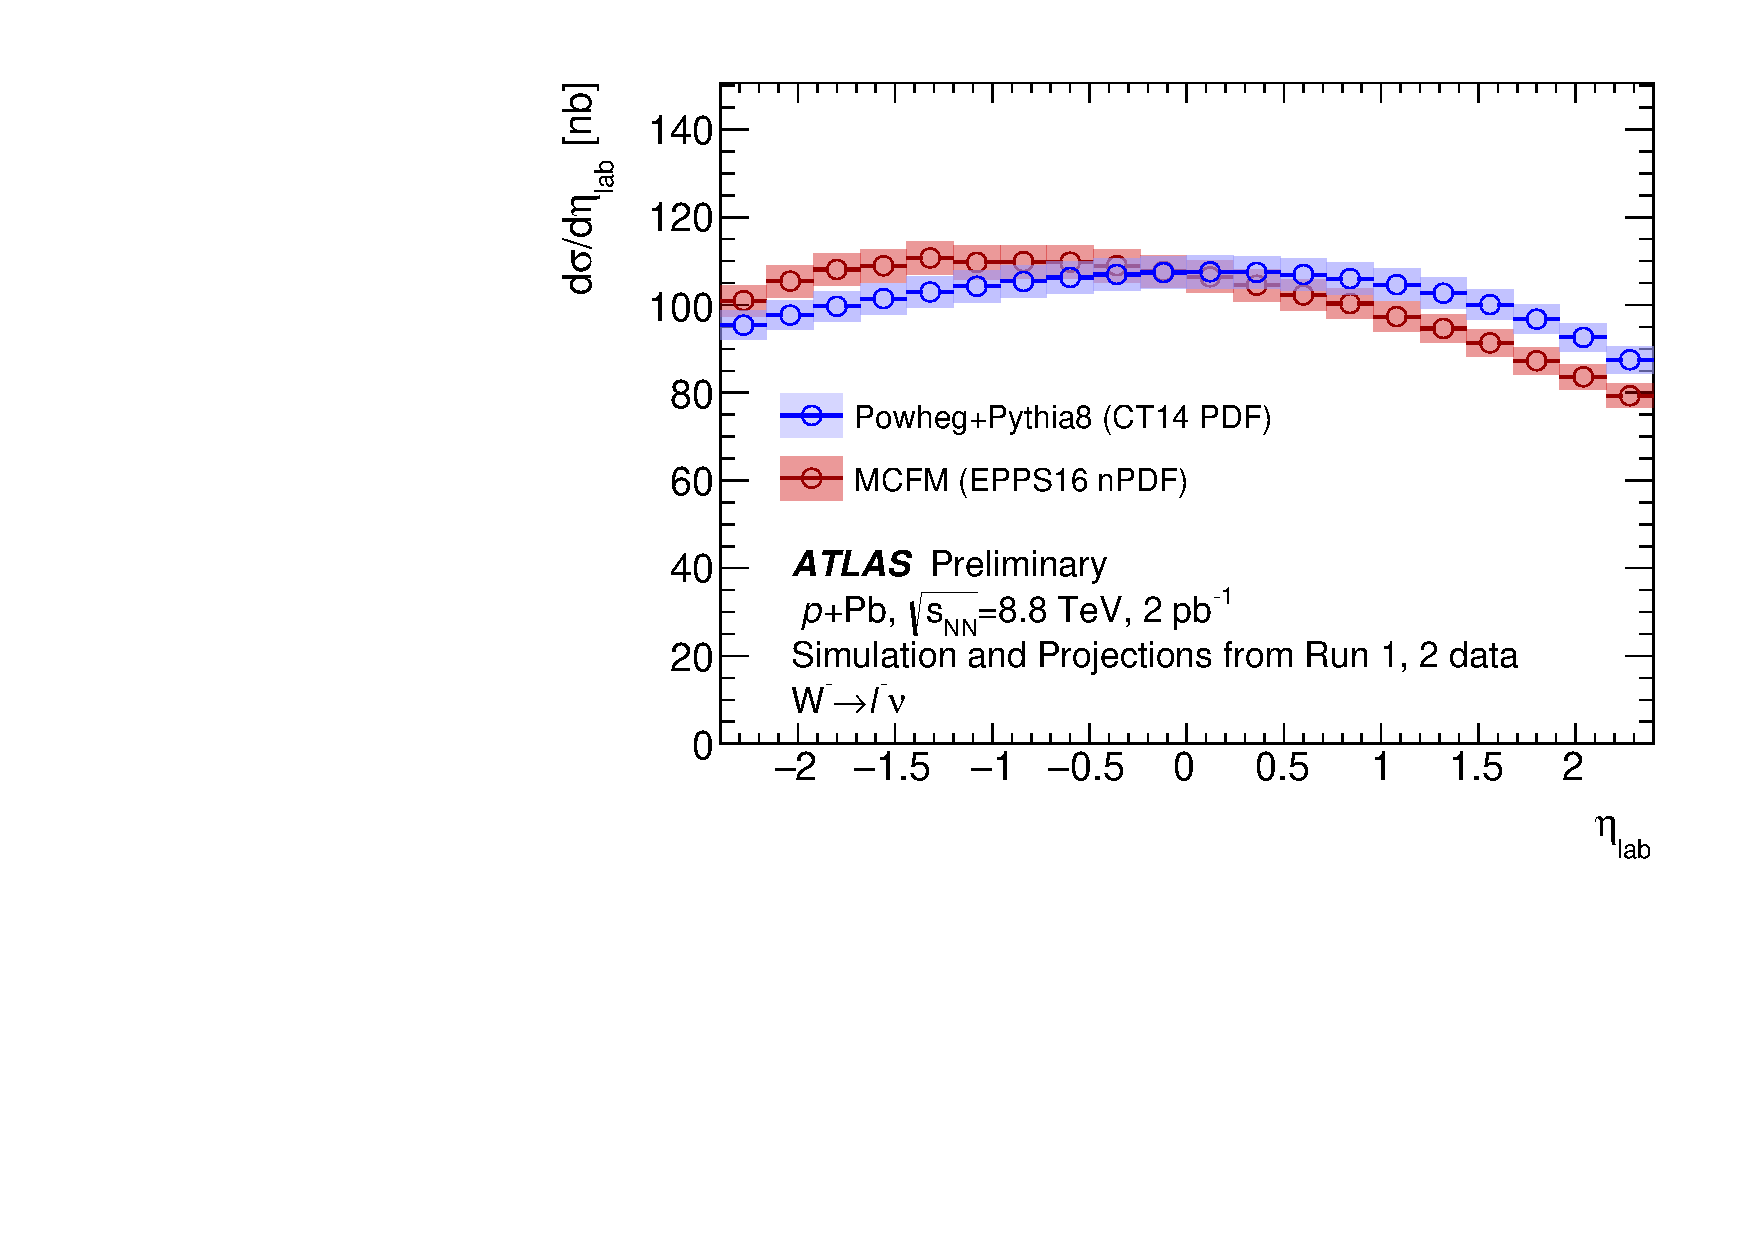
\includegraphics[width=0.49\textwidth]{\main/smallx/fig/Wminus_8p8TeV_eta_fid_2000nb.pdf}
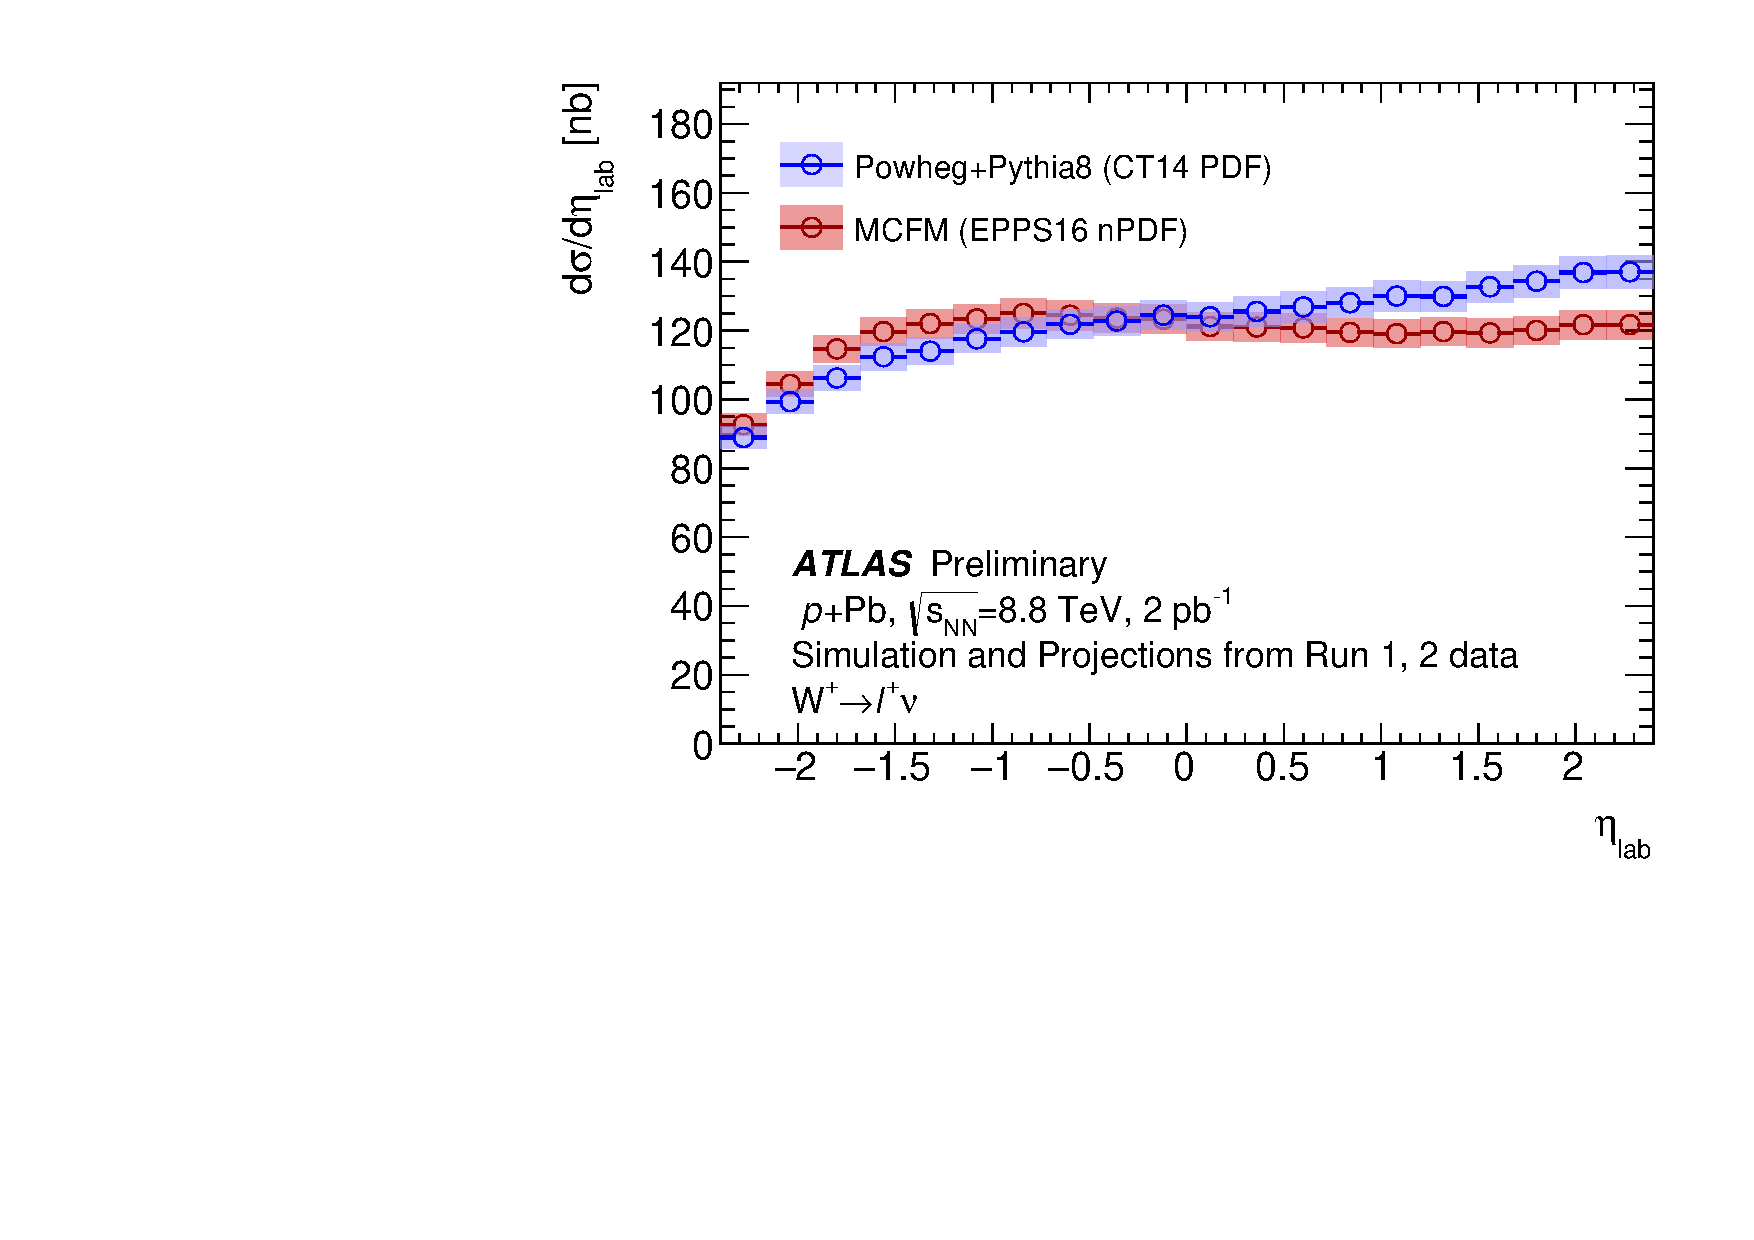
\includegraphics[width=0.49\textwidth]{\main/smallx/fig/Wplus_8p8TeV_eta_fid_2000nb.pdf}\\
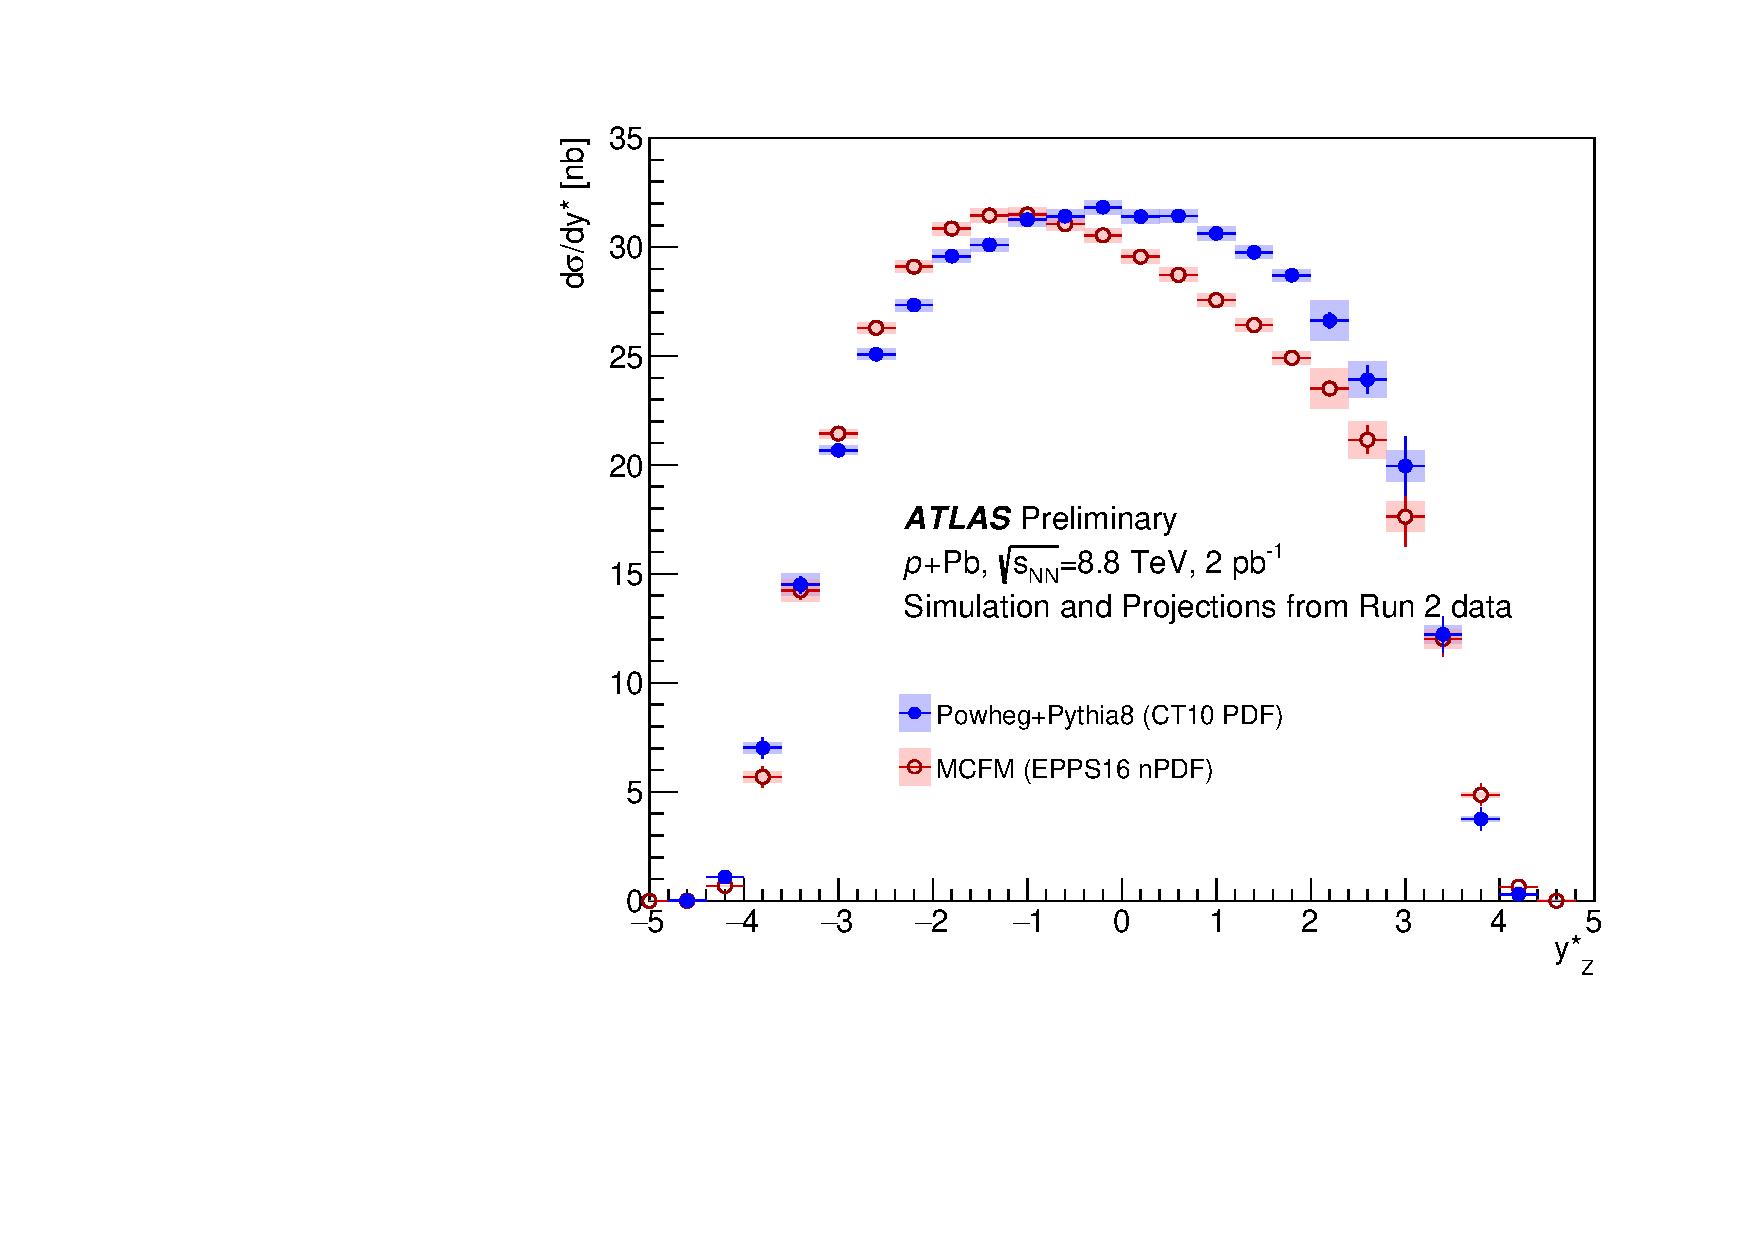
\includegraphics[width=0.49\textwidth]{\main/smallx/fig/Zprojection_xsy.pdf}
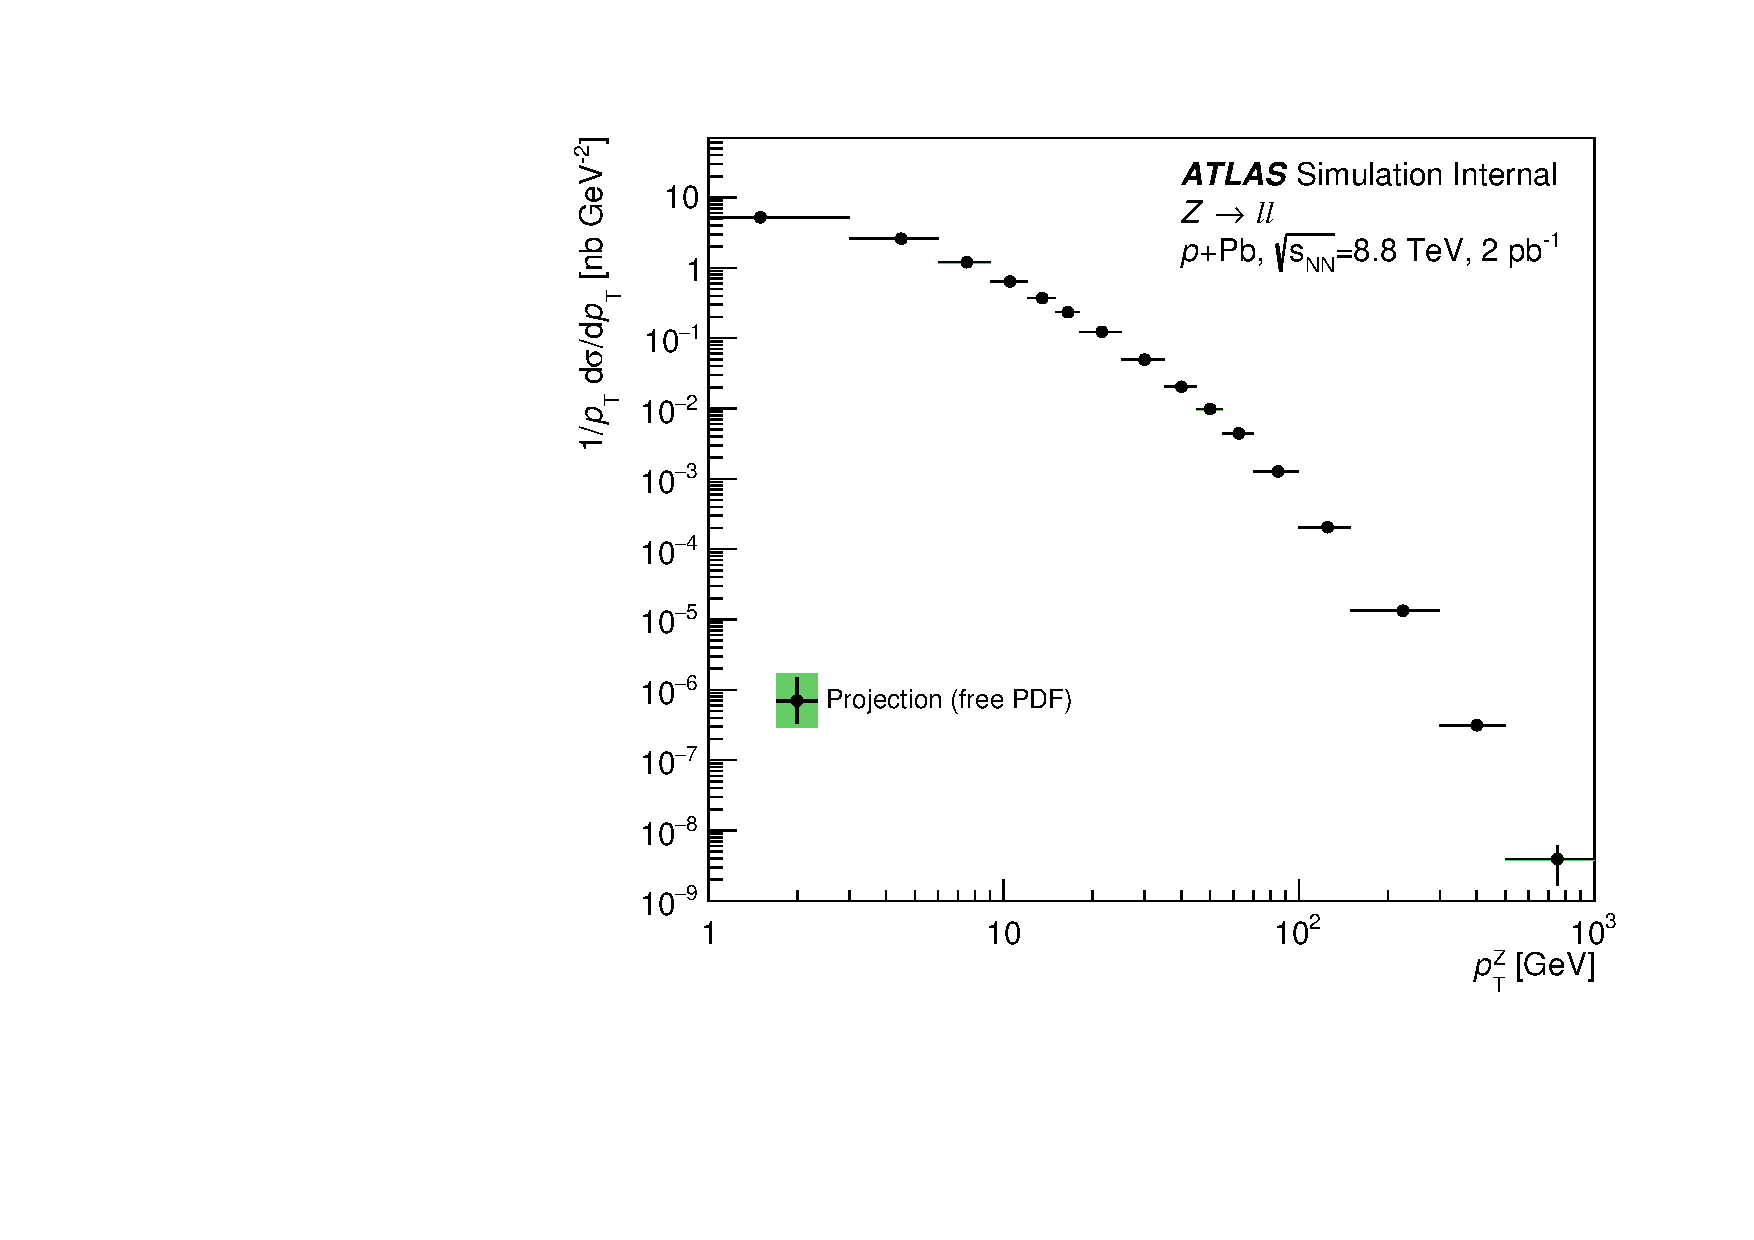
\includegraphics[width=0.49\textwidth]{\main/smallx/fig/Zpt_projection.pdf}
\caption{Top row:Fiducial cross-sections for $W^+$ (left) and $W^-$ (right) boson production in pPb collisions at $\sqrt{s_\mathrm{NN}}=8.8$~TeV differential in the charged lepton pseudorapidity measured in the laboratory frame $\eta_\mathrm{lab}$. The cross-sections are projected with nuclear effects described by the EPPS16 nPDF set and without any nuclear effects. The boxes represent the projected total uncertainties (quadratic sum of statistical and systematic uncertainties), while vertical bars represent statistical uncertainties (smaller than the marker size).
Botton row: $Z$ boson rapidity (left) and transverse momentum (right) differential cross sections.\textcolor{red}{to be updated w/final}}
\label{fig:ATLASWZxsection}
\end{figure}


\begin{figure}
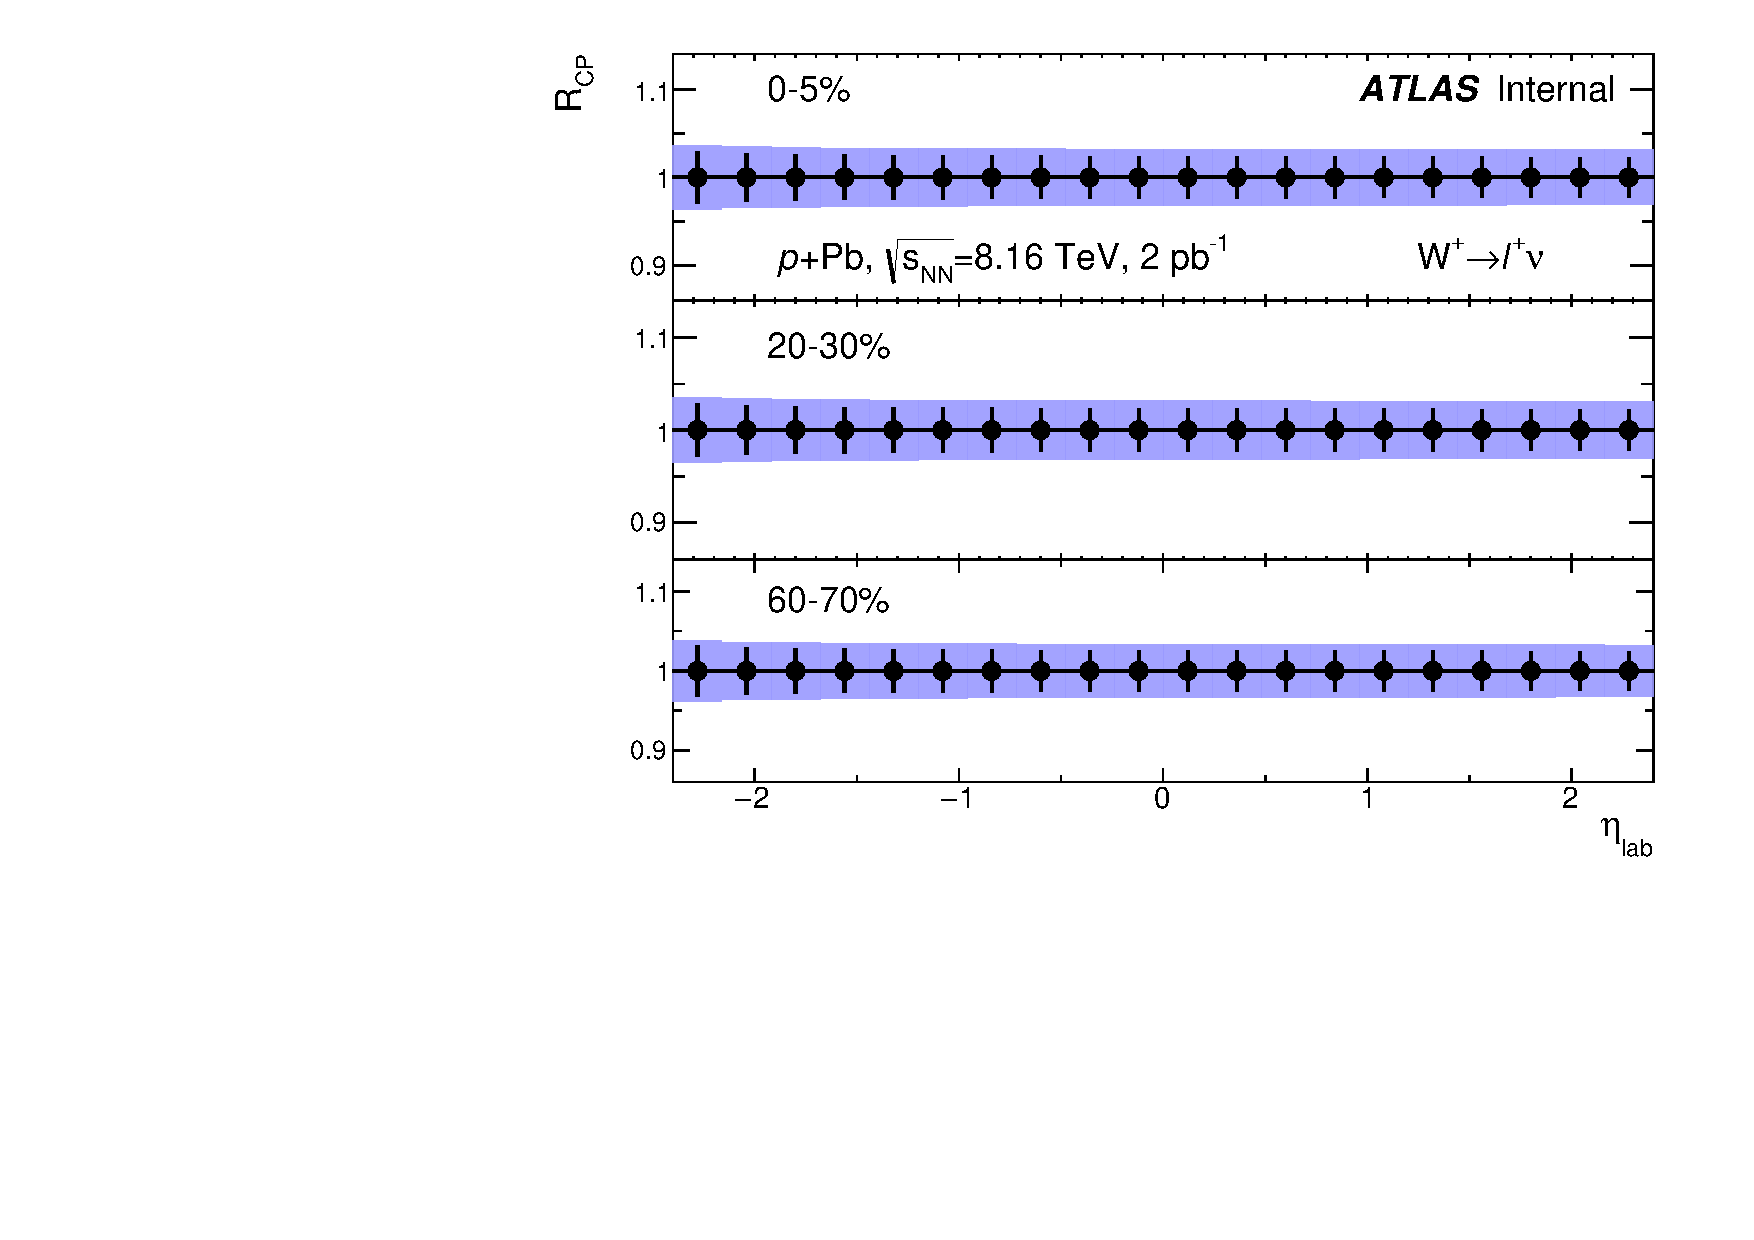
\includegraphics[width=0.49\textwidth]{\main/smallx/fig/Wplus_RCP_2000nb.pdf}
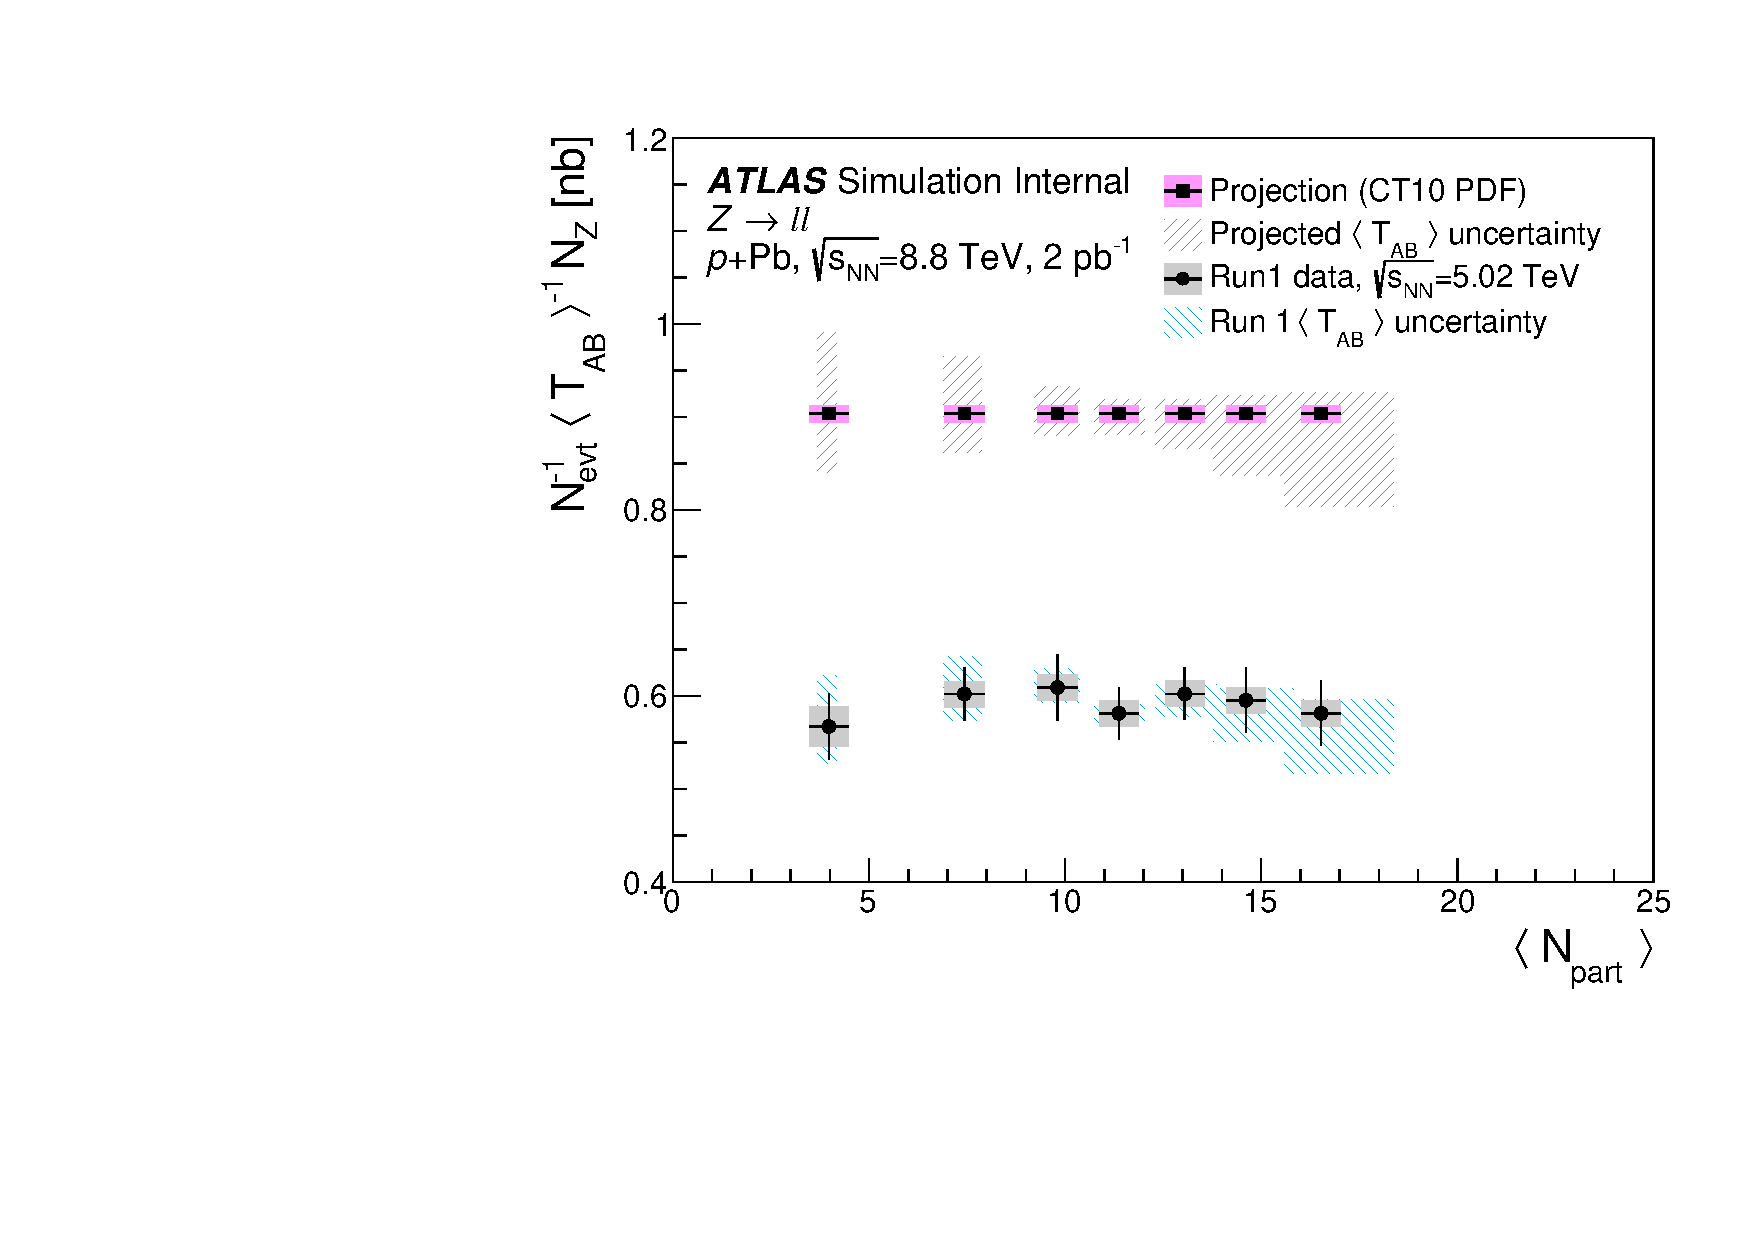
\includegraphics[width=0.49\textwidth]{\main/smallx/fig/Zprojection_cent.pdf}
\caption{Left:Uncertainties on measurments of the $W^+$ (left) and $W^-$ (right) boson yield ratio of central to peripheral collisions $R_\mathrm{CP}$.  The boxes represent the projected total uncertainties (quadratic sum of statistical and systematic uncertainties), while vertical bars represent statistical uncertainties.  Right:Projected $Z$ boson yields scaled by T$_{\mathrm{AB}}$ as a function of the number of nucleon participants.  Statistical uncertainties are everywhere smaller than the marker size, and projected systematic uncertainties (green) are described in the text.  The projections are compared with a previous run 1 analysis  \cite{Aad:2015gta}.\textcolor{red}{to be updated w/final}}
\label{fig:ATLASWZcent} 
\end{figure}

%%%%%%%%%%%%%%%%%%%%%%%%%%%%%%%%%%%%%%%%%%%%

\begin{figure}
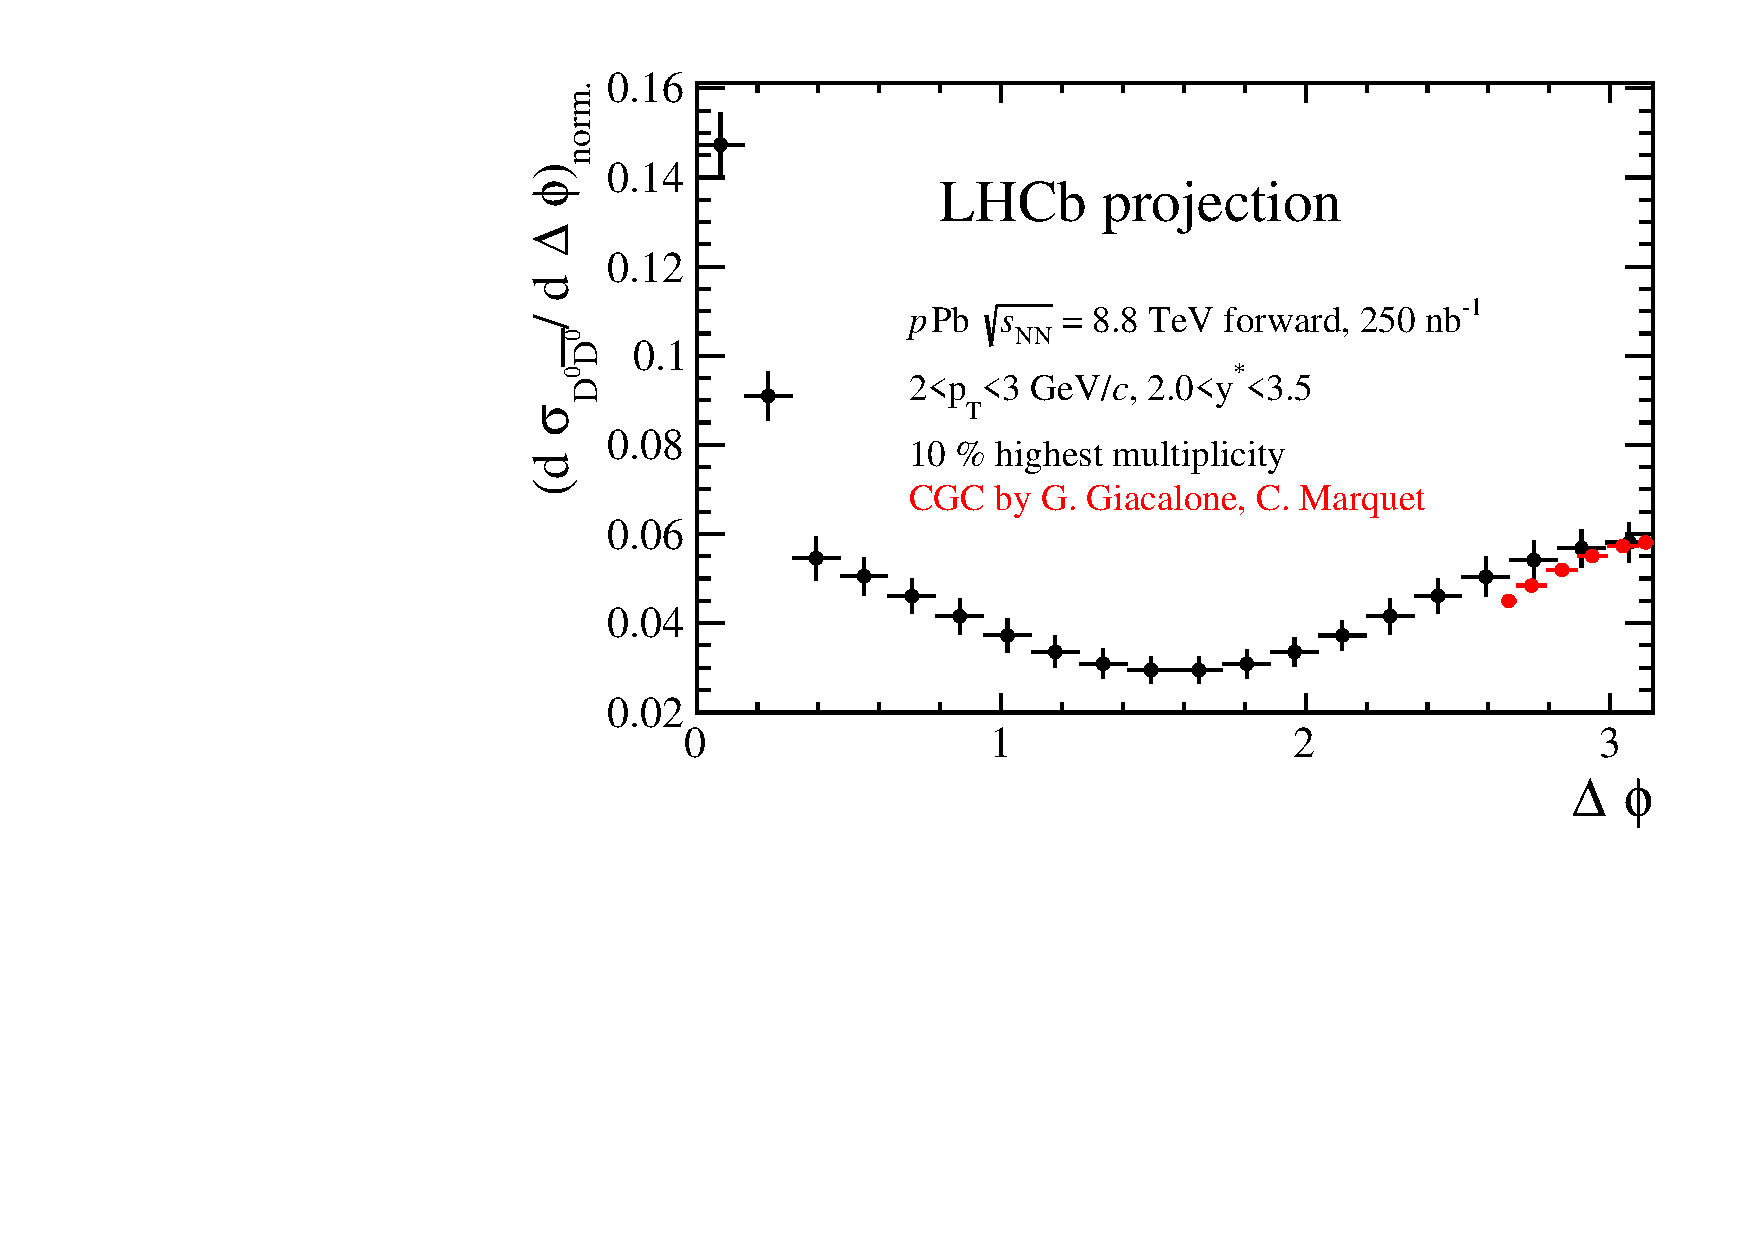
\includegraphics[width=.5\textwidth]{\main/smallx/fig/Deltaphi_pPb_overlaptenpercentpPb.pdf}
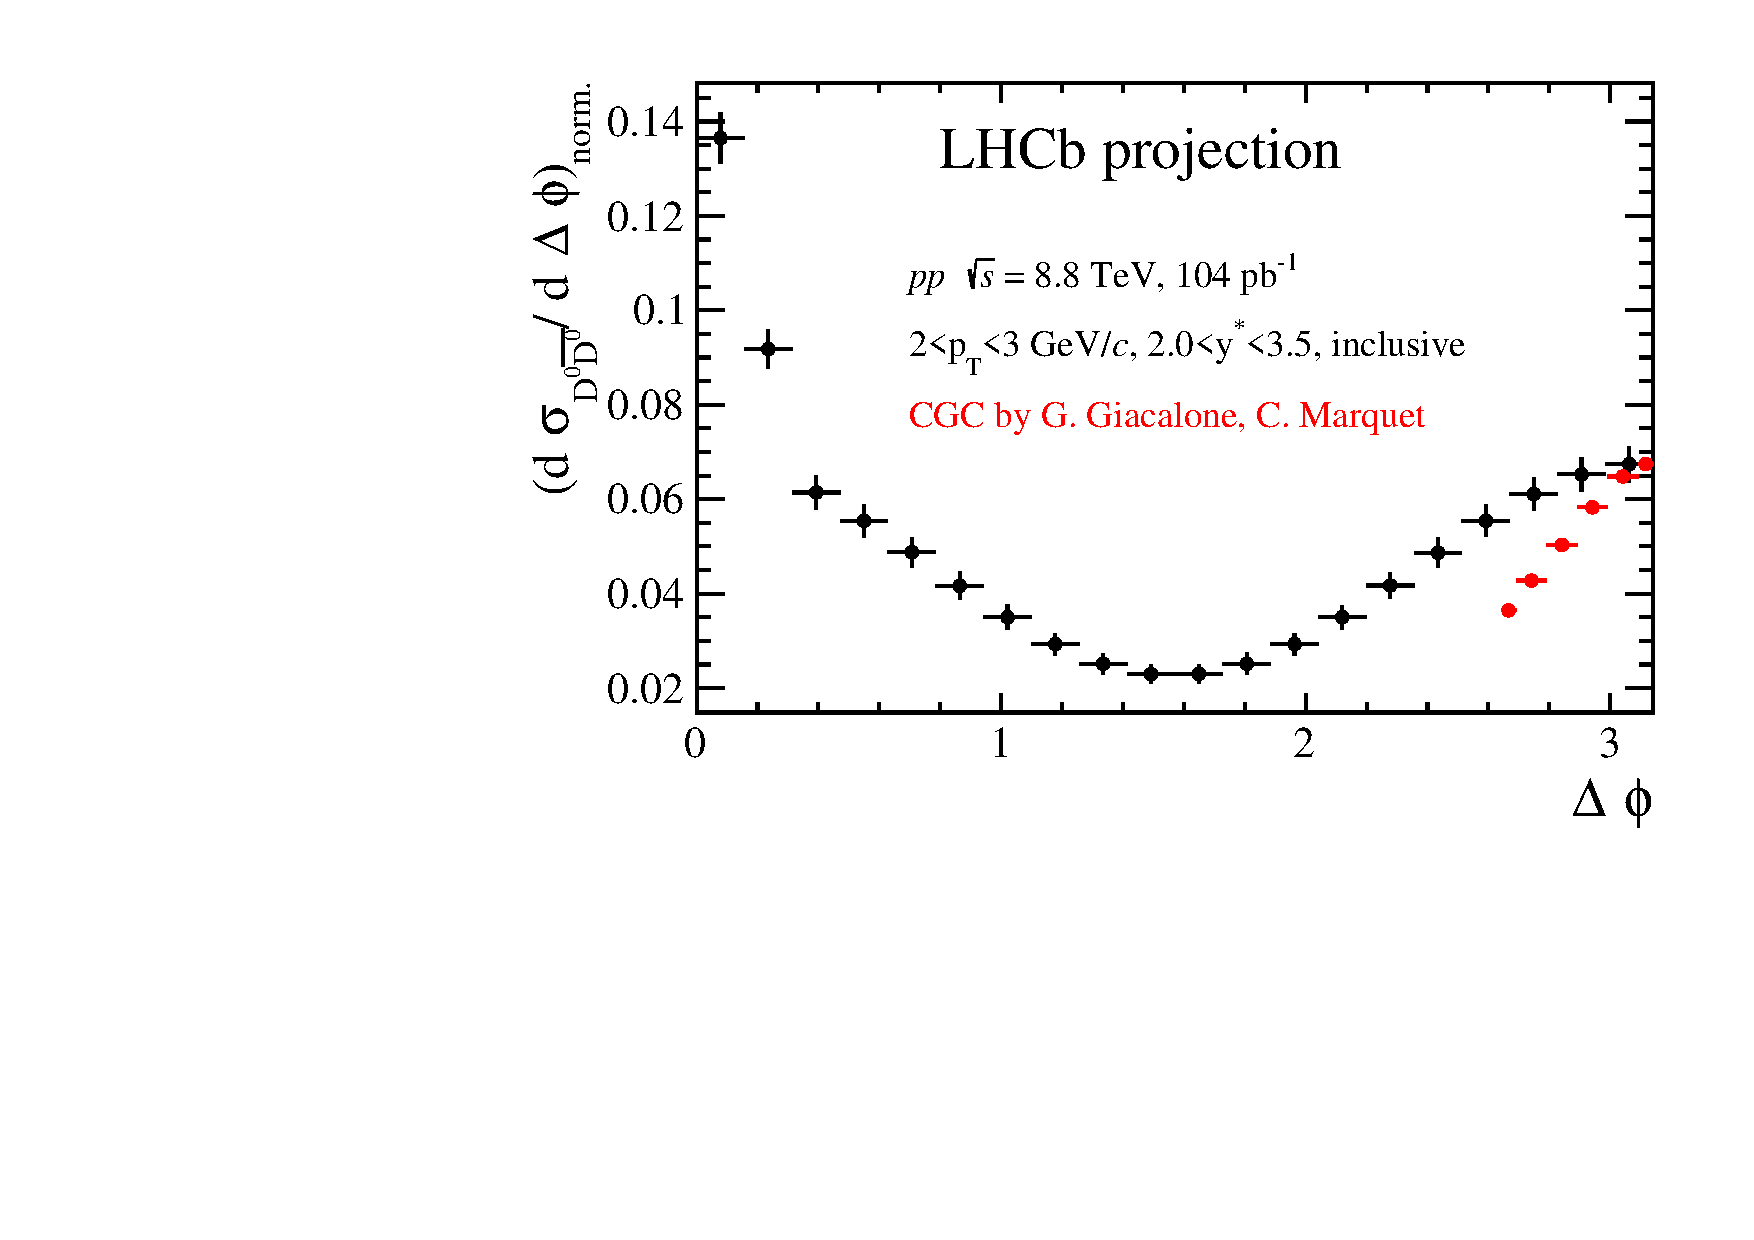
\includegraphics[width=.5\textwidth]{\main/smallx/fig/Deltaphi_overlappp.pdf}
\caption{ placeholder arbitrary normalisation for theory: LHCb projections for $D^0 \overline{D^0}$ in LHC Run 3 and Run 4 compared with theoretical calculations described in the text. The D-mesons are  both reconstructed in the piK-decay channel.}
\label{fig:ccbarlhcb}
\end{figure}

\subsubsection{Transverse momentum dependent and low-$x$ phenomena sensitive observables in $c\bar{c}$ and $b\bar{b}$ production }
%Editor:  Cyrille Marquet\\
%Content: c-cbar and b-bbar correlations: heavy-mesons and dijets \\
%Indicative length: 1-2 page

In recent years, many efforts have been devoted to elucidate the properties of transverse-momentum-dependent gluon distributions in the high-energy or small-$x$ limit, and in particular to determine how non-linear saturation effects impact the various distributions. A process which is particularly interesting in this regard is the forward production of a heavy quark-antiquark pair, in high-energy proton-proton or proton-nucleus collisions. For kinematical reasons, in such a process, the proton side of the collision involves large-$x$ partons, while on the nucleus side, small-$x$ gluons participate. Hence, this process can be described in a hybrid approach in which the proton content is described by regular, integrated PDFs, while the small-$x$ dynamics in the nuclear wave function is dealt with using the Color Glass Condensate (CGC) effective theory, from which the gluon TMDs naturally emerge \cite{Dominguez:2011wm,Marquet:2016cgx}.

In terms of sensitivity to the QCD saturation regime, the same manifestations are expected than with with light quarks \cite{Albacete:2018ruq}, although smaller values of x can be reached in the latter case. From the point of view of the TMD content however, heavy quarks are interesting because their production involves linearly-polarized gluons TMDs \cite{Akcakaya:2012si}, in addition to the usual unpolarized gluon TMDs, and because, due to non-linear effects, the linearly-polarized TMDs generally differ from their unpolarized partners \cite{Marquet:2017xwy}. The LHCb detector is well-suited to measure heavy hadrons in the forward rapidity region, and given large-enough statistics, one could potentially try and extract information about the linearly-polarized gluons in protons and lead nuclei, from data obtained the LHC unpolarized beams. Before we giving cross-section estimates, let us briefly give a bit more details about the process and the physics involved.

Forward quark-antiquark pair production in dilute-dense collisions is characterized by three momentum scales: $P_{t}$, the typical transverse
momentum of a single quark, and always one of the largest scales; $k_{t}$, the total transverse momentum of the pair, which is a measure of the transverse momentum of the small-$x$ gluons coming from the target; and $Q_s$, the saturation scale of the target, which is always one of the softest scales.
The value of $k_{t}$ with respect to $Q_{s}$ and $P_{t}$ governs which factorization scheme is relevant. Indeed, when $k_{t}\sim Q_{s}\ll P_{t}$ (the quark and the antiquark are almost back-to-back), there are effectively two strongly ordered scales $k_{t}$ and $P_{t}$ in the problem and TMD factorization applies \cite{Dominguez:2011wm}, implying the involvement of several gluon TMDs that differ significantly from each other, especially in the saturation regime, when $k_t\leq Q_s$ \cite{Marquet:2016cgx}. In the other regime which we shall not discuss here (away from back-to-back production), $k_{t}$ and $P_{t}$ are of the same order and far above the saturation scale, only the linear small-$x$ dynamics is important and the various TMDs differ no more.

In \cite{Marquet:2007vb,Dominguez:2011wm}, the cross section for forward di-jet production in proton-nucleus collisions
was calculated within the CGC. It was then shown that, in the back-to-back limit, a TMD factorization formula could
be extracted, the result being the same as in a direct TMD approach (i.e., without resorting to the CGC). However, in contrast to the
direct TMD approach, the calculation in the CGC yields explicit expressions for the TMDs in terms of Wilson lines, which can be evolved in rapidity
through the nonlinear Jalilian-Marian-Iancu-McLerran-Weigert-Leonidov-Kovner (JIMWLK) equation. In \cite{Marquet:2017xwy}, those results
were extended to the case of a forward heavy quark-antiquark pair. As already observed earlier (see for instance \cite{Mulders:2000sh,Boer:2009nc,Boer:2010zf,Metz:2011wb,dominguez:2011br,Akcakaya:2012si}), by keeping a non-zero quark mass, the cross section becomes sensitive to additional TMDs, which describe the linearly-polarized gluon content of the unpolarized target.

The three unpolarized gluon TMDs which describe the quark-antiquark pair production are the adjoint-dipole TMD, the Weizs{\"a}cker-Williams TMD, and a third one which is roughly a convolution of two fundamental-dipole TMDs. They are accompanied by three \textquoteleft polarized' partners, which couple through the quark mass and via azimuthal-angle modulation. This is analogous to what happens in the $\gamma^*A\rightarrow q\bar{q}$ process (in that case not only a non-zero quark mass but also a non-zero photon virtuality brings sensitivity to linearly-polarized gluons) described in Section~\ref{sec:upchqdijets},\ref{sec:upcdijets}, although there only one unpolarized gluon TMDs is involved (the Weizs{\"a}cker-Williams distribution), along with its polarized partner \cite{Metz:2011wb,dominguez:2011br}. %[Maybe refer to the photo production of dijets and heavy quarks sections ?]. MW: I simply put them now

Predictions for D mesons are presented in Figure \ref{fig:ccbarlhcb} as a function of their relative azimuthal angle near $\pi$, along with projections from the LHCb experiment. In the $p$Pb kinematical range that is investigated here, roughly 2.800~raw counts are expected over the full azimuthal range for the specified decay channel that can be complemented with other channels as in $pp$~collisions in Ref.~\cite{Aaij:2012dz}. %[Should we quote an expected number of events, in p+p and p+Pb, given the luminosities indicated ? That will depend on the decay channels used]




\subsubsection{Fully coherent energy loss effects on different final states}
\label{subsubsec:coherent}
%Editor: Francois Arleo\\
%Content: Drell-Yan/photons, E-loss, pt-broadening in pA\\
%Indicative length: 1-2 page

The multiple scattering of quarks and gluons traveling in a QCD medium induces the radiation of gluons which carry away some energy of the propagating parton, leading for instance to the jet quenching phenomenon. Therefore, a key ingredient of any parton energy loss calculation is  the medium-induced gluon spectrum radiated by the fast propagating color charge. It is of course of crucial importance to know the correct parametric dependence of the induced spectrum, which in general depends on the parton properties (in particular its energy and mass) and those of the medium, since it has a direct impact on the phenomenology of particle production in pA and AA collisions. The emission of a gluon radiated by an energetic parton experiencing multiple scattering in a medium takes a typical formation time, $t_f$, which needs to be compared to the length of the medium, $L$.

Over the last few years, it has been realized that in a hard process involving incoming and outgoing energetic color charges (which do not have to be identical) being quasi-collinear in the rest frame of the medium, the associated medium-induced gluon spectrum is dominated by {\it large} gluon formation times, $t_f \gg L$~~\cite{Arleo:2010rb,Peigne:2014rka,Peigne:2014uha}. In this so-called fully coherent (FC) region, the medium-induced radiated energy is similar to the energy loss of an asymptotic charge. In particular it scales as the energy, and thus exceeds at high energy the average parton energy loss in the Landau--Pomeranchuk--Migdal (LPM) regime, $t_f \lesssim L$, for which the energy dependence is at most logarithmic.
%
This different parametric behavior has important consequences on the phenomenology of hadron production in pA collisions. In particular, a model based on the fully coherent induced gluon spectrum was shown to describe accurately the quarkonium suppression observed in pA collisions at all center-of-mass energies, from the SPS fixed-target experiments ($\sqrt{s}\simeq 20$~GeV) to the LHC ($\sqrt{s}=5.02$~TeV and $\sqrt{s}=8.16$~TeV)~\cite{Arleo:2012hn,Arleo:2012rs,Arleo:2013zua}. It is therefore necessary to investigate further the role of fully coherent energy loss on other processes.
%
Because the fully coherent induced gluon spectrum arises from the interference between the emission amplitudes off the initial charge and that off the final state, the effects of FC energy loss are process dependent. Let us review, at a qualitative level, the expected nuclear dependence of different processes which could be measured at the LHC with a high luminosity.

In the absence of color charge in the partonic final state, the energy loss in Drell-Yan (DY) production at leading order is expected to be that of a suddenly decelerated parton, that is, independent of its energy (LPM regime). The effects of parton energy loss in nuclei should therefore play almost no role on DY production in high-energy pA collisions, since $\Delta E / E \to 0$ in the high-energy limit. The inclusive production of DY lepton pairs in pA collisions at the LHC should therefore be free of any parton energy loss effect. As a result, this process might be used advantageously in order to probe possible nuclear PDF effects at small values of $x$, see \eg Fig.~\ref{fig:plotDY} and Ref.~\cite{Arleo:2015qiv} for more details. Assuming a luminosity of ${\cal L}=250$~nb$^{-1}$ and taking the conservative value for the cross section in pPb collisions at $\sqrt{s}=5$~TeV, ${\rm d}\sigma/dy=40$~nb~\cite{Arleo:2015qiv}, the number of forward DY lepton pair, which could be measured by the LHCb experiment is typically $10^4$ per rapidity unit. Also interesting, and accessible with a high luminosity, would be the production of diphotons in pA collisions. This process would be free of energy loss effects, for the same reasons as the DY process, while being sensitive to nPDF in the quark sector, $q\bar{q} \to \gamma\gamma$, and in the gluon sector through the `box diagram', $gg \to \gamma\gamma$.

Note that the energy loss scaling as $E$ (FC regime) would come into play only if {\it another} energetic charged particle is produced in the final-state in association with the virtual photon (or the diphoton), such that the final state carries a global color charge. Such a situation typically occurs in DY$+$jet production in pA collisions. Consider for instance the Compton scattering process, $qg \to q\gamma^\star$. At forward rapidity, an incoming quark from the proton projectile scatters in the medium to produce the final state in a color triplet representation. In this peculiar case of quark to a color triplet final state, one would expect a negative medium-induced gluon spectrum, leading to an energy \emph{gain} (with respect to pp collisions), $\Delta E \propto (-1/2N_c)\times E$. Such an unusual dependence would manifest by a slight \emph{enhancement} of DY+jet production in pA collisions with respect to pp collisions, although a quantitative study would be needed to answer whether this effect could be visible in the experiment. Similarly, should this enhancement be small or negligible, the associate production of a prompt photon with a heavy-quark jet might be sensitive to the nPDF of heavy quarks and gluons, as emphasized in Ref.~\cite{Stavreva:2010mw}. Using $\sigma_{\gamma c} = 1.2\times10^5$~pb in the acceptance of the ALICE calorimeter~\cite{Stavreva:2010mw} leads to $2.4\times10^5$ $\gamma+c$-jet events in pPb collisions at $\sqrt{s}=8.8$~TeV assuming ${\cal L}=2$~pb$^{-1}$.

More pronounced effects of fully coherent energy loss are expected when the final state is in a color octet state, or possibly in higher color representations. An example is the production of a jet pair with not too large transverse momenta (ideally only a few times the saturation scale of the target nucleus). In the case of di-gluon production, the final state can be produced in the 27-plet color representation (with Casimir $C_{27}=8$) that would lead to an average coherent energy loss proportional to $(N_c+C_{27})/2=11/2$, that is almost twice larger that expected if the final state is in a color octet state. Such higher color representations could also be probed in the production of $B_c$ mesons (or in the associate production of a D and a B meson), with a complex final state $c\,\bar{c}\,b\,\bar{b}$. From the number of fitted signal candidates ${\cal N}=10^4$ $B_c$ mesons extracted at LHCb in the semileptonic decay channel in pp collisions at $\sqrt{s}=8$~TeV with ${\cal L}=2$~fb$^{-1}$~\cite{Aaij:2014bva}, the expected $B_c$ rate in the LHCb acceptance using ${\cal L}=0.5$~pb$^{-1}$ in pPb collisions at the same energy is ${\cal N}=5\times 10^2$ $B_c$ mesons.

%%%%%%%%%%%%%%%%%%%%%%%%%%%%%%%%%%%%%%%%%%%%%%%%%%%%%%%%%%%%%%%%%%%5
\subsection{Constraints on nuclear PDFs at the HL-LHC}
\label{sec:nPDFs}
%Editors: see subparts\\
%Indicative length: 5 pages
\subsubsection{Overview}
%Editors: Fred Olness, Aleksander Kusina, Ingo Schienbein, Hannu Paukkunen,   Ilkka Helenius\\
%Indicative length: 2 pages 
% 
% \color{blue}
% Content: summary of 'safe' inputs referring to sub-chapter tables, discussion of their impact and global fit to  pseudodata and discussion of theory progress to enlarge 'safe' observables: low-x resummation, NNLO for heavy-quark c,b observables, necessary input assumptions and how to confirm/falsify with measurements
% outlook trying to fold in progress to be expected from experiment/theory and also consequences for Initial state description in heavy-ions.  OUTLINE: sketch current status/uncertainty, short-comings (u/d asymmetry, strange),
% and where improvements can be expected.
% updates from cms\cite{Chatrchyan:2013uja} and atlas\cite{Aad:2014xca}
% \color{black}
%%%%%%%%%%%%%% END OF TEXT COLOR

% FRED NOTE: GIVE OUR SPACE CONSTRAINTS, WE WILL REFERENCE THE RESULT BUT NOT SHOW THE FIGURE
%
%  NNPDF Figure: Impact of nuclear data   
%%%%%%%%%%%%%%%%%%%%%%%%%%%%%%%%%%%%%%%
% \begin{figure}[tbh] %%%%%%%%%%%%%%%%%%%%%
% \centering{} 
% 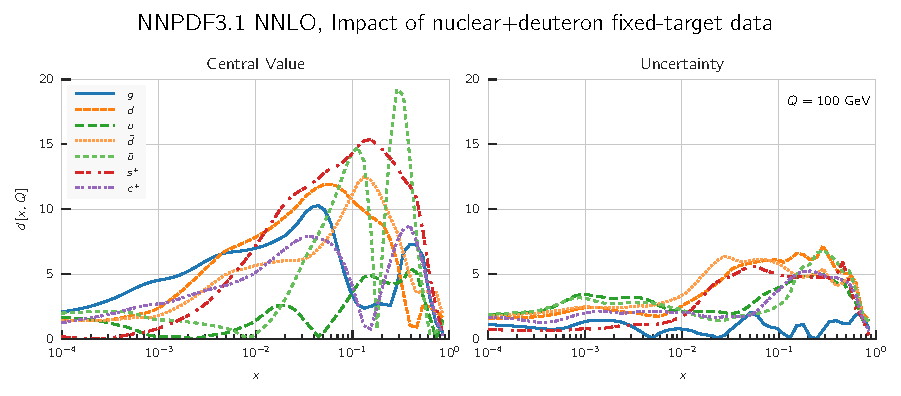
\includegraphics[width=0.85\textwidth]{\main/smallx/fig/distances_proton2.pdf}
% \caption{
% The impact of removing the nuclear data from the PDF fit  
% in terms of the distance measure $d[x,Q]$;  here,  $d \sim 10$ corresponds to a one sigma variation. 
% Figure from  Ref.~\cite{Ball:2017nwa}.
% }
% \label{fig:nnpdfDistance}
% \end{figure}
%%%%%%%%%%%%%%%%%%%%%%%%%%%%%%%%%%%%%%%%%%%%


As previously discussed in Sec.~\ref{sec:smallxIntro}, 
the nuclear Parton Distribution Functions (nPDFs) 
are poorly constrained as compared the the proton PDFs. 
This is mainly due to the lack of high statistics data 
across the very  large nuclear $A$-range. 
%
In fact, even the precision of the proton PDFs  rely crucially on 
nuclear target data~\cite{Ball:2017nwa,Dulat:2015mca,Alekhin:2017kpj};
for example,  the neutrino-nucleon DIS structure functions 
are essential for decomposing the flavor components of the 
proton~\cite{Onengut:2005kv,Goncharov:2001qe,Mason:2006qa,Samoylov:2013xoa,KayisTopaksu:2011mx}.
%
Consequently, improved determinations of the nuclear PDFs and nuclear correction factors 
could improve the proton PDF precision.
%
Thus, a HL-LHC could provide the opportunity to precisely determine 
the nPDFs across a large range of $A$ values, and thereby
disentangle the nuclear effects from the individual flavor components. 

%%% Ball:2017nwa,  NNDPF [arXiv:1706.00428]  uses 
%%% Onengut:2005kv,  CHORUS inclusive neutrino DIS [Phys. Lett. B632 (2006) 65–75], 
%%% Goncharov:2001qe,Mason:2006qa,  and NuTeV dimuon production data [hep-ex/0102049, FERMILAB-THESIS-2006-01]
%%% 
%%% Dulat:2015mca, CT14 [arXiv:1506.07443] uses  dimuon production in neutrino collisions from the 
%%% Goncharov:2001qe,  CCFR [hep-ex/0102049] and 
%%% Mason:2006qa,      NuTeV [ FERMILAB-THESIS-2006-01,UMI-32-11223] 
%%% 
%%% Alekhin:2017kpj,  ABMP16 [arXiv:1701.05838] uses charm-quark production in CC neutrino-nucleon DIS collected by the 
%%% Samoylov:2013xoa, NOMAD [ arXiv:1308.4750] and 
%%% KayisTopaksu:2011mx, CHORUS [arXiv:1107.0613] as well as 
%%% CCFR [hep-ex/0102049] and 
%%% Goncharov:2001qe,  NuTev [hep-ex/0102049] 
%%% 

\subsubsection{$W^\pm$/Z Production}
%Editors: Fred Olness, Aleksander Kusina, Ingo Schienbein.

%  ATLAS s(x) measurement;  
%%%%%%%%%%%%%%%%%%%%%%%%%%%%%%%%%%%%%%%
\begin{figure}[tbh] %%%%%%%%%%%%%%%%%%%%%
\centering{} 
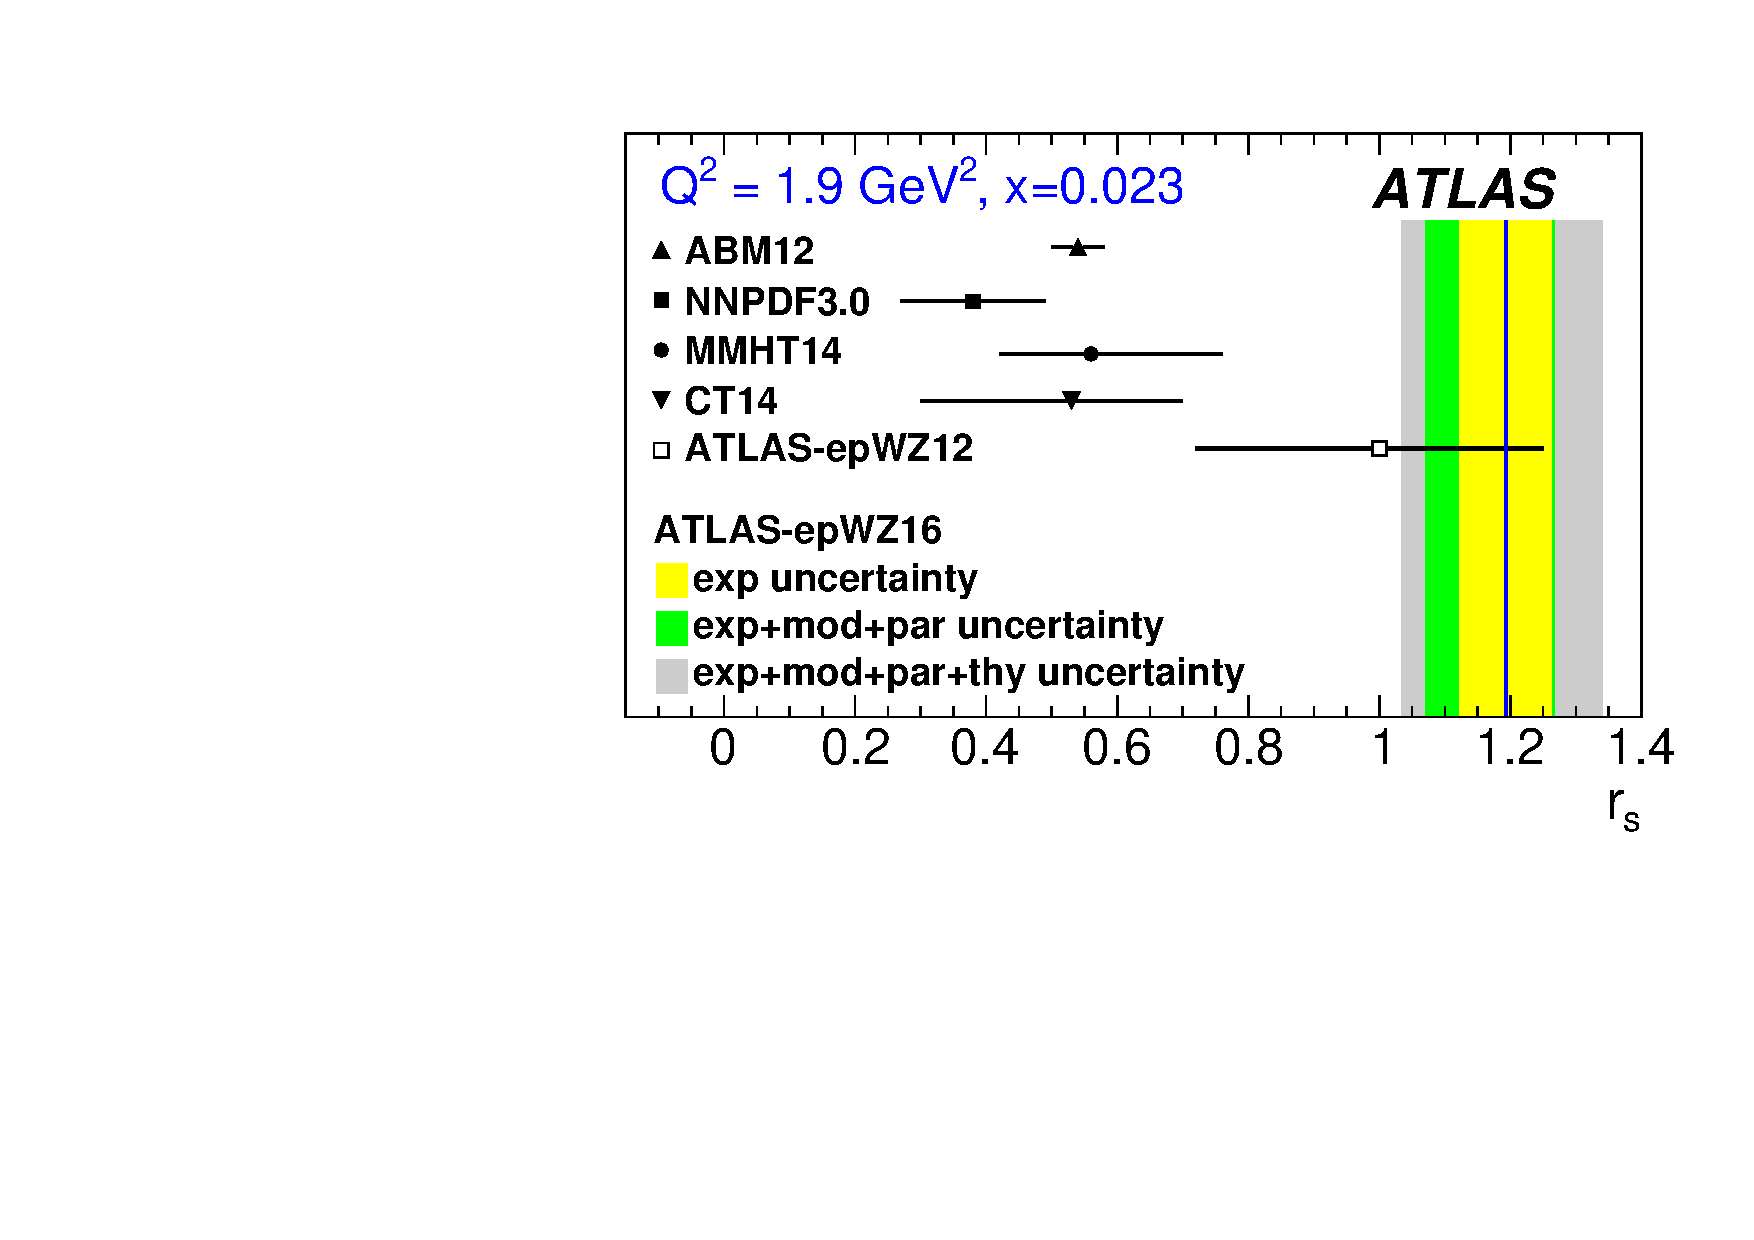
\includegraphics[width=0.30\textwidth,height=0.27\textwidth]{\main/smallx/fig/atlas_fig_31a.pdf}
\hfil
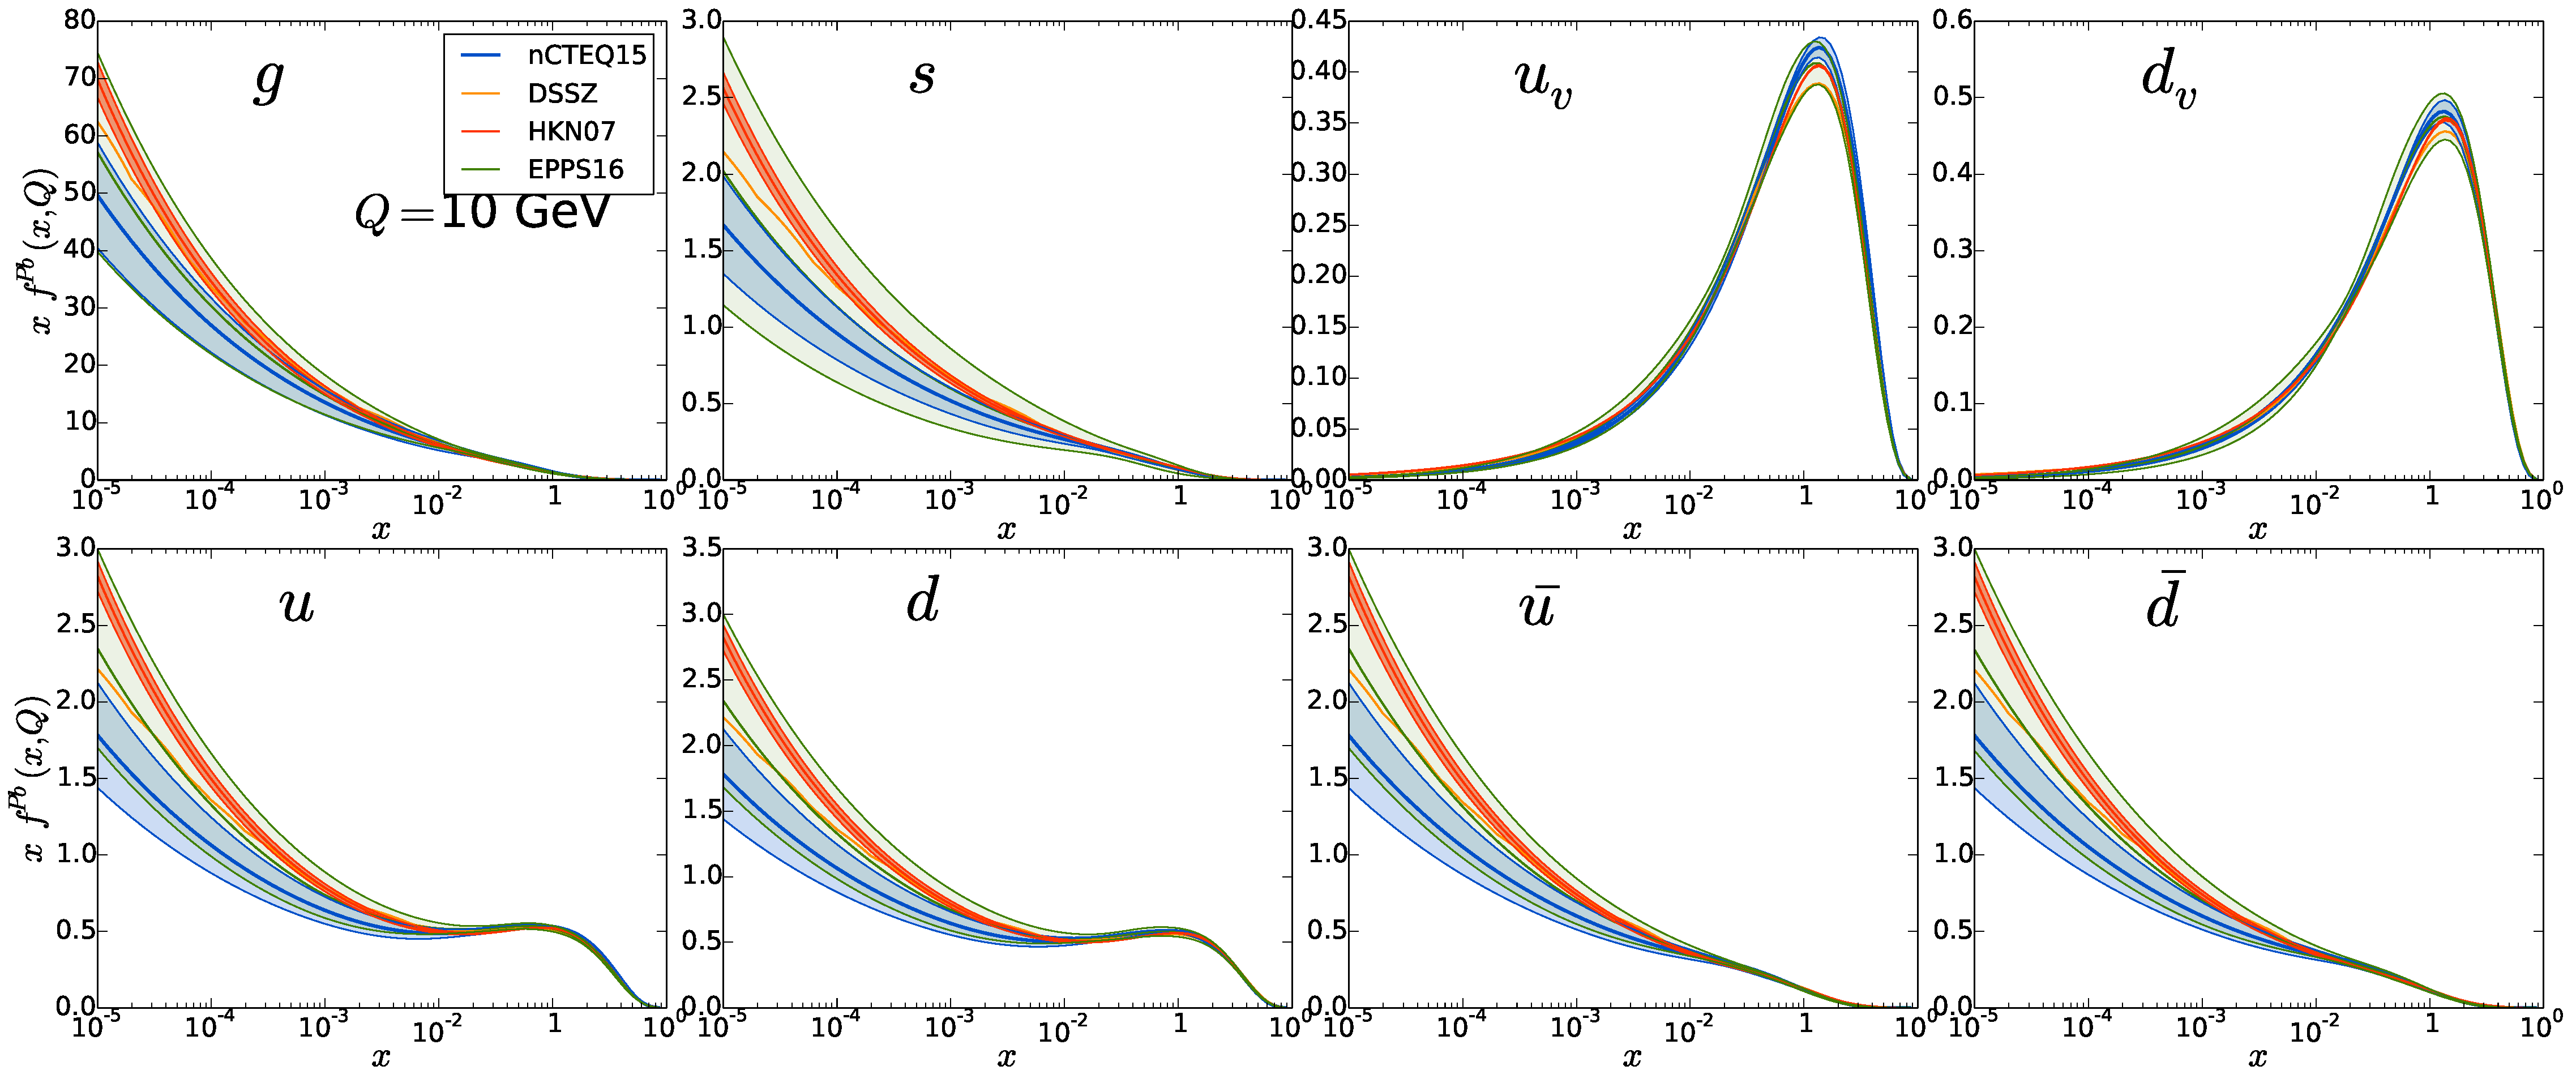
\includegraphics[trim=0cm 16.3cm 38.2cm 0cm, clip=true,width=0.68\textwidth]{\main/smallx/fig/nCTEQ-FullPDFs_Q10.pdf}
\caption{
a) Determination of the relative strange-to-down sea quark fractions 
$r_s=0.5(s + \bar{s})/\bar{d} $ as compared with  predictions from different NNLO PDF sets. Figure from Ref.~\cite{Aaboud:2016btc}.
Comparison of the b) gluon and c) strange quark nPDF for a lead nucleus as a function of $x$ for 
a selection of nuclear PDF sets:
HKN07~\cite{Hirai:2004wq}, DSSZ~\cite{deFlorian:2011fp}, EPPS16~\cite{Eskola:2016oht}, and nCTEQ15\cite{Kovarik:2015cma}.
}
\label{fig:atlas_s}
\label{fig:npdf}
\end{figure}
%%%%%%%%%%%%%%%%%%%%%%%%%%%%%%%%%%%%%%%%%%%%


%     WZ Cross section correlation  %%%  Lumonisty  figure
%%%%%%%%%%%%%%%%%%%%%%%%%%%%%%%%%%%%%%%
\begin{figure}[t] %%%%%%%%%%%%%%%%%%%%%
\centering{} 
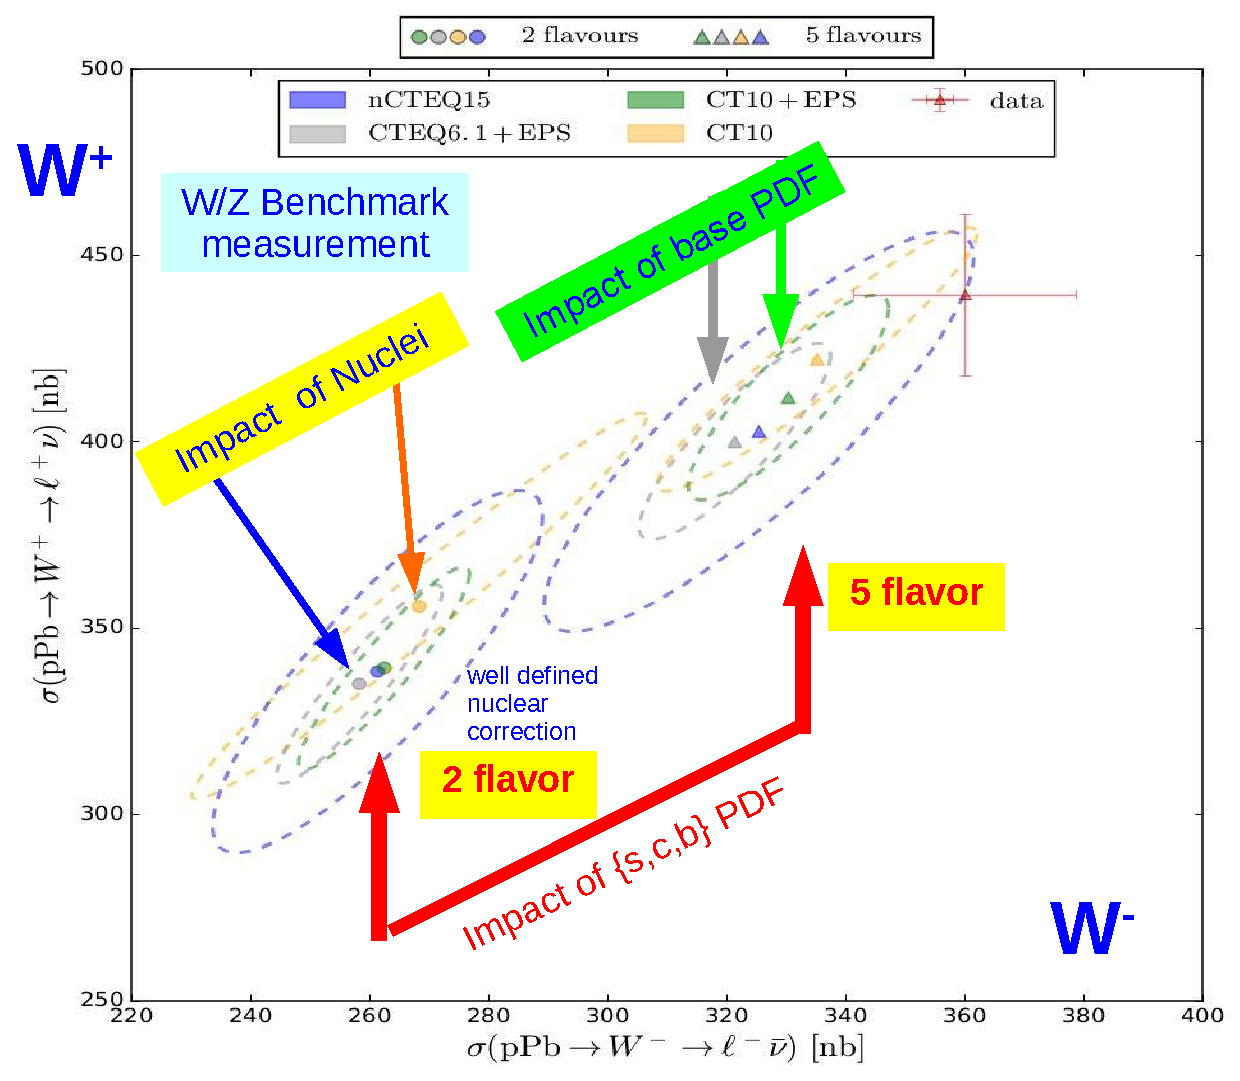
\includegraphics[width=0.48\textwidth,height=0.40\textwidth]{\main/smallx/fig/WZcorr_nuc.pdf}
\hfil
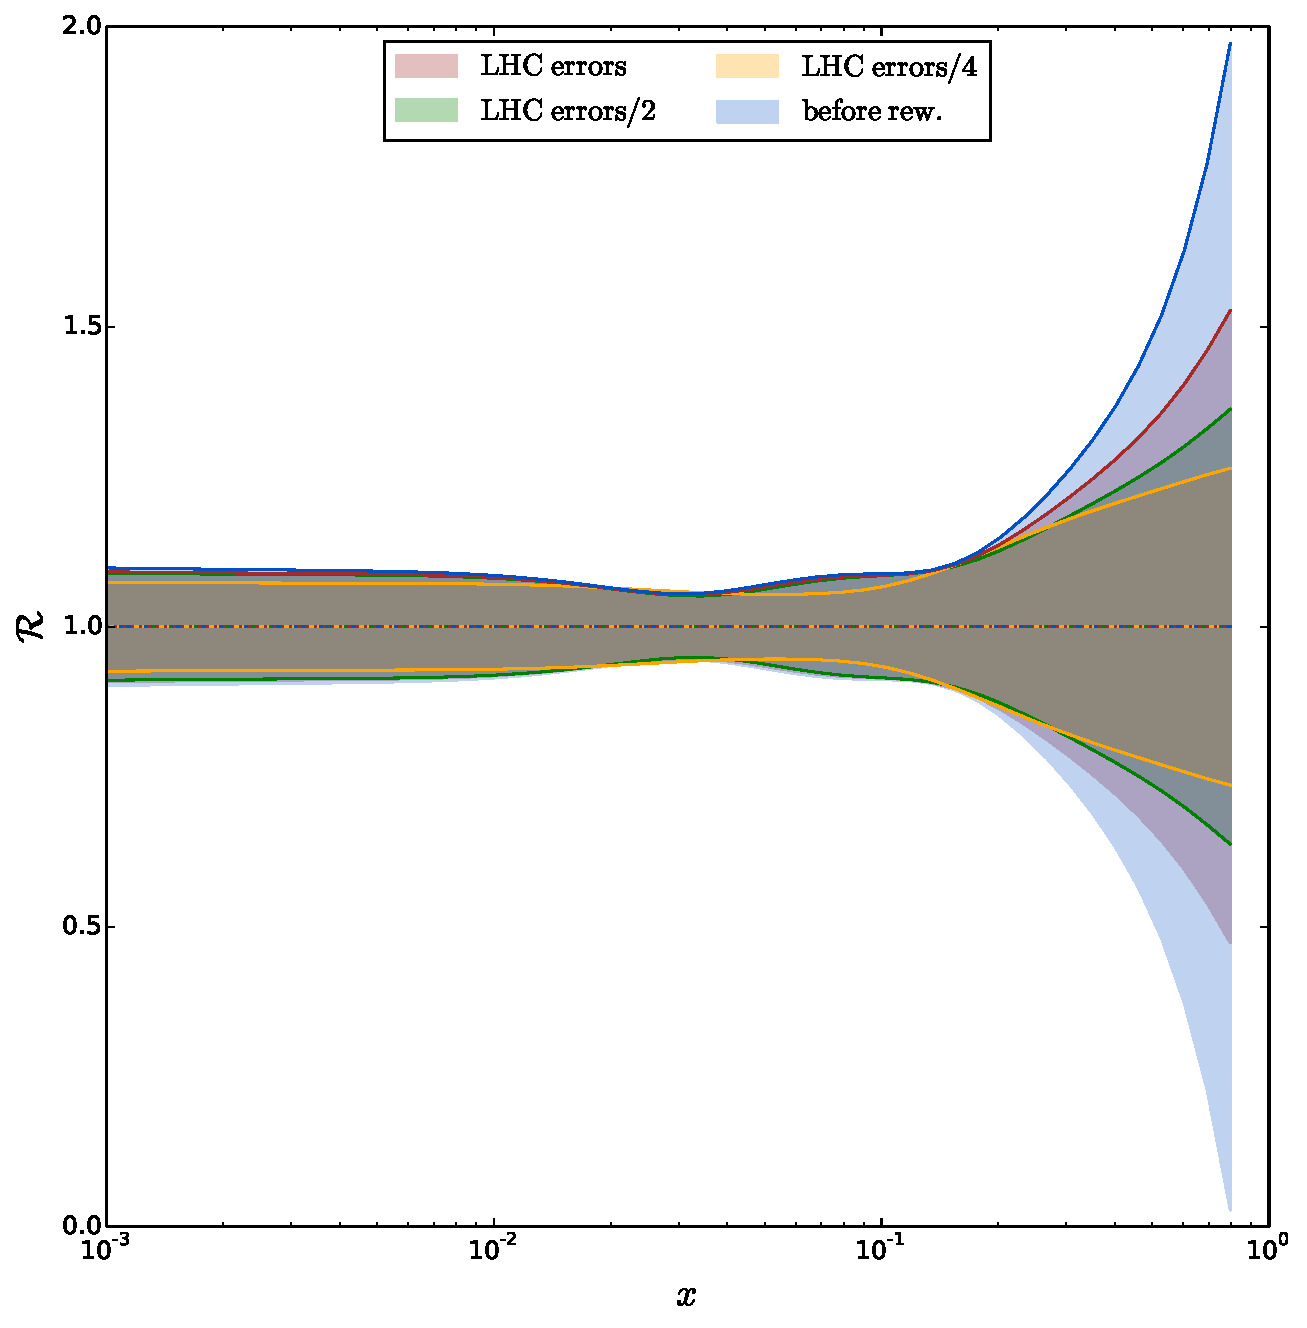
\includegraphics[width=0.45\textwidth,height=0.40\textwidth]{\main/smallx/fig/wlum}
\caption{
a)~Correlations between $W^+$ and $W^-$ cross sections calculated with different input PDFs and assumptions for the $pPb$ process to illustrate the separate impact of the 
i)~nuclear corrections, ii)~heavy flavor components, and iii)~base PDFs; 
figure based on Refs.~\cite{Kusina:2016fxy,Godat:2018kgp}.
\\\hspace{\textwidth}
b)~We display the PDF uncertainty of the gluon $g(x)$ at $Q=10$~GeV 
as a function of $x$. 
The outermost band (blue) is the nCTEQ15 PDFs with no LHC data. 
The next (red) band reweights the nCTEQ15 PDFs with the LHC $\sqrt{s}=5.02$~TeV $pPb$ data. 
The next two bands (green, yellow) illustrate the effect of reducing the experimental uncertainties 
by factors of 2 and 4, respectively.\label{fig:WZcorr}
}
\end{figure}
%%%%%%%%%%%%%%%%%%%%%%%%%%%%%%%%%%%%%%%%%%%%

% Hannu & Ilkka, thanks for the comments. Let me know if the revised takes care of this. Fred


%%%%%%%%%%%%%%%%%%%%%%%%%%%%%%%%%%%%%%%%%%%%%%%%%%%%%%%%%%%%%%%%%%%
\noindent {\bf $W/Z$ Inclusive Production:}
%
%%%  Aad:2015gta, ATALS Z [arXiv:1507.06232]
%%%  TheATLAScollaboration:2015lnm,  ATALS W [http://cds.cern.ch/record/2055677]
%%%  Khachatryan:2015pzs, CMS Z [arXiv:1512.06461]
%%%  Khachatryan:2015hha, CMS W [arXiv:1503.05825; ]
%%%  CMS:2018ilq,[http://cms-results.web.cern.ch/cms-results/public-results/preliminary-results/HIN-17-007/index.html]
%%%  Aaij:2014pvu, LHCb Z [arXiv:1406.2885]
%%%  Alice:2016wka, ALICE W,Z [arXiv:1611.03002]
%
Inclusive production of $W/Z$ bosons in $pp$ collisions at the LHC  can provide
new information on the $\{s,c,b\}$ PDFs.
% DISCUSS LATER: as well as associate production channels such as $Wc$ and $Wb$. 
Additionally, heavy ion $W/Z$ production data from $pPb$ and $PbPb$ can provide insight on 
the nuclear corrections, 
and this complements other data on nuclear targets as it is at large $A$ (lead) and high energy (and thus, smaller $x$)~\cite{Aad:2015gta,TheATLAScollaboration:2015lnm,Khachatryan:2015pzs,Khachatryan:2015hha,CMS:2018ilq,Aaij:2014pvu,Alice:2016wka}.
%
%
For example, ATLAS used  inclusive $W/Z$ production data to extract the strange component of the proton; 
as displayed in Fig.~\ref{fig:atlas_s}  this yielded a larger strange PDF than commonly expected~\cite{Aad:2012sb,Aaboud:2016btc}. 
%
A recent analysis of the ATLAS and CMS inclusive W and Z differential
cross-section data at 7 and 8 TeV~\cite{Cooper-Sarkar:2018ufj}
(including the combined HERA inclusive data) indicates that while there is no tension between the
data sets, the  LHC data does support unsuppressed strangeness
in the proton at low x at both low and high scales. 
Certainly this is an area that warrants further study. 

To highlight the sensitivity of the heavy ion $W/Z$ production to both the 
heavy flavor components and the nuclear corrections, 
in Fig.~\ref{fig:WZcorr} we display the correlations between $W^+$ and $W^-$ 
cross sections for proton-lead interactions calculated with different input PDFs and assumptions~\cite{Kusina:2016fxy}.
%
By comparing the results with and without the $\{s,c,b\}$ flavors, we see these quarks do have a
large impact on this observable;  hence, this process can provide incisive information about the 
corresponding PDFs. 
%
To see the effect of the nuclear corrections, we can compare the CT10 proton result with the other calculations. 
%
We observe that for the case of 2 flavors only, the separation of the proton result  (CT10) and the 
nuclear results are quite distinct. In this case, the effect of the specific nuclear correction (nCTEQ15 or EPS09)
or the effect of the underling base PDF (CTEQ6.1 or CT10) is minimal. 
%
In contrast, when we compare this picture to the 5 flavor results, the division between the proton and nuclear
result is not as simple as the different nuclear corrections and base PDFs yield a broader range of results. 
In particular, we note that the strange quark PDFs in the CTEQ6.1 and CT10 base PDFs are quite different, and this will contribute to the spread of results. 
%
Thus, proton-lead  production of $W/Z$  is an ideal ``laboratory'' 
as this process is sensitive to i)~the heavy flavor components,
ii)~the nuclear corrections, and iii)~the underlying ``base'' PDF. 

To illustrate the potential improved nPDF constraints from the W/Z data, 
in Fig.~\ref{fig:WZcorr}-(b) we display the PDF uncertainty for the gluon.
The bands show the results without LHC data (the original nCTEQ15 result in blue), 
then including the  LHC $\sqrt{s}=5.02$~TeV $pPb$ data, 
and finally a assumed reduction of the experimental errors by a factor of 2 and 4.
%
Thus, a dedicated high-statistics heavy  ion run at a HL-LHC has the potential 
to reduce  the current uncertainties and improve the nuclear PDF determiniation, 
especially in the high $x$ region. 


%%%%%%%%%%%%%%%%%%%%%%%%%%%%%%%%%%%%%%%%%%%%%%%%%%%%%%%%%%%%%%%%%%%
% Hannu, thanks for this discussion. I've now integrated this into the section. 
% Please edit as you like. Fred
% P.S. We looked at the asymmetry with the 5.02TeV data, but much of the nuclear effects 
% dropped out in the ratio. Maybe if we had HL this would not be an issue?

% I believe the principal issue is that the 5TeV data is binned in lab-frame rapidity variable - not the rapidity in the center-of-mass frame.  Hannu 


%%%%%%%%%%%%%%%%%%%%%%%%%%%%%%%%%%%%%%%%%%%%%%%%%%%%%%%%%%%%%%%%%%%
\noindent {\bf W Asymmetry Ratios:}
%
A complementary method  to disentangle the nuclear effects
from proton PDF and other theory uncertainties like higher-order
effects is to form the nuclear modification factor 
$R_{{\rm p}A} = \sigma^{{\rm p}A}/\sigma^{{\rm p}{\rm p}}$.
Although the on-shell W$^\pm$ production probes the PDFs in a rather
narrow $x$ window, the W$^\pm$ case is complicated by the significant
isospin effect for which $R_{{\rm p}A} \neq 1$ even in the absence of
nuclear effects in PDFs. This partly undermines the clear extraction
of the nuclear PDFs. To overcome this difficulty the asymmetry
$(\sigma^{W^+(y^*)}-\sigma^{W^+(-y^*)})/(\sigma^{W^-(y^*)}-\sigma^{W^-(-y^*)})$
has been proposed \cite{Paukkunen:2010qg} as an alternative. In order to measure such a quantity involving four cross sections and subtractions among them (particularly in the denominator which may go close to zero), a good statistical precision --- like that achievable at the HL-LHC would be advantageous.

%%%%%%%%%%%%%%%%%%%%%%%%%%%%%%%%%%%%%%%%%%%%%%%%%%%%%%%%%%%%%%%%%%%
%
\begin{figure}[htb!]
\centering
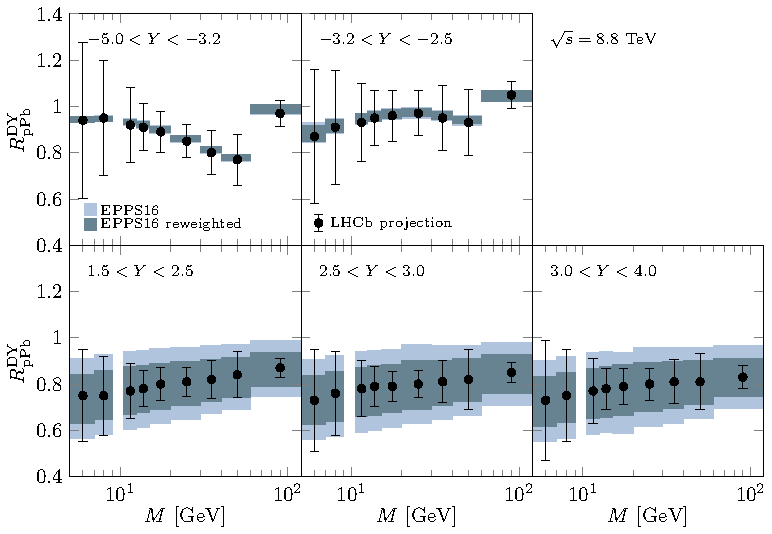
\includegraphics[width=0.565\textwidth]{\main/smallx/fig/HLLHC_DY.pdf}
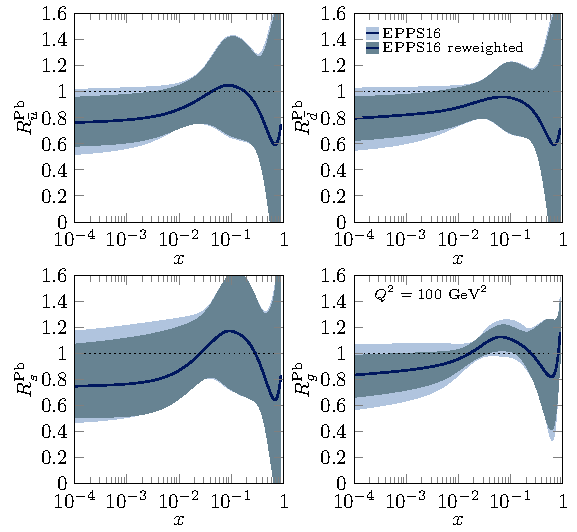
\includegraphics[width=0.425\textwidth]{\main/smallx/fig/HLLHC_nPDFs_100_GeV2.pdf}
\caption{Left: The LHCb projections on $R_{\rm pPb}$ in  Drell-Yan process compared to the original EPPS16 error bands and those after reweighting with these data. Right: The improvement in EPPS16 nuclear PDFs for sea quarks and gluons at $Q^2=100\,{\rm GeV^2}$ upon reweighting with the data shown in the left-hand panel.}
\label{fig:DYRpPb}
\end{figure}

\noindent {\bf Low-mass Drell-Yan:}
%
In the case of on-shell Z production, the isospin effect is much milder \cite{Paukkunen:2010qg} and poses less difficulties. This advantage is partly lost at low invariant mass (Drell-Yan region) which, however, is precisely the luminosity-hungry zone where the HL-LHC can make a difference. It would be very much advantageous to reach this low-mass region experimentally as it offers a possibility to constrain the nuclear PDFs at lower factorization scale where the nuclear effects are larger. The estimated impact is shown in Fig.~\ref{fig:DYRpPb} where the LHCb estimates for $R_{\rm pPb}$ are compared to the reduction of EPPS16 uncertainties upon performing a PDF reweighting \cite{Paukkunen:2014zia} with these data. Although the Drell-Yan process occurs predominantly via $q\overline{q}$ annihilation, the scale-evolution effects are large and these data mostly constrain the gluon PDFs. Here, it should be noted that here the probed $x$ values are already so small, that the parametrisation bias which is prominen at small $x$ \cite{Aschenauer:2017oxs, Paukkunen:2017phq} is probably significant and understates the "true" effect of these measurements. This kind of scan over a wide range of invariant masses with HL-LHC precision would offer a possibility to test the $Q^2$ evolution of nuclear PDFs -- whether there are corrections to standard DGLAP -- much more systematically than only on-shell W$^\pm$- and Z-production measurements do.

%Precise measurements on Drell-Yan and W$^\pm$ have also potential to be useful for free proton PDFs: Indeed, if the information on nuclear effects are first extracted via ratio observables which are not too sensitive to the proton PDFs, the absolute spectra can subsequently be fed in the free proton analysis. The point is that p-$A$ collisions are sensitive to different linear combinations of partons than in the p-p case --- this is exactly the reason why e.g. deeply inelastic data on Deuteron are still being used in free proton fits despite the complications of nuclear corrections. 



%%%%%%%%%%%%%%%%%%%%%%%%%%%%%%%%%%%%%%%%%%%%%%%%%%%%%%%%%%%%%%%%%%%
% MOVED TO THE HEAVY QUARK SECTION:
%\noindent {\bf $WQ$ Associated Production:}
%

%%%%%%%%%%%%%%%%%%%%%%%%%%%%%%%%%%%%%%%%%%%%%%%%%%%%%%%%%%%%%%%%%
\subsubsection{Dijet Production}

%Editors: Hannu Paukkunen ... \\
%Indicative length: 1-2 pages 

\textcolor{blue}{HP as of 13.9: Yen-Jie's group still working on enlarging the kinematics. We are waiting for their input. The profit of HL-LHC over Run II data probably at high $p_{\rm T}$ \& large/small rapidity.}

% \noindent
% \textcolor{blue}{note: as nCTEQ does not yet have this implemented,
% will need to extrapolate from EPPS16\cite{Eskola:2016oht} for this assessment.}
% \\
% We suggest (Fred \& Ingo) keeping this separate from UPC 
% to keep the $hh$ separate from the effective $h \gamma$ 
% (the $\gamma$ includes both direct and resolved contributions) as well as other issues.



%%%%%%%%%%%%%%%%%%%%%%%%%%%%%%%%%%%%%%%%%%%%%%%%%%%%%%%%%%%%%%%%%%%%%%%%%%%
\subsubsection{Heavy Quark Production}
%Editors: Ingo Schienbein, Aleksander Kusina, Fred Olness ... \\
%Indicative length: 1-2 pages 


%%%%%%%%%%%%%%
\noindent\textbf{Inclusive Heavy Quark Production:} 
%
A recent study of  inclusive heavy quark
production in proton--lead collisions at the LHC 
demonstrates this can also help constrain  the gluon distribution in nuclei.
%
Specifically, Ref.~:\cite{Kusina:2018pbp} makes use  of LHC $pPb$ data on 
$\{D^0, J/\Psi, B\to J/\Psi, \Upsilon(1S)  \}$ meson production~\cite{Abelev:2014hha,Adam:2016ich,Aaij:2017gcy,Adam:2015iga,Aaboud:2017cif,Abelev:2013yxa,Aaij:2013zxa,Aaij:2017cqq,LHCb:2018jln,Abelev:2014oea,TheATLAScollaboration:2015zdl,Aaij:2014mza}.
%
They obtain a consistent description of these data assuming nPDF
modifications are the dominant source of nuclear modifications in $p-Pb$
collisions. Under this assumption, a clear confirmation of gluon
shadowing at small-$x$ is found.  Additionally, they demonstrate that
the inclusion of such heavy-flavour data in a global fit can
significantly reduce the uncertainty on the gluon density down to
$x\simeq 7 \times 10^{-6}$ while keeping an agreement with the other
data of the global fits.  A reweighting of the current nPDFs sets with
the LHC heavy-flavour data was performed for the nCTEQ15 and EPPS16
sets.  In a recent analysis of beauty hadrons by the LHCb
collaboration~\cite{Aaij:2013zxa,Aaij:2017cqq,LHCb:2018jln} excellent agreement between the reweighted
predictions and the measured data for the nuclear modification factor
$R_{pPb}$ was found. Furthermore, the precision of these data will
allow to further reduce the uncertainty of the low-$x$ nuclear gluon
distribution. Due to the lower production rates for beauty hadrons,
this kind of observables would clearly profit from a higher
luminosity.  Note that heavy flavour measurements from LHCb extending
to larger transverse momenta have also the potential to constrain the
intrinsic heavy quark component~\cite{Kniehl:2009ar,Brodsky:2015fna,Lyonnet:2015dca}.
%
%\cite{0901.4130,1504.06287,1504.05156}.
%%%  Abelev:2014hha,Adam:2016ich,   ALICE D0 [arXiv:1405.3452; arXiv:1605.07569]
%%%  Aaij:2017gcy, LHCb D0 [arXiv:1707.02750]
%%%  Adam:2015iga, ALICE J/psi [arXiv:1503.07179]
%%%  Aaboud:2017cif, ATLAS J/psi [arXiv:1709.03089]
%%%  Abelev:2013yxa,  LHCb J/psi [arXiv:1308.6726]
%%%  Aaij:2013zxa,Aaij:2017cqq, LHCb B->J/psi [arXiv:1308.6729; arXiv:1706.07122]
%%%  LHCb:2018jln,  LHCb B+ [https://cds.cern.ch/record/2641671/files/LHCb-CONF-2018-004.pdf]
%%%  Abelev:2014oea,  ALICE Upsilon(1S) [arXiv:1410.2234]
%%%  TheATLAScollaboration:2015zdl,  ATLAS Upsilon(1S) [ATLAS-CONF-2015-050]
%%%  Aaij:2014mza,   LHCb Upsilon(1S) [arXiv:1405.5152]
%%%  



%%%%%%%%%%%%%%
\noindent\textbf{Prompt Photon-Production and Diphoton Production } 
%
As discussed in Sec.~\ref{subsubsec:coherent}, other nuclear effects such
as coherent small angle gluon radiation may explain the heavy-flavour
data without a strong shadowing of the small-x gluon.  A way to
contrast parton shadowing against effects from coherent energy loss,
will be to study hard processes with color neutral final states in the
context of a global analysis in order to see whether a coherent
description of all the data remains possible. The case of vector boson
production has already been discussed above which is rather sensitive
to the quark distributions.  Interesting processes (with more or less
color neutral final states) which are sensitive to the gluon
distribution are inclusive prompt photon production and diphoton
production.  Here, the diphoton production is rather clean with an
essentially color neutral final state assuming that the contribution
from the fragmentation of quarks and gluons into photons can be
strongly suppressed by photon isolation criteria. Due to the small
diphoton cross section such a measurement would profit from a
high-luminosity option~\cite{Catani:2018krb}.

% %%%%%%%%%%%%%%
% WE'LL CUT THIS SECTION FOR LACK OF SPACE AND INTEREST
%
% \noindent\textbf{Higher Order Corrections} 
% 
% NNLO heavy quark production (same diagrams as NNLO top), yields improved stability. 
% ... theory issue ...
% challenge: large scale uncertainties. 
%

%%%%%%%%%%%%%%
\noindent\textbf{Heavy Quark Associated Production:}
%
The associated production of a heavy quark $Q$ and a vector boson $\gamma/Z/W^\pm$ 
also provides incisive information  about the PDFs.  
%
For all these processes, the LO contribution   comes from the gluon--heavy-quark (gQ) initiated
subprocess, making this process very sensitive to the gluon and the heavy quark nuclear parton
densities.
%
For the neutral current processes,  we can consider a prompt photon $\gamma$ or $Z$ together with a
$c$ or $b$ quark to obtain information of the $c$ and $b$ PDFs, respectively; 
for the charged current process, the  $Wc$ and $Wb$ final states are sensitive to the strange and charm quark, respectively. 
%
These channels have been analyzed for the LHC $pp$ data.
%%%%%%%%%  \textcolor{red}{NEED REFS}
and the $Wc$ channel is a key input for the ATLAS/CMS comparison of the strange.\cite{Cooper-Sarkar:2018ufj}
A HL-LHC could provide   higher luminosity and higher statistics to 
also allow  a similar analysis in the heavy  ion channels. 
%%%% \textcolor{red}{NEED REFS}


Additionally, the $\gamma/Z$ transverse momentum can be used to gauge the
initial energy of the massive parton propagating through the dense QCD
medium produced in those collisions, making $\gamma/Z+ Q$ production a
powerful process in order to probe energy loss dynamics in the
heavy-quark sector.  
%
Furthermore, the comparison of the photon-jet pair momentum, from p-p
to Pb-Pb collisions, is sensitive to the amount of energy lost by the
heavy-quarks and could therefore be used in order to better understand
parton energy loss processes in the heavy quark sector.


%%%  
%%%  CUT FOR SPACE
%%%  
%%%  The process was studied at the Tevatron $pp$ collider for both $\gamma
%%%  c$ and $\gamma b$ final states.  The $\pT$ spectrum for the $\gamma b$
%%%  showed good agreement with the data, while the $\gamma c$ prediction
%%%  was above the data in the largest $\pT$ bin.  Curiously, this is
%%%  precisely the result one could expect if there were an intrinsic charm
%%%  (IC) component~\cite{Stavreva:2010mw,Stavreva:2012aa}; while this
%%%  measurement could not conclusively rule in or out the IC hypothesis,
%%%  increased statistics from a HL-LHC should be capable definitively
%%%  addressing this issue.
%%%  







%%%%%%%%%%%%%%%%%%%%%%%%%%%%%%%%%%%%%%%%%%%%%%%%%%%%%%%%%%%%%%%%%%%%%%%%%
\subsubsection{Top production}
%Editors: Hannu Paukkunen and David d'Enterria
%Indicative length: 1-2 pages \\

\begin{figure}[htb!]
\centering
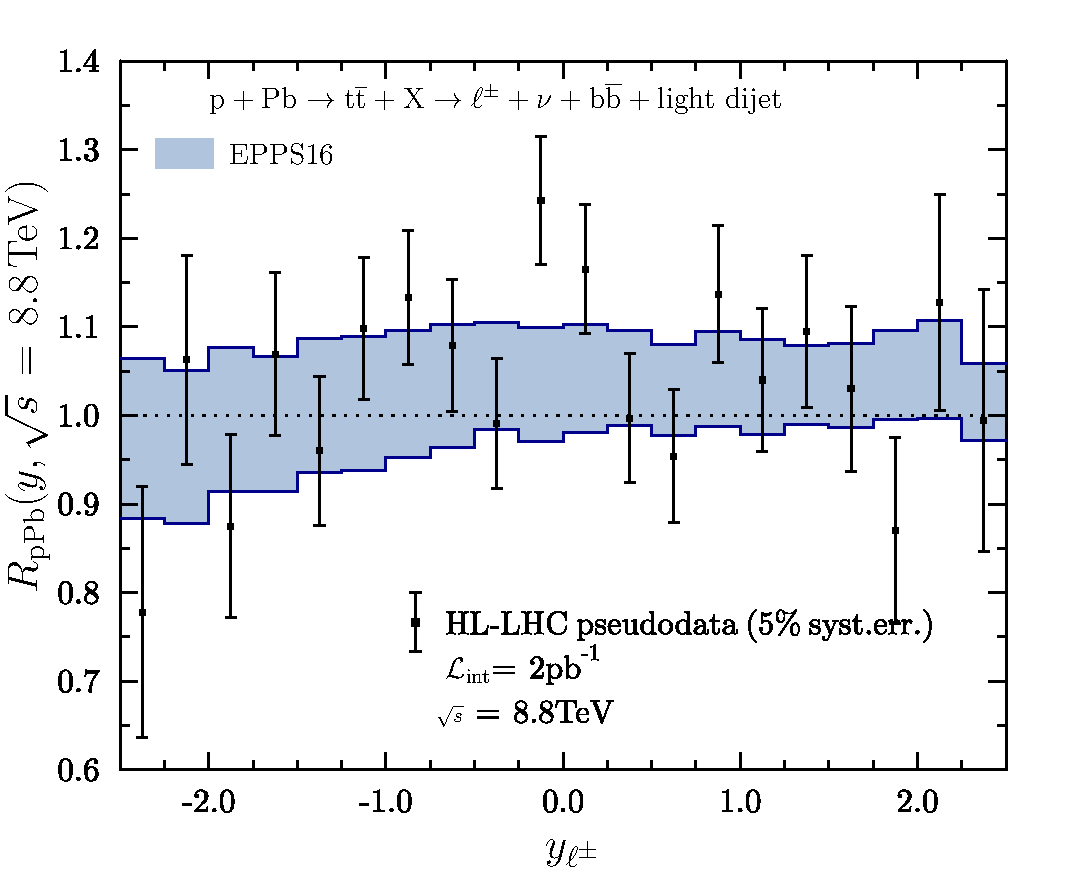
\includegraphics[width=0.495\textwidth]{\main/smallx/fig/ttbardiffy.pdf}
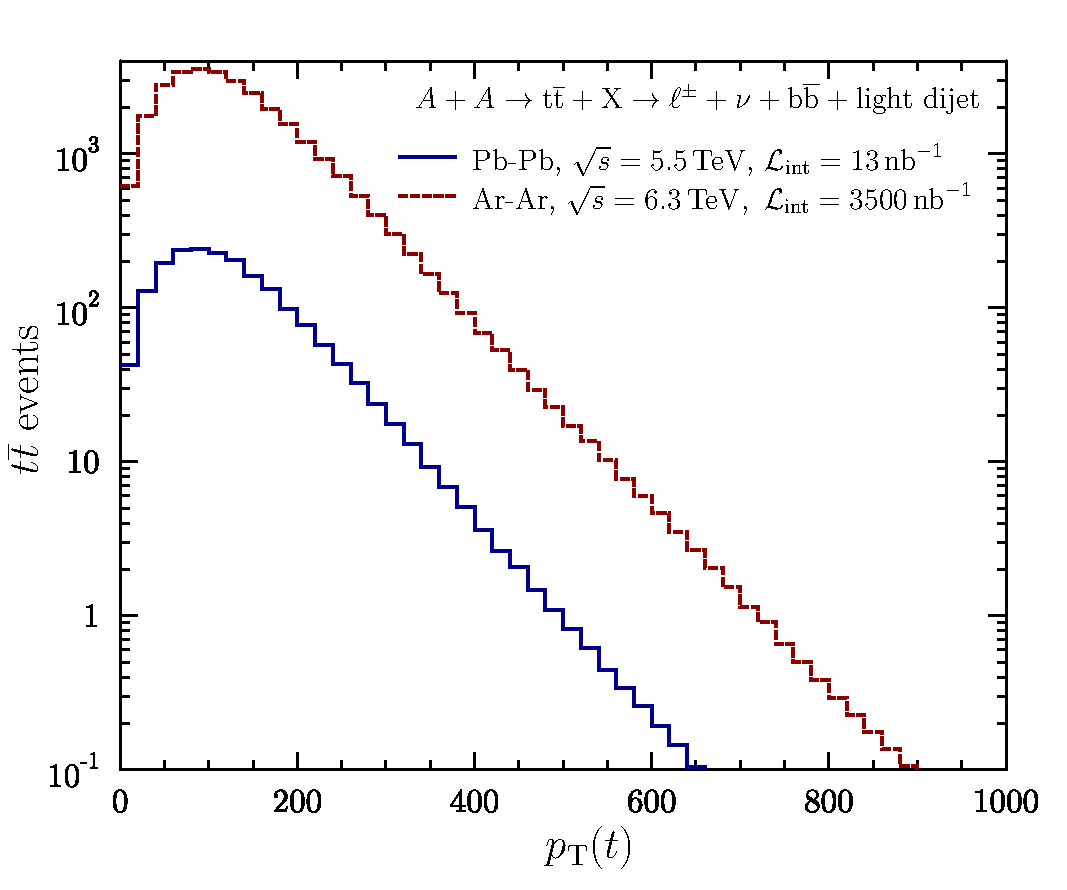
\includegraphics[width=0.495\textwidth]{\main/smallx/fig/pTreach_in_AA.pdf}
\caption{Left: Projected HL-LHC data for $t\overline{t}$ production compared with EPPS16 errorbands. Right: Number of expected $t\overline{t}$ events in $A$-$A$ collisions as a function of the top-quark transverse momentum.}
\label{fig:ttbardiffy}
\end{figure}

The $t\overline{t}$ production provides a complementary observable to the dijets for probing high-$x$ gluons \cite{dEnterria:2015mgr}. For the very short t-quark life time, they decay, in practice exclusively, to W~boson and b~quarks. Although, the cleanest channel is the one where both W bosons decay leptonically, it has been recently demonstrated~\cite{Sirunyan:2017xku} that it is possible to get a clear signal when one of the two W~bosons decays leptonically and the other one goes to light-quark jets. This is the preferred observable as the yields are 3 times higher than when both W bosons decay leptonically. We have estimated the cross sections using the MCFM~code \cite{Campbell:2015qma}, process 146 (where the leptonically decaying W comes from top quark) at NLO level. We have applied the following fiducial cuts:
$$ \pT^{\ell^\pm} > 30 \, {\rm \UGeVc}, \ |y^{\ell^\pm}| < 2.5, \ \pT^{\rm missing} > 30 \, {\rm \UGeVc}, $$
$$ \pT^{\rm jets} > 30 \, {\rm GeV}, \ |y^{\rm jets}| < 2.5, R_{\rm isolation}^{\rm jets} = 0.5. $$

In this setup, the NLO calculation with the factorization and renormalization scales set to the top-quark mass yields, per-nucleon, $\sigma_{\rm n-n} \approx 4200 \, {\rm fb}$ in p-Pb collisions at $\sqrt{s} = 8.8 \, {\rm TeV}$, with CT14NLO~\cite{Dulat:2015mca} proton PDFs and EPPS16~\cite{Eskola:2016oht} nuclear corrections. This is to be multiplied by a factor two to account for the electron and muon final states and by a factor of two to account for the process where the antitop is the one from which the leptonically decaying W originates from. Since this is the nucleon-nucleon cross section, we have to still multiply by a factor of 208 to get the p-Pb cross section. This yields $\sigma_{\rm p-Pb} \approx 3.5 \, {\rm nb}$. Considering the 2000$\, \rm nb^{-1}$ scenario, and efficiency of 0.75~\cite{dEnterria:2015mgr} in b-jet tagging, we expect around 5200 events. Based on this number, we have estimated the expected nuclear modification factor $R_{\rm pPb}$ following the steps of Ref.~\cite{dEnterria:2015mgr}, assigning each data point a 5\%~uncorrelated systematic uncertainty (in the current p-Pb measurement of CMS~\cite{Sirunyan:2017xku} the systematic uncertainty is $\sim$20\%). Dividing the $|y^{\ell^\pm}| < 2.5$ interval to 20 bins, the statistical uncertainty varies from 5\% ($|y^{\ell^\pm}| < 1$) to 10\% (most forward/backward). The resulting $R_{\rm pPb}$ is compared in Fig.~\ref{fig:ttbardiffy} with the EPPS16 uncertainty band. In the considered kinematic configuration the expected $R_{\rm pPb}$ is typically a bit above unity for the gluon antishadowing in EPPS16. As can be seen from the left-hand panel of Fig.~\ref{fig:ttbardiffy}, the expected precision of the measurement is not enough to give significant constraints on nuclear PDFs. In particular, the dijets considered in Section 11.4.3 will probe the same kinematic configuration with a clearly higher precision. However, here much depends on the expected systematic error (taken here to be 5\% for each data point separately) and how large are the bin-to-bin correlations. In the p-Ar mode, the higher c.m. energy of $\sqrt{s} \approx 9.4 \, {\rm TeV}$ increases the yields around 50\% and would also benefit from the higher luminosities, see the next subsection and Sec.~\ref{sec:lightions}.

%This, plus a higher achievable nucleon-nucleon luminosity ($\sqrt{10} \approx 3$, based on John Jowett email on 7.9.2018 + his slides) would render the above case almost completely systematics dominated. \ref{sec:lightions}

%Using the same framework and assumptions as above, we have estimated the fiducial $t\overline{t}$ yields is $A$-$A$ collisions. Here, we have considered Pb-Pb and Ar-Ar cases. In Pb-Pb configuration with $\sqrt{s_{\rm NN}} = 5.5 \, {\rm TeV}$, the per-nucleon cross section is $\sigma_{\rm n-n} \approx 1200 \, {\rm fb}$ which translates to around 2000 reconstructed events for 13$\, \rm nb^{-1}$ ion-ion luminosity. In the Ar-Ar option, the c.m. energy is slightly higher, $\sqrt{s} = 6.3 \, {\rm TeV}$, which increases the cross-section by some 50\%. In addition, the achievable ion-ion luminosity is much higher, 3500$\,\rm nb^{-1}$ (semi-optimistic estimate from John Jowett's slides). Thus, the estimated amount of $t\overline{t}$ events is clearly larger, around 30000. The right-hand panel of Fig.~\ref{fig:ttbardiffy} shows the event distributions as a function of top-quark transverse momentum $\pT(t)$. This shows that, the HL-LHC may allow to probe the space-time picture of heavy-ion collisions using top quarks \cite{Apolinario:2017sob} up to $p_{\rm T}(t) \approx 400\,{\rm GeV}$ in the Pb-Pb case, and up to $p_{\rm T}(t) \approx 700\,{\rm GeV}$ in the Ar-Ar alternative. \\



%the power to constrain large x gluons vs the heavy quark which is lower x

%Czakon et al., Pinning down the large-x gluon with NNLO top-quark pair
 %                       differential distributions   \cite{Czakon:2016olj}


\subsection{Perspectives with lighter ions}
%To be confirmed, lumis to be given in the accelerator part \\
%Editors: Nestor Armesto, Fred Olness \\
%Indicative length: 1-2 pages \\

Lighter ions, with the possibility to achieve large integrated luminosities in modest running times, see Sect.~\ref{sec:lightions} in the accelerator chapter, offer several interesting opportunities for the study of the initial stage of ion collisions, for small-$x$ physics and for the determination of nuclear parton densities, see Subsection \ref{sec:smallxIntro}.

First, concerning nPDFs, it should be noted that due to the scarcity of nuclear data, a PDF fit for a single nucleus is impossible as discussed in Subsection \ref{sec:smallxIntro}. The different groups \cite{deFlorian:2011fp,Kovarik:2015cma,Eskola:2016oht}  have adopted different strategies but, generically, they give the parameters in the initial condition to be fitted a dependence on the nuclear mass number. Such dependence acquires different functional forms and, therefore, it constitutes part of the parametrisation bias in the nPDF set. Data on lighter nuclei may help to constrain such parametrisations, see the discussions for UPCs and pA collisions in Subsection \ref{sec:nPDFs}.

On the other hand, the impact parameter dependence of nPDFs is linked to their dependence on nuclear size. Several models exist (see e.g. \cite{Emelyanov:1998phs,Ferreiro:2008wc}), and even less model-dependent approaches like the EPS09s analysis \cite{Helenius:2012wd} where the dependence on nuclear size was used to constrain the impact parameter dependence. Besides, first-principle calculations combining Gribov theory of inelastic shadowing and factorization theorems for hard diffraction and DIS relate diffraction in electron-proton collisions with nuclear shadowing. This has been used to predict nuclear shadowing \cite{Frankfurt:2011cs,Armesto:2003fi}, including its nuclear size and impact parameter dependence. While such relation is exact for deuteron, its extension to larger nuclei has some degree of model-dependency. Lighter ions are the ideal place to test the nuclear size dependence without resourcing to centrality selection, whose relation with impact parameter is doomed to be as problematic - at least - as found in pPb collisions at the LHC.

Lighter ions also offer large luminosities that are important for several aspects:
\begin{itemize}
\item Data on beauty mesons and bottomonium in pA can be used to constrain nPDFs \cite{Kusina:2017gkz} better than their charm counterparts, because of the larger scale given by the mass and by the opportunity that they are less affected by collective effects. But they demand large statistics that can be achieved with lighter ions.
\item Larger luminosities will benefit measurements in pA for observables with large scales, like high-mass DY or dijets, for precise determination of nPDFs.
\item UPCs and photon-photon studies \cite{Baltz:2007kq} will be greatly benefited in spite of the $Z^{2(4)}$ factor for the photon luminosities that can be overcompensated by the larger nucleon-nucleon luminosity .
\item Larger luminosities can also benefit small-$x$ forward observables that, like dijets \cite{Dainese:2016gch}, aim to reach quite large transverse momenta.
\end{itemize}

Lighter ions offer a bridge between small systems and PbPb without requiring centrality selection that is problematic both in pp, pA and peripheral AA. 
Besides, in the framework of saturation models \cite{Gelis:2010nm} that aim to describe collective effects in small systems without requiring final state interactions (see e.g. \cite{Kovner:2016wsq} and references therein), the extension from the proton to the nuclear case in phenomenological realizations  is done by a simple rescaling of the squared saturation momentum $Q_s^2\propto A^{1/3}$. And the centrality dependence is assumed to be proportional to the nuclear profile, which leads to strong problems in the nuclear periphery where a dilute situation is restored. Lighter ions offer a check of our ideas on the
nuclear size versus energy leading
the density that determines saturation, and the use of minimum bias observables
instead of centrality-sliced ones that
would greatly simplify the phenomenology.

To conclude, lighter ions offer several pros and cons for initial stage studies. The main con is the fact that theory calculations usually assume the limit of scattering of a dilute projectile (proton) on a dense target (nucleus). Lighter ion-ion collisions are further from this limit. On the other hand, they offer: (i) a bridge between small and large systems without resourcing to
centrality selection that would be useful for constraining the nuclear wave function, the
collision dynamics and the interpretation of collectivity;
(ii) the possibility of larger luminosities for UPCs, forward observables,$\dots$,
for nPDFs determination and small-x studies; and (iii)
a more affordable setup for microscopic calculations of corrections.

\end{document}
  

\end{document}
